\documentclass[letter,12pt]{book}
\usepackage[spanish]{babel}
\usepackage[bookmarks]{hyperref}

\usepackage[utf8]{inputenc}
\usepackage{lmodern}
\usepackage{graphicx}
\usepackage{epstopdf}
\usepackage{pdflscape}
\usepackage{array}
\usepackage{hvfloat}
\usepackage{apacite} 
\usepackage{chngcntr} %para numeracion de figuras
\usepackage{mathtools}
\usepackage{supertabular}
\usepackage{longtable}
\usepackage[table,xcdraw]{xcolor}
\graphicspath{ {./imagenes/} }
\setcounter{secnumdepth}{3} % para que ponga 1.1.1.1 en subsubsecciones...
\setcounter{tocdepth}{3} % para que añada las subsubsecciones en el indice...


\let\tmp\oddsidemargin
\let\oddsidemargin\evensidemargin
\let\evensidemargin\tmp
\reversemarginpar

\makeatletter
\renewenvironment{thebibliography}[1]
     {\chapter*{\bibname}% <-- this line was changed from \chapter* to \section*
      \@mkboth{\MakeUppercase\bibname}{\MakeUppercase\bibname}%
      \list{\@biblabel{\@arabic\c@enumiv}}%
           {\settowidth\labelwidth{\@biblabel{#1}}%
            \leftmargin\labelwidth
            \advance\leftmargin\labelsep
            \@openbib@code
            \usecounter{enumiv}%
            \let\p@enumiv\@empty
            \renewcommand\theenumiv{\@arabic\c@enumiv}}%
      \sloppy
      \clubpenalty4000
      \@clubpenalty \clubpenalty
      \widowpenalty4000%
      \sfcode`\.\@m}
     {\def\@noitemerr
       {\@latex@warning{Empty `thebibliography' environment}}%
      \endlist}
\makeatother

\setlength{\parskip}{1ex}

\newcolumntype{L}[1]{>{\raggedright\let\newline\\\arraybackslash\hspace{0pt}}m{#1}}
\newcolumntype{C}[1]{>{\centering\let\newline\\\arraybackslash\hspace{0pt}}m{#1}}
\newcolumntype{R}[1]{>{\raggedleft\let\newline\\\arraybackslash\hspace{0pt}}m{#1}}

\begin{document}

  \begin{titlepage}

    \begin{center}
      \vspace*{-1in}
      \begin{figure}[htb]
    \begin{center}
      \includegraphics[width=8cm]{imagenes/Logo_Distrital.eps}
    \end{center}
    \end{figure}

    FACULTAD DE INGENIERÍA\\
    \vspace*{0.15in}
    PROYECTO CURRICULAR DE INGENIERÍA DE SISTEMAS \\
    \vspace*{0.6in}
    \begin{large}
    Proyecto:\\
    \end{large}
    \vspace*{0.2in}
    \begin{Large}
    \textbf{VERSION COMPLETA: DISEÑO E IMPLEMENTACIÓN DE UN PROTOTIPO DE SNS ORIENTADO AL DEPORTE SOBRE TECNOLOGÍAS MÓVILES} \\ 
    \end{Large}
    \vspace*{0.3in}
    \begin{large}
    Presentado por:\\
      Nicolás Mauricio Garcia Garzon 20091020031 \\
      Luis Felipe Gonzalez Moreno 20091020035
    \end{large}
    \vspace*{0.3in}
    \rule{80mm}{0.1mm}\\
    \vspace*{0.1in}
    \begin{large}
    Dirigida por: \\
    Doctor Carlos Enrique Montenegro Marin \\
    Coodirector: \\
    Paolo Alejandro Daza Corredor \\
    \end{large}
    \end{center}

    \end{titlepage}



  \newpage
  \mbox{}
  \thispagestyle{empty} % para que no se numere esta página
  
  \tableofcontents % indice de contenidos

  \cleardoublepage
  \addcontentsline{toc}{chapter}{Lista de figuras} % para que aparezca en el indice de contenidos
  \listoffigures % indice de figuras

  \cleardoublepage
  \addcontentsline{toc}{chapter}{Lista de tablas} % para que aparezca en el indice de contenidos
  \listoftables % indice de tablas
  
  \counterwithout{figure}{chapter}
  \counterwithout{table}{chapter}
  
  \chapter*{Introducción} % si no queremos que añada la palabra "Capitulo"
  \addcontentsline{toc}{section}{Introducción} % si queremos que aparezca en el índice
  \markboth{INTRODUCCIÓN}{INTRODUCCIÓN} % encabezado
  El uso de los medios informáticos para la formación de comunidades deportivas en las que los deportistas puedan formar y gestionar sus redes sociales es restringido debido al modo de vida del deportista. Es usual que por medio de facebook y twitter los deportistas creen sus redes sociales. Sin embargo, facebook y twitter añaden información basura para los deportistas y no ofrecen servicios que han de ser propios de una red social deportiva.

En este documento se expone una propuesta para el desarrollo de una red social deportiva por medio de la teoría de redes sociales, SOA, BPMN y la investigación del estado del arte de las redes sociales deportivas. Lo que se pretende con el documento es exponer el problema existente que hay entre la utilización de las TIC y la comunicación (a modo de red social) entre las comunidades deportivas. Además, también se pretende, en el presente documento, dar una solución basándose en el análisis de la información existente en cuanto al problema formulado y el armado de un proceso de ingeniería para llevarla a cabo.

Primero, el lector encontrará un acercamiento al problema que se resolverá en la definición del problema, la justificación y los objetivos. Más adelante, el lector podrá echar un vistazo a la teoría que está detrás del problema a resolver y que es necesaria para su solución. Por último, se presenta al lector el marco a utilizar para la solución del problema en las secciones de metodología, cronograma y un estudio de presupuestos.

  
  \chapter*{Glosario}
  \addcontentsline{toc}{section}{Glosario} % si queremos que aparezca en el índice
  \markboth{GLOSARIO}{GLOSARIO} % encabezado
  \begin{itemize}
  \item OSN : Online Social Network – Red Social En-línea, es una red social que crece dentro del ámbito web.
  \item SNS : Social Network Services – Servicios de Redes Sociales.
  \item Offline Social Network : Red social que crece en el ámbito real, no en el virtual como lo es en las OSN.
  \item Sistemas transversales : Sistemas que interactúan entre sí, hechos o no con tecnologías diferentes sobre paradigmas diferentes, con un fin común.
  \item API : Application Programming Interface – Interfaz de programas de aplicación, es el conjunto de funciones y procedimientos de un sistema que pueden ser utilizados en otro sistema. Es el puente de conexión entre ambos sistemas.
  \item Interoperabilidad : Capacidad de un sistema de software para trabajar con otro sistema con la característica de que esta cooperación sea hecha de la manera más transparente posible.
  \item SOA : Service-Oriented Architecture – Arquitectura Orientada a Servicios.
  \item TI : Tecnologías de la Información
  \item ROI : Return on investment – Retorno en inversión.
  \item Product Backlog : Productos que están pendientes por realizar para finalizar el proyecto.
  \item Sprint Goal : El objetivo, que de cumplirse, determina si el Sprint fue exitoso.
  \item Nodo : Punto de intersección de varios elementos
  \item Arista : Uniones entre nodos
  \item StakeHolders : Partes interesadas en un tema específico.
  \item UX (User eXperiencie): Se refiere a la percepción que adquiere el usuario de un dispositivo (software, hardware) con respecto a las tareas realizadas con este, basándose en las sensaciones/reacciones que este le provoca.
\end{itemize}

  
  \chapter{Definición del problema}
  \label{chap:definicion_problema}
  El hombre, en su continua evolución, ha utilizado el lenguaje como una herramienta creadora de conocimiento transferible a sus congéneres o cualquier otro ser que interactuase con él. Con esto, “los humanos han desarrollado el lenguaje como un instrumento ligero y conveniente para mantener sus relaciones”\cite{dynamics}. 

En la comunicación entre congéneres, el lenguaje puede ser dividido en dos funciones: función de transmisión de información (gossip) y función de entendimiento del estado interno (estado mental) del congénere (mentalisation)\cite{dynamics}. Estas funciones de transmisión y entendimiento del otro han permitido que dos o varios humanos puedan asociarse entre sí formando redes sociales.

Las redes sociales no son otra cosa que la formación de lazos de algún tipo (emocional, de pertenencia a una comunidad, de trabajo, etc.) entre individuos que pueden ser organizaciones o humanos.\cite{sna_startups} En la figura \ref{fig:red_al_quaeda} puede verse cómo es representada la red social que forman las células terroristas de Al-Qaeda.

\begin{figure}[!htb]
  \begin{center}
    \includegraphics[width=11cm]{./imagenes/red_al_qaeda.png}
    \caption{Red social conformada por las células terroristas de Al-Qaeda.}
    \label{fig:red_al_quaeda}
  \end{center}
\end{figure}

La evolución de los servicios proporcionados a través de la internet ha sido drástica puesto que ha cambiado el modo de vida de las personas. En la figura \ref{fig:utilizacion_internet} se evidencia el crecimiento de la internet (de los servicios que en ella se soportan) se da en función de los servicios de conectividad social que son creados y soportados en ella. La web 1.0 fue utilizada en mayor medida por científicos para el intercambio de información en formato hipertexto. No había una interacción fuerte entre cada científico sino que ellos acudían a internet para buscar o poner a disposición material científico. Con la venida de la web 2.0 y la introducción de la interacción del usuario con la web generando contenido en tiempo real, así se crearon servicios de redes sociales en-línea (OSN en inglés: On-line Social Network), produciento una partición en los tipos de redes sociales. Así, las redes sociales a las que pertenece el ser humano en la era digital se dividieron convenientemente en “redes sociales fuera de línea” y redes sociales en línea (Offline Social Network y Online Social Network).

\begin{figure}[!htb]
  \begin{center}
    \includegraphics[width=11cm]{./imagenes/utilizacion_internet.png}
    \caption{Cambio de la utilización de internet en función de los servicios de conectividad social que son creados y soportados en ella}
    \label{fig:utilizacion_internet}
  \end{center}
\end{figure}

Las redes sociales fuera de línea son las redes sociales que se forman por comunicación tradicional (lenguaje oral y escrito en medios que difieran de aquellos que utilizan las telecomunicaciones). Las redes sociales en línea son aquellas redes sociales que están formadas por cibernautas y en las cuales la comunicación se da por medio de los servicios de redes sociales.

La administración de una red social fuera de línea fue estudiada desde inicios del siglo XX\cite{dynamics} con un enfoque socio-matemático llamado “análisis de redes sociales” (SNA por sus siglas en ingles: Social Network Analisis). Sin embargo, era difícil el análisis del comportamiento humano según los designios de la SNA puesto que la información debía ser recopilada por medio de entrevistas a las personas. Aún así, el enfoque SNA fue utilizado para analizar el comportamiento terrorista o inclusive el comportamiento de trabajadores en una empresa.\cite{sna_startups}

Con la creación de las OSN y la gran cantidad de información que describe el comportamiento humano sobre este tipo de red social, ha sido más sencillo utilizar el enfoque de la SNA para estudiar que comportamientos tienen los humanos sobre una red social establecida.

Los servicios de redes sociales (SNS por sus siglas en ingles: Social Network Services) como Facebook, LinkedIn, Twitter, SportTracker o Xportia, ofrecen servicios para la gestión de la OSN de cada usuario que acceda a estas aplicaciones. Según un estudio hecho para medir la experiencia de usuario (UX por sus siglas en ingles: User eXperience) en los SNS, se encontraron 8 categorías que son críticas a la hora de diseñar una SNS y son:

1. Self-expresion: Capacidad que tengan las OSN de compartir contenido relacionado a la vida real de los usuarios tal como lo pueden ser las fotos, los videos, los comentarios o las comunicaciones directas.
2. Reciprocity: Interacción bilateral en tiempo real, es decir, interacción instantánea con uno o varios individuales en la OSN (por ejemplo, por medio de los servicios de mensajería instantánea).
3. Learning: La información recibida por medio de la OSN debe poder ser utilizada en pro del desarrollo cognitivo del individual; debe existir información útil al individual que usa la OSN.
4. Curiosity: El contenido de la OSN debe ser interesante para quien la utiliza.
5. Suitability of functionality: Se refiere a cuán “utilizable” es una funcionalidad.
6. Suitability of content: La calidad y exactitud de la información que en la OSN reside debe ser suficiente para el individual perteneciente a ella.
7. Completeness of the user network: Los individuales deben querer pertenecer a la red social y buscar eficientemente a otros individuales para poder formar lazos con ellos y hacer crecer su red social.
8. Trust and privacy: Confianza en los servicios de las OSN, así como también la capacidad que tiene el usuario de gestionar la privacidad del contenido que comparte en dicha OSN.\cite{social_experience}

De acuerdo al enfoque SNA, las redes sociales pueden estar divididas en clusters, que no son más que agrupaciones de individuales sobre una red social por algún concepto como, por ejemplo, la pertenencia a una comunidad. Con lo anterior, podemos encontrar que algunos SNS ofrecen servicios para gestionar las OSN de sus usuarios centrándose en algún tipo de comunidad en específico y, la información que circula por ese tipo de comunidades, es diferente a la que pasa por SNS descentralizados (como Facebook y twitter). Viendo Facebook como una agrupación de clusters con temáticas tan diferentes como lo son los deportes y la música, la ciencia y la vida cotidiana, se puede decir que algunos SNS se enfocan en alguna de estas temáticas. En este caso, el cluster o temática que compete al trabajo a elaborar es el deporte.

Es posible hacer una división del cluster deporte en otros subclusters de cada uno de los deportes que existen en el mundo o en la clasificación de los deportes que han dado organizaciones como, por ejemplo, la IWGA (Internation WorldGames Association). Lo que se quiere con este trabajo es aportar al crecimiento de las redes sociales fuera de linea de las personas que practiquen deporte sin importar si lo hacen a nivel profesional o aficionado por medio de un SNS orientado a los deportes en general y, por lo tanto, el cluster que se ha escogido para trabajar es el del deporte como cluster mismo.

Se investigó acerca de las redes sociales existentes enfocadas a la temática del deporte y se encontró que muchas de ellas son utilizadas en mayor medida en España y que todas ellas están soportadas sobre tecnologías web. En general, solo se encontraron dos redes sociales deportivas orientadas a cualquier deporte asociadas a aplicaciones para smartphones disponibles en el la tienda virtual de Android o en la tienda virtual de Apple (La red social de Fitivity y Huddlers).

Así, con la evolución de la comunicación humana trasladándose a los espacios virtuales por medio de las OSN y la falta de aplicaciones, en el campo de los smartphones, que soporten interacciones sociales enfocadas a los deportes en general, en este trabajo se creará un SNS centrado en los deportes sobre tecnologías Android para la administración de las OSN de cada persona en un ámbito deportivo desde su dispositivo móvil.

  
  \chapter{Justificación del problema}
  \label{chap:justificacion}
  Los humanos, desde siempre en su evolución, han necesitado de mecanismos para comunicarse con sus congéneres. En la actualidad, uno de los mecanismos es el uso de los SNS como facebook y twitter, cada uno de ellos modificando la forma de creación de redes sociales en la actualidad. (Sección \ref{sec:red})

De acuerdo al análisis egocéntrico de las redes sociales de cada individuo, se hace conveniente la utilización de SNS para gestionar las relaciones que un individuo mantiene con otros individuos (sean personas u organizaciones) en los diferentes círculos sociales en los que se mueve. (Sección \ref{sec:egocentrico})

El círculo social o comunidad escogida para el desarrollo propuesto es la comunidad deportiva debido a que hay mucha información dispersa alrededor de internet que es ambigua y a veces inclusive errónea. A su vez, debido a que gran cantidad de deportes no han tenido una acogida grande alrededor del mundo, las comunidades que se mueven sobre uno de esos deportes son más cerradas y, por ende, pequeñas y con poca información para un público que salga de las fronteras de dichas comunidades cerradas. Lo que se quiere con este trabajo es aportar al crecimiento de las redes sociales de las personas que practiquen deporte sin importar si lo hacen a nivel profesional o aficionado por medio de un SNS orientado a los deportes en general.

Un factor de utilización masiva de las SNS es que éstas estén orientadas a un público en particular y aumenten su cobertura dependiendo de su alcance de masa crítica sobre una red social definida \cite{sna_startups}. Al construir, en principio, la red social deportiva enfocada en dos deportes en particular, la probabilidad de ganar la masa crítica es mayor y, por tanto, el SNS desarrollado puede volverse más útil con el tiempo.

La UX de los SNS (visto en la sección \ref{sec:UX}) es otro factor, debido a que juega un papel importante pues es esta la segunda carta de presentación de un SNS. Algunas de las características que evalúan los usuarios en cuanto a la UX no son suplidas por los SNS actuales – o al menos no parcialmente - , tres de ellas (fundamentales para la acogida de un nuevo SNS) son “curiosity, learning y completeness of the social network”. Así, habiendo analizado 19 SNS orientados al deporte (Tablas \ref{tab:comparacion_redes_1} a \ref{tab:comparacion_redes_5}), se concluyó que fallaban en alguna de las tres características mencionadas.

Tener en cuenta la población a quien va dirigido el SNS a desarrollar es otro factor de éxito. Según \cite{user_behavior_online}, entre los años de adolescencia y los 40 años de edad, las personas acuden con mayor interés al uso de los SNS; al ser la comunidad del deporte comprendida en su mayoría por personas entre la adolescencia y los 40 años, aumenta aún más la probabilidad de alcanzar la masa crítica y volver útil con el tiempo el SNS.

Un último factor, que se observó, afecta la creación de redes sociales (tanto fuera de línea como en línea) (Sección \ref{sec:red}) es la distancia entre cada individual y el posible tipo de enlace que los uniría. Al ver la importancia de manejar SNS que ofrezcan servicios de geolocalización, se ha visto pertinente añadir dicho servicio a la creación del prototipo de SNS orientado a los deportes en general.

También se encontró evidencia de poca utilización de los SNS que no estaban orientadas a móviles. Dichos SNS eran utilizados mucho más por personas
que practican deportes que empiezan a tomar vuelo o deportes poco conocidos (un ejemplo de ello es el padel). El problema con dichos SNS es la
naturaleza nómada de los deportistas. Una solución a la naturaleza nómada de los deportistas y el acercamiento de los últimos a las TICs y, en este caso, a
los SNS deportivos es la aparición y utilización en masa de los smartphones.

En general, solo se encontraron dos redes sociales deportivas orientadas a cualquier deporte asociadas a aplicaciones para smartphones disponibles en el la tienda virtual de Android o en la tienda virtual de Apple (La red social de Fitivity y Huddlers) (Tablas \ref{tab:comparacion_redes_1} a \ref{tab:comparacion_redes_5}). Además, hay una ventaja real en hacer una red social orientada a dispositivos móviles y es la capacidad de movilidad que ellos brindan mientras se está utilizando el servicio \cite{spiderweb}. Dada la falta de aplicaciones móviles en el campo descrito y a su vez la importancia que toman los dispositivos móviles por sus características, se ha decidido hacer el prototipo de SNS orientado al deporte sobre tecnologías móviles.

  
  \chapter{Objetivos}
  \label{chap:objetivos}
  \section{Objetivo General}
   Desarrollar un prototipo SNS (Social Networking Service) centrado en el deporte, sobre tecnologías Android, que permita al usuario el acceso a diferentes servicios propios de una red social con el fin de fortalecer a las comunidades que practican deporte, y a quienes quieren ser parte de ellas, facilitando la comunicación y el acceso a la información a los usuarios de la red.

  \section{Objetivos específicos}
   \begin{itemize}
  \item Investigar acerca de la teoría de las redes sociales, la computación orientada a servicios y el estado del arte de las redes sociales, con el fin de que el prototipo a desarrollar esté cimentado sobre bases teóricas sólidas.
  \item Identificar, analizar y evaluar las necesidades de la comunidad deportiva concernientes al SNS a implementar y, posteriormente, postular requerimientos funcionales y no funcionales para el SNS.
  \item Formular una arquitectura híbrida bajo el paradigma SOA que cumpla los diferentes requerimientos del proyecto, con el fin de tener un marco de trabajo que soporte cada etapa posterior a la formulación de esta.
  \item Postular, escoger y diseñar los servicios que darán solución a los requerimientos y necesidades identificadas para la implementación de la SNS, con el fin de gestionar cada incremento del proyecto y escoger los servicios a diseñar.
  \item Implementar y probar los diferentes servicios con el fin de cumplir los requerimientos planteados en la fase de análisis.
\end{itemize}


  \chapter{Alcances y limitaciones}
  \label{chap:alcances_limitaciones}
  A continuación el lector podrá encontrar los alcances y las limitaciones del presente proyecto.

\section{Alcances}

A continuación se presenta un breve recuento de las funcionalidades y aspectos tecnológicos que se tienen en cuenta en el desarrollo del prototipo, así cómo también se especifican los deportes que son soportados por el prototipo. Además, se da una alineación de lo expresado anteriormente con la solución que da el prototipo a los problemas encontrados en la sección \ref{cap:estado_arte} y justificados en el capítulo \ref{chap:justificacion}

\subsection{Aspectos tecnológicos}

Este proyecto pretende diseñar e implementar un prototipo de SNS orientado al deporte bajo dispositivos móviles ANDROID, utilizando una arquitectura orientada a servicios que facilite el desarrollo y la interoperabilidad con diferentes sistemas que existan actualmente en el mercado. Para esto, se utilizará el entorno de desarrollo que brinda Android a los desarrolladores en conjunto con los diferentes dispositivos disponibles para el desarrollo del proyecto.

Las funcionalidades que se ha decidido implementar para el prototipo son:

\begin{enumerate}

	\item Soporte de información de usuario, donde el usuario pueda tener su propio perfil con información personal 
	
	\item Soporte de información deportiva de los deportes que son implementados por la red social deportiva

	\item Debido a la escogencia de tecnologías móviles para el desarrollo del trabajo, se ha decidido incluir funcionalidades de geolocalización y demás de las que dependa ésta. Las funcionalidades que utilizan el componente de geolocalización son:

\begin{itemize}
  \item Ubicación de lugares deportivos por parte de usuarios del SNS
  \item Cercanía a eventos deportivos por parte de un usuario del SNS
  \item Cercanía entre usuarios del SNS que compartan una relación (sea simétrica o asimétrica). Para el caso del prototipo, se manejan dos características públicas: el o los deportes jugados por el usuario y si se encuentra jugando un determinado deporte. De manera que la relación que compartirán los usuarios será de deporte practicado.
\end{itemize}

\end{enumerate}

\subsection{Aspectos de negocio}

En cuanto a los deportes, se ha decidido realizar (en la etapa de análisis), encuestas a la población universitaria (como se puede ver en el capítulo \ref{chap:modelo_datos}) para averiguar, además de si era o no valiosa la creación del SNS, que deportes pueden ser los candidatos a implementar sobre el SNS a desarrollar, teniendo como pauta la siguiente aseveración: Los deportes, resultado de la encuesta, elegidos, serán aquellos que en su participación sean los de menor población practicante. Al final, se ha decidido que el SNS se enfocará en los deportes Rugby y Tenis para la etapa de construcción del prototipo.

\subsection{Alineación de aspectos tecnológicos y de negocio con la solución del problema}

El prototipo de SNS deportivo desarrollado con los alcances dados en los aspectos de negocio y tecnológicos se acopla a la finalidad que se le ha dado: Por un lado, la capacidad de éste de ser herramienta de un deportista para la gestión de su red social deportiva, brindando al deportista la capacidad de conocer la ubicación de juego de los deportes seleccionados, así como también de estar al tanto de los eventos sobre un deporte específico. Debido a la capacidad primera del prototipo de brindar ubicaciones de usuarios que compartan una relación deportiva, el usuario será capáz de saber si en un lugar podrá encontrar una cantidad, para él, aceptable de personas para poder practicar su deporte y ampliar su red social offline; por otro lado, el SNS deportivo se ajusta a la característica nómada de los deportistas dado que será desarrollado sobre plataformas móviles.

\section{Limitaciones}

Entre las diferentes limitaciones que se pueden encontrar en el desarrollo del actual proyecto, se encuentran las siguientes:

\begin{itemize}
  \item \textbf{Disponibilidad de dispositivos de prueba:} Ya que en el mercado existe una gran cantidad de dispositivos móviles, todos con diferentes especificaciones, es imposible garantizar que la aplicación a diseñar sea soportada por todos los dispositivos del mercado. Sin embargo, se tienen diferentes dispositivos, entre tablets y celulares, en donde se pueden realizar las pruebas (referenciados en los recursos de hardware, capítulo \ref{chap:costos}), limitando los dispositivos soportados oficialmente por el prototipo.

  \item \textbf{Disponibilidad de equipos a usar como servidores:} Ya que el proyecto se basa en la creación de un prototipo, se utilizarán los computadores personales disponibles para proveer los servidores que se necesiten, limitando el rendimiento que de los mismos.
  
  \item \textbf{Recolección de información}: La búsqueda de información se hará sobre la ciudad de Bogotá, haciendo énfasis en la comunidad universitaria, lo cuál sesgará la información a aquella válida sobre una comunidad con edades que oscilan entre los 15 y los 25 años y, a su vez, sobre las preferencias en universidades respecto a tendecias deportivas y no sobre la población bogotana entera.
  
  \item \textbf{Utilización de software libre y con fines académicos:} Será utilizado, en su mayoría, software libre para la realización del proyecto, así como también software que preste licencia con fines académicos, debido a que no se cuenta con el presupuesto necesario para probar herramientas privativas (a parte de versiones de prueba) que pudieran llegar a ser mejores que sus homólogos libres.
  
  \item \textbf{Etapas del ciclo de vida del software no contempladas:} No se llevará acabo una etapa de implantación del software debido a que éste prototipo, aunque funcional, no estará direccionado de inmediato al mercado próximo ya que, debido a las limitaciones de tiempo de los autores, no será posible implementar todos los requerimientos no funcionales que se llegaran a dar al SNS. Por supuesto, al no haber una etapa de implantación, para este trabajo tampoco será presentada la etapa de mantenimiento.
\end{itemize}

  
  \chapter{Trabajos futuros}
  Debido al corto tiempo que se ha propuesto para la realización del proyecto y los costes que puede generar el hacer más funcionalidades, en siguientes iteraciones de éste proyecto se harán las siguientes funcionalidades:

\begin{itemize}
	\item Reportes estadísticos de la cantidad de personas que están practicando un deporte en un lugar específico
	\item Un módulo de self-sharing donde los participantes de la red social puedan publicar contenidos en un espacio personal e interactuar con otros en la red por medio de funciones de mensajería instantánea
	\item Manejos de contenidos de salud y de consejos deportivos que se puedan compartir sobre la red social para enriquecer el conocimiento de los participantes de la red
\end{itemize}

  \chapter{Marco conceptual}
  \section{Comunicación}

Los científicos han estudiado el porqué de las relaciones complejas entre los humanos en comparación a la complejidad presentada en las relaciones entre otros animales. Una de las hipótesis, Social Brain Hypothesis (SBH) postula que el crecimiento cognitivo humano y sus intrincadas relaciones sociales se deben a “la necesidad de nuestros ancestros de mantener e incrementar el número de relaciones sociales con diferentes grupos para sobrevivir en las extremadamente desafiantes condiciones ambientales originadas durante la última era glacial”.\cite{dynamics}

El hombre, en su continua evolución, ha utilizado el lenguaje como una herramienta creadora de conocimiento transferible a sus congéneres o cualquier otro ser que interactuase con él. Con esto, “los humanos han desarrollado el lenguaje como un instrumento ligero y conveniente para mantener sus relaciones” \cite{dynamics}. 

En la comunicación entre congéneres, el lenguaje puede ser dividido en dos funciones: función de transmisión de información (gossip) y función de entendimiento del estado interno (estado mental) del congénere (mentalisation) \cite{dynamics}. Estas funciones de transmisión y entendimiento del otro han permitido que dos o varios humanos puedan asociarse entre sí formando redes sociales.


\input{./Capitulos/Marco_teorico/Evolucion_web.tex}

 
  \chapter{Marco teórico}
  \section{Redes Sociales}

\subsection{¿Qué es una red?}

Una red es un conjunto de relaciones. Mas específicamente, una red consiste en un conjunto de objetos (nodos) que están interconectados a través de relaciones (aristas). La red mas simple consiste en 2 nodos, N1 y N2, que están relacionados entre sí (Figura \ref{fig:simple}). Los nodos podrían representar personas, mientras la arista representa la relación que existe entre ellas (N1 y N2 son amigos, por ejemplo).

\begin{figure}[!htb]
  \begin{center}
    \includegraphics{./imagenes/Red_simple.eps}
    \caption{La red mas simple}
    \label{fig:simple}
  \end{center}
\end{figure}

Las relaciones pueden ser simétricas o asimétricas. Cuando se tiene una relación simétrica se dice que la relación no tiene dirección, es decir, la relación puede leerse en ambos sentidos. En el ejemplo anterior, significaría que N1 es amigo de N2 y que N2 es amigo de N1. Para que una relación se considere asimétrica, la relación debe poder leerse en un único sentido, es decir, la relación tiene una dirección determinada. En la figura \ref{fig:asimetrica} se puede observar un ejemplo de una red asimétrica en donde el nodo (o persona) N1 sigue al nodo N2, pero el nodo N2 no sigue al nodo N1.

\begin{figure}[!htb]
  \begin{center}
    \includegraphics{./imagenes/Red_asimetrica.eps}
    \caption{Ejemplo de una red asimetrica}
    \label{fig:asimetrica}
  \end{center}
\end{figure}

Es posible que exista mas de una relación entre 2 nodos, en ese caso se dice que existe una \textit{relación multiplex}

\subsection{Grado de centralidad}

En todas las redes, sean virtuales o no, existen personas que son mas ``importantes" que otras, más \textbf{populares}. Estas celebridades representan una parte muy pequeña de la red, pero debido a su gran influencia siempre es bueno identificarlos. Para esto se utiliza el \textbf{grado de centralidad}.

El grado de un nodo es la cantidad de conexiones que posee. En una red social, esto se representa por medio de las relaciones que cada nodo tenga, y ya que el significado de la relación varia en función de cada red, es necesario entender que significan las posibles relaciones existentes en una red para hacer el análisis correspondiente. Por ejemplo, en una red como Twitter en donde las relaciones son unidireccionales, puede existir un nodo con un grado de salida muy alto, esto es una persona que sigue a muchas otras. Aunque esta persona tenga un grado de centralidad muy alto, no representa una celebridad, sin embargo, un nodo que tenga un grado de entrada muy alto, que es seguido por muchas personas, si representa una persona que es muy popular en esta red.

\begin{figure}[!htb]
  \begin{center}
    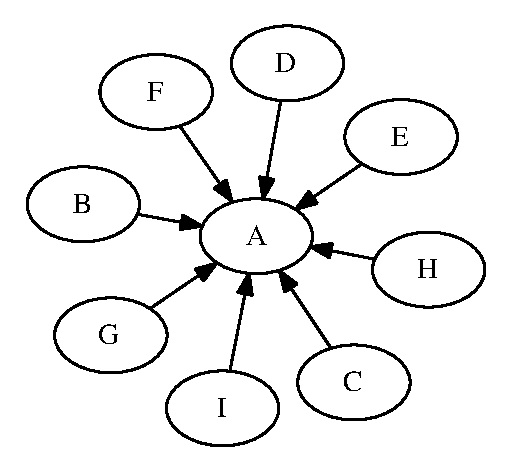
\includegraphics{./imagenes/red_estrella.eps}
    \caption{Red de estrella}
    \label{fig:red_estrella}
  \end{center}
\end{figure}

En la figura \ref{fig:red_estrella} se puede ver un caso en el que el nodo A es una clara celebridad de la red. Este tipo de configuración, llamada red de estrella, es muy poco común en la vida real, pero sirve de ayuda visual para entender a simple vista el concepto de centralidad.

\subsection{Grado de cercanía}

A menudo se puede ver que personas que no tienen mayor influencia aparente en una red son capaces de difundir un mensaje en una gran parte de la red. Esto se debe a que tienen buenas conexiones en la red que les permiten llegar a mas personas, sin que ellos en si sean ``importantes" en la red. Para medir que tan bien o mal posicionado esta un nodo en la red se utiliza el \textbf{grado de cercanía}. Este calculo es bastante caro computacionalmente ya que conlleva una gran cantidad de cálculos.

Los pasos para calcular el grado de cercanía de los nodos de una red son:

\begin{enumerate}
  \item Calcular la ruta mas corta entre todos los pares de nodos posibles, utilizando el algoritmo de Dijkstra, y almacenar estos valores en una tabla.
  \item Para cada nodo de la red:
  \begin{enumerate}
    \item Calcular la distancia promedio con todos los demás nodos.
    \item Dividir el promedio por la distancia mas alta.
    \item Calcular el inverso del valor anterior.
  \end{enumerate}
  \item normalizar cada valor obtenido para obtener valores en el rango de 0-1.
\end{enumerate}

Los nodos que tengan un valor mas cercano a 1 son los que tienen una distancia promedio menor con los nodos de la red, o los que tienen ``\textit{mejores contactos}".

\subsection{Grado de intermediación}

En las redes sociales, suelen formarse grupos mas pequeños que comparten un interés común. Por ejemplo, es mas probable que dos personas que comparten el gusto por los videojuegos interactúen entre si que dos personas que no lo hagan, sin embargo hay casos en los que una persona comparte gustos con diferentes grupos, ayudando a que esta persona se pueda relacionar de manera efectiva con un grupo mas extenso de personas. Estas personas son conocidas como ``puertas frontera" ya que, gracias a ellos, es posible que dos grupos que no tengan nada en común puedan relacionarse entre sí. La medida que ayuda a identificar estos elementos en una red es el \textbf{grado de intermediación}, y consiste en lo siguiente:

\begin{enumerate}
  \item Calcular la ruta mas corta entre todos los pares de nodos posibles, utilizando el algoritmo de Dijkstra, y almacenar estos valores en una tabla.
  \item Para cada nodo n de la red, contar las veces que el nodo n aparece en la lista de rutas mas cortas,
  \item normalizar cada valor obtenido para obtener valores en el rango de 0-1.
\end{enumerate}

Cabe notar que este algoritmo es bastante lento para redes que son muy grandes.

En la figura \ref{fig:bow_tie} se puede ver un claro ejemplo de este fenómeno. Esta red, conocida como la red corbatín (bow-tie en inglés), muestra como el nodo D se encuentra entre 2 grupos de nodos que, de otra manera, no podrían conectarse.

\begin{figure}[!htb]
  \begin{center}
    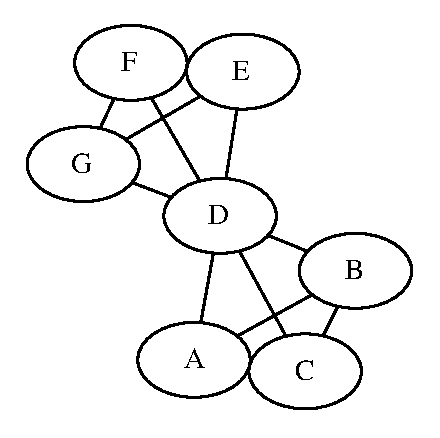
\includegraphics{./imagenes/bow_tie.eps}
    \caption{red corbatín}
    \label{fig:bow_tie}
  \end{center}
\end{figure}

\subsection{Díadas}

Las díadas son la unidad básica de análisis una red social, ya que estas representan la relación entre una y otra persona, esto es, mis amigos, mis seguidores, mis suscriptores, etc. Existen 4 tipos de díadas, representadas en la figura \ref{fig:tipos_diadas}, su uso varia en función del significado de la relación.

\begin{figure}[!htb]
  \begin{center}
      \begin{tabular}{m{3cm}|m{3cm}|m{3cm}|m{3cm}}
        \includegraphics[width=3cm]{./imagenes/diada_1.eps} & 
        \includegraphics[width=3cm]{./imagenes/diada_2.eps} & 
        \includegraphics[width=3cm]{./imagenes/diada_3.eps} & 
        \includegraphics[width=3cm]{./imagenes/diada_4.eps}\\
      \end{tabular}
    \caption{Tipos de diadas asimétricas}
    \label{fig:tipos_diadas}
  \end{center}
\end{figure}

La díada 1 indica que ambos individuos existen en la red, pero todavía no existe ninguna relación entre ellos. Las diadas 2 y 3 muestran una relación unidireccional entre los dos individuos, la única diferencia es el sentido de esa relación. La díada 4, por su parte, es la de mayor interés de las cuatro ya que muestra una relación bidireccional entre los individuos, siendo esta la relación que mayor peso tiene en una red social dado que nos dice que existe un alto grado de reciprocidad en el intercambio de información entra ambos individuos.

\subsection{Tríadas}

Las triadas son básicamente 3 nodos conectados de alguna manera. Al igual que con las diadas, las triadas también pueden ser simétricas o asimétricas, dependiendo estrictamente del contexto en que son utilizadas. Existen 4 tipos de triadas simétricas, ilustradas en la figura \ref{fig:tipos_triadas_simetricas}.

\begin{figure}[!htb]
  \begin{center}
      \begin{tabular}{m{3cm}|m{3cm}|m{3cm}|m{3cm}}
        \includegraphics[width=3cm]{./imagenes/triada_simetrica_1.eps} & 
        \includegraphics[width=3cm]{./imagenes/triada_simetrica_2.eps} & 
        \includegraphics[width=3cm]{./imagenes/triada_simetrica_3.eps} & 
        \includegraphics[width=3cm]{./imagenes/triada_simetrica_4.eps}\\
      \end{tabular}
    \caption{Tipos de triadas simétricas}
    \label{fig:tipos_triadas_simetricas}
  \end{center}
\end{figure}

Por otra parte, existen 16 tipos de triadas asimétricas, numeradas del 1-16. Su uso es mas frecuente ya que de ellas se puede hacer un análisis mas complejo en comparación a las díadas. Cada una de estas triadas recibe un nombre especifico para facilitar su identificación, a continuación se explica como debe leerse ese nombre:

\begin{itemize}
  \item El primer numero representa la cantidad de vértices bidireccionales
  \item El segundo numero representa la cantidad de vértices simples
  \item El tercer numero representa la cantidad de vértices inexistentes
  \item Si una triada se repite, se utiliza una letra extra para determinar que variante es:
  \begin{itemize}
    \item U - Arriba (Up)
    \item D - Abajo (Down)
    \item C - Circulo (Circle)
    \item T - Transitiva (Transitive)
  \end{itemize}
\end{itemize}

En la figura \ref{fig:tipos_triadas_asimetricas} se muestran todas las triadas posibles con su respectivo código asociado.

\begin{figure}[!htb]
  \begin{center}
      \begin{tabular}{m{1.3cm}|m{1.3cm}|m{1.3cm}|m{1.3cm}|m{1.3cm}|m{1.3cm}|m{1.3cm}|m{1.3cm}}
        \includegraphics[width=1.3cm]{./imagenes/triada_003.eps} & 
        \includegraphics[width=1.3cm]{./imagenes/triada_012.eps} & 
        \includegraphics[width=1.3cm]{./imagenes/triada_021C.eps} & 
        \includegraphics[width=1.3cm]{./imagenes/triada_021D.eps} & 
        \includegraphics[width=1.3cm]{./imagenes/triada_021U.eps} & 
        \includegraphics[width=1.3cm]{./imagenes/triada_030C.eps} & 
        \includegraphics[width=1.3cm]{./imagenes/triada_030T.eps} & 
        \includegraphics[width=1.3cm]{./imagenes/triada_102.eps}\\ \hline
        \includegraphics[width=1.3cm]{./imagenes/triada_111D.eps} & 
        \includegraphics[width=1.3cm]{./imagenes/triada_111U.eps} & 
        \includegraphics[width=1.3cm]{./imagenes/triada_120C.eps} & 
        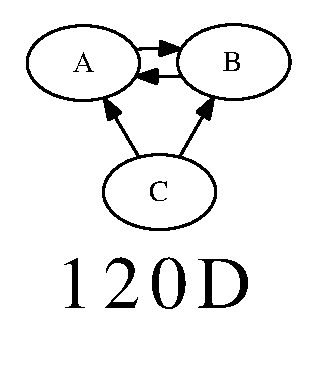
\includegraphics[width=1.3cm]{./imagenes/triada_120D.eps} & 
        \includegraphics[width=1.3cm]{./imagenes/triada_120U.eps} & 
        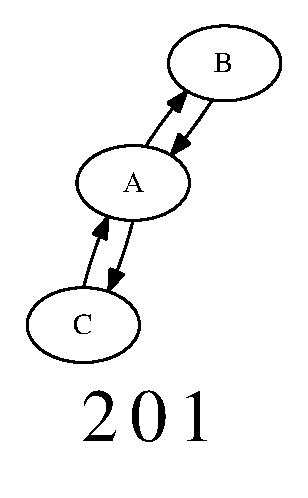
\includegraphics[width=1.3cm]{./imagenes/triada_201.eps} & 
        \includegraphics[width=1.3cm]{./imagenes/triada_210.eps} & 
        \includegraphics[width=1.3cm]{./imagenes/triada_300.eps}\\
      \end{tabular}
    \caption{Tipos de triadas asimétricas}
    \label{fig:tipos_triadas_asimetricas}
  \end{center}
\end{figure}

Gracias a esta discriminación topológica, se puede hacer un análisis mas completo de una red. Este análisis recibe el nombre de \textbf{\textit{Análisis Triadico}}.

\subsection{Análisis Triadico}

Este proceso, que también recibe el nombre de \textbf{Censo Triadico}, consiste en contar la ocurrencia de cada uno de los tipos de triada para cada nodo, y de esa forma determinar el rol que desempeña este nodo en la red. Por ejemplo, un nodo que presente en mayoría triadas del tipo 4, 7 y 11 es un nodo que \textbf{genera contenido}, mientras que si la mayoría de sus triadas son del tipo 5 y/o 10, es un nodo que recibe o \textbf{consume contenidos}.

Adicionalmente se puede hacer el mismo análisis a la red en general, para tener un punto de vista global de la red. En la figura \ref{fig:red_krackhardt} se puede ver una de las redes mas utilizadas en la teoría de redes sociales, la red de Krackhardt-kite. En esta red se pueden ver muchas características de una red social, facilitando el estudio de las mismas. Al hacer el censo a esta red, nos damos cuenta que presenta una gran cantidad de nodos tipo 201, que representan un agujero estructural, y nodos tipo 300, que representan triadas cerradas, esto nos indica que en esta red existen zonas que tienen una gran concentración de nodos interconectados, mientras hay zonas que no se encuentran muy pobladas. Todo esto se puede ver a simple vista en esta red, pero para redes mas grandes puede que represente un problema mayor.

\begin{figure}[!htb]
  \begin{center}
    \includegraphics[width=8cm]{./imagenes/red_krackhardt_kite.eps}
    \caption{Red social de Krackhardt kite}
    \label{fig:red_krackhardt}
  \end{center}
\end{figure}

\subsection{Pandillas}


\input{./Capitulos/4-Marco_teorico/BPMN.tex}

\section{Service-Oriented Architecture (SOA)}
\subsection{Proceso de Análisis y diseño orientados a servicios}

En la etapa de análisis y diseño, el arquitecto de software se reúne con un analista de negocio, el cual diseñará unos servicios candidatos que después se convertirán en los servicios incluidos en los blueprints. Luego de tener los planos, el arquitecto escoge un subconjunto de dichos candidatos a servicios para ser implementados físicamente, dotándolos de algún método para realizar la composición de servicios. En la figura \ref{fig:seis} se muestra el proceso de análisis y diseño orientado a servicios.

\begin{figure}[!htb]
  \begin{center}
    \includegraphics[width=11cm]{./imagenes/6.png}
    \caption{proceso de análisis y diseño orientado a servicios}
    \label{fig:seis}
    \textbf{Fuente:}  \cite{soa_principles}
  \end{center}
\end{figure}

\subsection{Metas y beneficios de la computación orientada a servicios }

Las metas y los beneficios que trae la implementación de la computación orientada a servicios en una organización son:

\begin{itemize}
  \item \textbf{Incremento de la interoperabilidad intrínseca}: Es una meta de la computación orientada a servicios ya que la composición de servicios requiere que, sin necesidad de integrar un servicio con el otro, estos puedan intercambiar información para desarrollar la funcionalidad a la que han sido inscritos. Aplicando principios de diseño orientados a servicios, así como también estándares de diseño orientados a servicios, se logra el incremento de la interoperabilidad intrínseca.
  \item \textbf{Federación incrementada}: Un entorno de TI federado es aquel en el cual los recursos y aplicaciones se manejan y gobiernan con autonomía y por sí mismos. En el ámbito de la orientación a servicios, cada servicio puede tener su propia implementación independiente y aun así comunicarse. Esto se logra por medio de una especial atención a los estándares de diseño.
  \item \textbf{Incremento de opciones en la escogencia de proveedores de servicios}: Como la federación en la computación orientada a servicios es una meta, la escogencia de proveedores de servicios diferentes es un beneficio ya que la composición de servicios puede ser lograda sin importar que proveedor provea de un servicio específico.
  \item \textbf{Incremento de la alineación entre el negocio y las tecnologías}: Ya que en el proceso de diseño actúan tanto el analista de negocio como el arquitecto de software, la alineación entre negocio y tecnologías es incrementada. La reconfiguración en la composición de servicios, además, provee alineación extra al poder cambiar el proceso de negocio y la composición de los servicios al mismo tiempo.
  \item \textbf{ROI}: Al hacerse inventarios de servicios y, además, ser los servicios reutilizables a lo largo del tiempo y compuestos de diferente forma gracias a la composición de servicios, se da una relación costo/beneficio más baja que con otros paradigmas usados.
  \item \textbf{Agilidad organizacional incrementada}: Debido a la orientación a servicios, se hace una composición rápida de los servicios que se tengan y se crean los que se necesiten para agilizar el proceso del departamento de TI y así agilizar los procesos subyacentes.
  \item \textbf{Reducción de cargas al departamento TI}: Debido a la agilidad organizacional cuando es aplicada la orientación a servicios, son reducidos costos operacionales (tiempo u otros recursos) y el departamento de TI adquiere un papel activo en el sector estratégico.
\end{itemize}


\section{Estado del arte} \label{cap:estado_arte}
\subsection{UX - Análisis}
Los servicios de redes sociales (SNS por sus siglas en ingles: Social Network Services) como Facebook, LinkedIn, Twitter, SportTracker o Xportia, ofrecen servicios para la gestión de la OSN de cada usuario que acceda a estas aplicaciones. Según un estudio hecho para medir la experiencia de usuario (UX por sus siglas en ingles: User eXperience) en los SNS, se encontraron 8 categorías que son críticas a la hora de diseñar una SNS y son:

\begin{enumerate}
  \item Self-expresion: Capacidad que tengan las OSN de compartir contenido relacionado a la vida real de los usuarios tal como lo pueden ser las fotos, los videos, los comentarios o las comunicaciones directas.
  \item Reciprocity: Interacción bilateral en tiempo real, es decir, interacción instantánea con uno o varios individuales en la OSN (por ejemplo, por medio de los servicios de mensajería instantánea).
  \item Learning: La información recibida por medio de la OSN debe poder ser utilizada en pro del desarrollo cognitivo del individual; debe existir información útil al individual que usa la OSN.
  \item Curiosity: El contenido de la OSN debe ser interesante para quien la utiliza.
  \item Suitability of functionality: Se refiere a cuán ``utilizable'' es una funcionalidad.
  \item Suitability of content: La calidad y exactitud de la información que en la OSN reside debe ser suficiente para el individual perteneciente a ella.
  \item Completeness of the user network: Los individuales deben querer pertenecer a la red social y buscar eficientemente a otros individuales para poder formar lazos con ellos y hacer crecer su red social.
  \item Trust and privacy: Confianza en los servicios de las OSN, así como también la capacidad que tiene el usuario de gestionar la privacidad del contenido que comparte en dicha OSN. \cite{social_experience}

Cada uno de las categorías nombradas hace parte de los factores que impulsan la utilización de los SNS para la gestión de las OSN de las personas. 
\end{enumerate}

\subsection{Factor distancia en la formación de las redes sociales}

La formación de redes sociales (tanto fuera de línea como en línea) es afecta por la distancia entre cada individual y el posible tipo de enlace que los uniría. En \cite{evolution} se hizo un estudio acerca de la formación de lazos, la formación de triadas entre individuales de una red social basada en la inscripción localizaciones recomendadas y frecuentadas por los usuarios, teniendo como parámetros ``la edad'' o tiempo de vinculación del individual a la red social, el grado de cada individual (número de conexiones que tiene un individual a otro) y la localización de cada individual en la red social. También se analizó cómo afectaba la creación de nuevos lazos con la movilidad del usuario (el desplazamiento por lugares geográficos distintos). En conclusión, se verificó que la formación de lazos depende proporcionalmente de la edad y del grado del individual y es inversamente proporcional a la distancia que a cada individual y que la formación de lazos puede modelarse con solo dos de los tres factores (el grado y la distancia); en cuanto a la formación de triadas, se verificó que ésta depende de las características sociales de la red, tomando énfasis en los individuales compartidos entre los posibles individuales formadores de triadas. Además, en cuanto a la creación de nuevos lazos teniendo en cuenta los lugares visitados por cada usuario de la red social, se presenta un patrón: Los usuarios escogen un lugar popular para visitar y, posteriormente, dirimen con que usuario crear un lazo teniendo en cuenta su popularidad y que frecuente los mismos lugares siempre.

\begin{landscape}
  
\begin{table}
  \caption{Comparacion de redes, parte 1}
  \label{tab:comparacion_redes_1}

  \begin{center}
  
  \resizebox{20cm}{!}{
  \begin{tabular}{|p{5cm}|llll|}
    \hline
    Fun\textbackslash Red social & \multicolumn{1}{c}{Sportfactor} & \multicolumn{1}{c}{Deportesreunidos} & \multicolumn{1}{c}{Mybestplay} & \multicolumn{1}{c|}{Subetudeporte} \\ 
    \hline
    Gestión de foros & \multicolumn{1}{c}{} & \multicolumn{1}{c}{Si} & \multicolumn{1}{c}{} & \multicolumn{1}{c|}{Si} \\ 
    \hline
    Gestión de encuentros deportivos & \multicolumn{1}{c}{} & \multicolumn{1}{c}{- Organización de eventos} & \multicolumn{1}{c}{} & \multicolumn{1}{c|}{} \\ 
     & \multicolumn{1}{c}{} & \multicolumn{1}{c}{-Encuentros deportivos informales} & \multicolumn{1}{c}{} & \multicolumn{1}{c|}{} \\ 
     & \multicolumn{1}{c}{} & \multicolumn{1}{c}{} & \multicolumn{1}{c}{} & \multicolumn{1}{c|}{} \\ 
    \hline
    Creación de grupos & \multicolumn{1}{c}{} & \multicolumn{1}{c}{Si} & \multicolumn{1}{c}{} & \multicolumn{1}{c|}{} \\ 
    \hline
    Manejo de torneos & \multicolumn{1}{c}{} & \multicolumn{1}{c}{- Organización y difusión} & \multicolumn{1}{c}{} & \multicolumn{1}{c|}{} \\ 
    \hline
    Difusión info. Deportiva & \multicolumn{1}{c}{-RSS de noticias} & \multicolumn{1}{c}{- Blog propio} & \multicolumn{1}{c}{-Difusión de eventos} & \multicolumn{1}{c|}{- Gestión de blogs} \\ 
     & \multicolumn{1}{c}{} & \multicolumn{1}{c}{} & \multicolumn{1}{c}{-Blog propio} & \multicolumn{1}{c|}{} \\ 
    \hline
    Serv. self-expression & \multicolumn{1}{c}{} & \multicolumn{1}{c}{-Difusión de multimedia} & \multicolumn{1}{c}{-Difusión de multimedia } & \multicolumn{1}{c|}{-Difusión de multimedia} \\ 
     & \multicolumn{1}{c}{} & \multicolumn{1}{c}{} & \multicolumn{1}{c}{} & \multicolumn{1}{c|}{} \\ 
    \hline
    Sistema estadístico & \multicolumn{1}{c}{-Medición de avance en} & \multicolumn{1}{c}{- Sistemas de estadísticas para cada servicio} & \multicolumn{1}{c}{} & \multicolumn{1}{c|}{} \\ 
     & \multicolumn{1}{c}{ estadísticas del deporte practicado} & \multicolumn{1}{c}{} & \multicolumn{1}{c}{} & \multicolumn{1}{c|}{} \\ 
    \hline
    Gestión de transversales & \multicolumn{1}{c}{-Trainner personales} & \multicolumn{1}{c}{} & \multicolumn{1}{c}{} & \multicolumn{1}{c|}{} \\ 
     & \multicolumn{1}{c}{-Guías de nutrición} & \multicolumn{1}{c}{} & \multicolumn{1}{c}{} & \multicolumn{1}{c|}{} \\ 
     & \multicolumn{1}{c}{- Catalogo de lesiones y fisioterapia} & \multicolumn{1}{c}{} & \multicolumn{1}{c}{} & \multicolumn{1}{c|}{} \\ 
    \hline
    Servicios deportivos & \multicolumn{1}{c}{-Guía deportiva (shops, restaurantes, etc.)} & \multicolumn{1}{c}{} & \multicolumn{1}{c}{} & \multicolumn{1}{c|}{} \\ 
     & \multicolumn{1}{c}{} & \multicolumn{1}{c}{} & \multicolumn{1}{c}{} & \multicolumn{1}{c|}{} \\ 
    \hline
    Soporte multi-deporte & \multicolumn{1}{c}{Si} & \multicolumn{1}{c}{Si} & \multicolumn{1}{c}{Solo deportes en equipo} & \multicolumn{1}{c|}{Si} \\ 
    \hline
    Gestión de tipos de usu. & \multicolumn{1}{c}{} & \multicolumn{1}{c}{- Equipos } & \multicolumn{1}{c}{Si} & \multicolumn{1}{c|}{} \\ 
     & \multicolumn{1}{c}{} & \multicolumn{1}{c}{- Clubes} & \multicolumn{1}{c}{} & \multicolumn{1}{c|}{} \\ 
     & \multicolumn{1}{c}{} & \multicolumn{1}{c}{-Centros deportivos} & \multicolumn{1}{c}{} & \multicolumn{1}{c|}{} \\ 
    \hline
    Gestión de sponsors & \multicolumn{1}{c}{} & \multicolumn{1}{c}{} & \multicolumn{1}{c}{Si} & \multicolumn{1}{c|}{} \\ 
    \hline
    Gestión del conocimiento & \multicolumn{1}{c}{} & \multicolumn{1}{c}{} & \multicolumn{1}{c}{} & \multicolumn{1}{c|}{} \\ 
    \hline
    Gestión de geolocaliza. & \multicolumn{1}{c}{} & \multicolumn{1}{c}{} & \multicolumn{1}{c}{} & \multicolumn{1}{c|}{} \\ 
     & \multicolumn{1}{c}{} & \multicolumn{1}{c}{} & \multicolumn{1}{c}{} & \multicolumn{1}{c|}{} \\ 
    \hline
    Soporte móvil & \multicolumn{1}{c}{} & \multicolumn{1}{c}{} & \multicolumn{1}{c}{} & \multicolumn{1}{c|}{} \\ 
     & \multicolumn{1}{c}{} & \multicolumn{1}{c}{} & \multicolumn{1}{c}{} & \multicolumn{1}{c|}{} \\ 
    \hline
    Conexión con otros SNS & \multicolumn{1}{c}{} & \multicolumn{1}{c}{} & \multicolumn{1}{c}{} & \multicolumn{1}{c|}{} \\ 
     & \multicolumn{1}{c}{} & \multicolumn{1}{c}{} & \multicolumn{1}{c}{} & \multicolumn{1}{c|}{} \\ 
    \hline
  \end{tabular}
  }
    \end{center}
\end{table}
  
  \newpage
  
  \begin{table}
  \caption{Comparacion de redes, parte 2}
  \label{tab:comparacion_redes_2}

  \begin{center}
  
  \resizebox{20cm}{!}{
    \begin{tabular}{|p{4cm}|p{9cm}p{7cm}p{7cm}|}
\hline
Fun\textbackslash Red social & Sporttia & Amatteur & Fitivity  \\ 
\hline
Gestión de foros &  &  &  \\ 
\hline
Gestión de encuentros deportivos & - Organización de eventos en centros deportivos & - Publicación o búsqueda de eventos deportivos & -Basado en geolocalización \\ 
 & - Gestión de jugadores &  &  \\ 
 & -Gestión de características del partido &  &  \\ 
\hline
Creación de grupos &  &  &  \\ 
\hline
Manejo de torneos &  &  &  \\ 
\hline
Difusión info. Deportiva &  &  &  \\ 
 &  &  &  \\ 
\hline
Serv. self-expression &  & -Difusión de multimedia &  \\ 
 &  &  &  \\ 
\hline
Sistema estadístico &  &  &  \\ 
 &  &  &  \\ 
\hline
Gestión de transversales &  &  &  \\ 
 &  &  &  \\ 
 &  &  &  \\ 
\hline
Servicios deportivos & -Alquiler de centros deportivos & - Servicios de compra y venta de artículos deportivos &  \\ 
 &  &  &  \\ 
\hline
Soporte multi-deporte & Si & Si & Si \\ 
\hline
Gestión de tipos de usu. & -Deportista -Centro deportivo & -Deportista  &  \\ 
 &  & -Equipo &  \\ 
 &  &  -Organización &  \\ 
\hline
Gestión de sponsors &  & -Promoción como deportista, equipo u organización &  \\ 
\hline
Gestión del conocimiento & - Clases virtuales &  &  \\ 
\hline
Gestión de geolocaliza. &  & Si & Si \\ 
 &  &  &  \\ 
\hline
Soporte móvil &  &  & -Android \\ 
 &  &  & -IOS \\ 
\hline
Conexión con otros SNS &  &  &  \\ 
\hline
\multicolumn{1}{l}{} &  &  & \multicolumn{1}{l}{} \\ 
\end{tabular}
  }
      \end{center}
\end{table}

\newpage

\begin{table}
  \caption{Comparacion de redes, parte 3}
  \label{tab:comparacion_redes_3}

  \begin{center}
  \resizebox{20cm}{!}{
  \begin{tabular}{|p{4cm}|p{7cm}p{6cm}p{9cm}|}
\hline
Fun\textbackslash Red social & Bkool & Deportmeet & Sportsnak \\ 
\hline
Gestión de foros &  &  & - Foros con profesionales (managers, coaches, teams) \\ 
 &  &  & - Ofrece posibilidad al usuario de ser moderador de foros \\ 
\hline
Gestión de encuentros deportivos & - Creación de eventos deportivos (solo o con amigos) &  - Gestión de eventos deportivos & - Manejo de eventos deportivos \\ 
 & - Gestión de ``retos'' &  &  \\ 
\hline
Gestión de grupos & Si &  &  \\ 
\hline
Manejo de torneos &  &  &  \\ 
\hline
Difusión info. Deportiva & - Gestión de información de ligas & - Artículos de profesionales & -Asociación con blogs deportivos \\ 
 &  &  & - Manejo de ``live scores'' \\ 
\hline
Serv. self-expression & -Subida de texto plano & -Difusión de multimedia & - Manejo contenido plano y multimedia \\ 
 & -Difusión de multimedia &  & - Uso de mensajería instantánea \\ 
\hline
Sistema estadístico & - Estadísticas de deportista & - Gestión del nivel del deportista &  \\ 
 &  & -Manejo de perfiles de usuario &  \\ 
\hline
Gestión de transversales &  & -Foros de nutrición &  \\ 
\hline
Servicios deportivos &  & - Venta de artículos deportivos & - Módulos para negociantes en temas de deporte \\ 
 &  &  & - Manejo de ofertas en ofrecimiento de instalaciones deportivas \\ 
 &  &  & -- Herramientas para hacer ``boost'' a negociantes (bussiness member) \\ 
\hline
Soporte multi-deporte & Deportes de ruta & Si & Si \\ 
 &  &  &  \\ 
\hline
Gestión de tipos de usu. &  &  & -Public member \\ 
 &  &  & -Club member \\ 
 &  &  & -Bussiness member \\ 
\hline
Gestión de sponsors &  &  & - Manejo de ``sponsorship'' \\ 
\hline
Gestión del conocimiento &  &  &  \\ 
 &  &  &  \\ 
\hline
Gestión de geolocaliza. & - Posibilidad de grabar trazados & - Localización de eventos & - Geolocalización de actividad deportiva cercana a un punto \\ 
 & (deportes de ruta) &  &  \\ 
\hline
Soporte móvil & -Android &  &  \\ 
 & -IOS &  &  \\ 
\hline
Conexión con otros SNS & -Facebook &  &  \\ 
 & -twitter &  &  \\ 
\hline
\end{tabular}
}
  
  \end{center}
\end{table}

\newpage

\begin{table}
  \caption{Comparacion de redes, parte 4}
  \label{tab:comparacion_redes_4}

  \begin{center}
    \resizebox{20cm}{!}{
    \begin{tabular}{|p{5cm}|lll|}
\hline
Fun\textbackslash Red social & Huddlers & Yoyde & Timpik \\ 
\hline
Gestión de foros &  &  &  \\ 
 &  &  &  \\ 
\hline
Gestión de encuentros deportivos & - Organización de eventos deportivos & - Manejo de eventos deportivos & - Manejo de eventos deportivos \\ 
 &  &  &  \\ 
\hline
Gestión de grupos &  &  &  \\ 
 &  &  &  \\ 
\hline
Manejo de torneos &  & Si &  \\ 
\hline
Difusión info. Deportiva &  & - Manejo de blogs &  \\ 
 &  &  &  \\ 
\hline
Serv. self-expression &  & -Manejo de ``muro'' & - Manejo de ``muro''  \\ 
 &  &  & -Gestión de mensajería \\ 
\hline
Sistema estadístico &  &  &  \\ 
 &  &  &  \\ 
 &  &  &  \\ 
\hline
Gestión de transversales &  &  &  \\ 
\hline
Servicios deportivos &  &  &  \\ 
\hline
Soporte multi-deporte & Si & Si & Si \\ 
 &  &  &  \\ 
\hline
Gestión de tipos de usu. &  & -Club deportivo & - Manejo de perfil deportivo \\ 
 &  & -Deportista &  \\ 
\hline
Gestión de sponsors &  &  &  \\ 
\hline
Gestión del conocimiento &  &  &  \\ 
 &  &  &  \\ 
\hline
Gestión de geolocaliza. & - Funcionalidad ``jugando en'' & - Manejo de escenarios deportivos &  \\ 
 &  & - Manejo de ``rutas'' &  \\ 
\hline
Soporte móvil & -IOS &  & -Android \\ 
\hline
Conexión con otros SNS &  &  &  \\ 
\hline
\end{tabular}
}
  
  \end{center}
\end{table}

\begin{table}
  \caption{Comparacion de redes, parte 5}
  \label{tab:comparacion_redes_5}

  \begin{center}
  \resizebox{20cm}{!}{
    \begin{tabular}{|p{4cm}|p{7cm}p{7cm}p{8cm}|}
\hline
Fun\textbackslash Red social & Socialsports & Strava & Ineftos \\ 
\hline
Gestión de foros &  &  & Si \\ 
\hline
Gestión de encuentros deportivos & - Organizador de eventos deportivos & - Manejo de desafíos (challenges) & - Organización de eventos \\ 
\hline
Gestión de grupos &  &  & Si \\ 
\hline
Manejo de torneos &  &  &  \\ 
\hline
Difusión info. Deportiva &  &  & - Manejo de blogs para estudiantes \\ 
\hline
Serv. self-expression & - Manejo de multimedia &  & - Manejo de mensajería \\ 
 &  &  & - Manejo de ``muro'' \\ 
 &  &  & - Manejo de multimedia \\ 
\hline
Sistema estadístico &  & - Gestión de estadísticas del atleta & - Utiliza mecanismo de encuestas para autorregularse \\ 
 &  & - Gestión de ``follows'' a otros deportistas para comparación de estadísticas (competencia) & - Gestión de foros: Estadísticas de foro \\ 
\hline
Gestión de transversales &  &  &  \\ 
\hline
Servicios deportivos & - Evaluación de la comunidad sobre los prestadores de servicio &  &  \\ 
\hline
Soporte multi-deporte & Si & Monodeporte (ciclomontañismo) & Si \\ 
\hline
Gestión de tipos de usu. & - Manejo de perfil de deportista (deportes practicados, lugares frecuentados, horarios frecuentados) &  & - Manejo de usuarios (profesores, alumnos, entidades sin ánimo de lucro) \\ 
 & - Manejo de usuarios (prestadores de servicio y deportistas) &  &  \\ 
\hline
Gestión de sponsors &  &  &  \\ 
\hline
Gestión del conocimiento &  & - Encuentro de consejos deportivos & - ``Social learning'' \\ 
\hline
Gestión de geolocaliza. &  & - Gestión de trazados logrados &  \\ 
 &  & - Gestión de trazados &  \\ 
\hline
Soporte móvil &  & -Android &  \\ 
\hline
Conexión con otros SNS &  &  &  \\ 
\hline
\end{tabular}
  }
  \end{center}
\end{table}

\end{landscape}


  
  \chapter{Marco legal}
  En cuanto al trabajo con datos, las leyes creadas en Colombia para la protección y manejo de estos son:

\begin{itemize}
  \item Constitución Nacional, en el artículo 15, del derecho a la intimidad y al buen nombre. Debido al carácter que tiene un SNS, es posible que una persona pueda degradar el buen nombre de otra, así como violar su intimidad.
  \item Código penal, artículos 220 y 221, acerca de la injuria y la calumnia. Similar al anterior punto, casos de injuria y calumnia corresponden a una mala utilización de un SNS, en aras de provocar daño a otra persona.
  \item Ley 23 de 1982, de los derechos de autor. Debido a los espacios de difusión de información que se presentan en un SNS, esta ley entra a escena. Además, las normas de derechos de autor también califican dentro de cualquier trabajo de software que se haga.
  \item Ley 527 de 1999, la cual reglamenta el manejo de mercancías en el comercio electrónico, la utilización de firmas digitales, la reglamentación para certificados expedidos de forma electrónica con firma digital, el manejo de los mensajes de datos y las disposiciones de la Superintendencia de Industria y Comercio. Debido a que este SNS puede llegar a ser utilizado con carácter comercial, esta ley aplica en la creación del SNS.
  \item Ley 663 de 2000, artículo 91, de las obligaciones de presentar registro mercantíl para los sitios web que tengan carácter comercial. De igual manera que el anterior, algunas de las funcionalidades que se pudieran llegar a implementar, pudiesen llegar a ser con un carácter netamente comercial, por lo que es necesario estar al tanto de esta ley y artículo en particular.
  \item Ley 1266 de 2008, el cual reglamenta el tratamiento de datos personales en bases de datos personales, haciendo énfasis en las financieras y comerciales. Debido a que los SNS manejan datos personales de sus usuarios y, a su vez, puede llegar a incluir funcionalidades con carácter comercial, es debido tener en cuenta la ley.
  \item Ley 1273 de 2009, la cual reglamenta el uso de la información y los sistemas de información en contra de la violación de la confidencialidad, la integridad y la disponibilidad de los datos y los sistemas de información, así como también hurtos informáticos. Debido a que ésta ley reglamenta la utilización de la información que tengan en su poder los manejadores de un sistema informático, es menester conocer dicha ley.
  \item Ley 1480 de 2011, la cual reglamenta los derechos y deberes tanto de consumidores como de productores en todos los sectores económicos, aplicándose ésta a los productos tanto importados como nacionales. Debido a que el SNS puede tener funcionalidades de carácter comercial, es necesario saber que leyes aplican a consumidores y productores o prestadores de servicio que la pudieren utilizar.
  \item Resolución 3066 de 2011, la cual busca proteger los derechos de los usuarios de servicios de comunicaciones en los cuales se establece también los derechos sobre los servicios adquiridos en telecomunicaciones. Debido a que el usuario del SNS pudiera llegar a obtener servicios en telecomunicaciones (por ejemplo, la conexión del SNS con la línea telefónica para algún tipo de acción), es necesario conocerla para saber cuando si y cuando no se debe juzgar una posible violación de los derechos de los usuarios de parte de los creadores y de aquellos que pudieran llegar a mantener el SNS.
  \item Ley 1581 de 2012, de disposiciones acerca del tratamiento de datos personales, haciendo énfasis en las políticas de manejo y en las auditorías. Debido a que el SNS tratará con algunos datos personales de sus usuarios, se debe prestar atención a que políticas de manejo de datos personales existen, una de ellas, en esta ley.
  \item Decreto 1377 de 2013, el cual dictamina las políticas de protección y tratamiento de datos personales. Igual que el anterior, se hace necesario conocer que decretos dictaminan la utilización de datos personales por parte de los usuarios del SNS.
\end{itemize}

Lo anterior es tomado de \textit{Legislación en internet} \cite{leg_int}.

Además, se deben tener en cuenta las condiciones de servicio que Google ha impuesto para las aplicaciones desarrolladas para Android, así como también las condiciones aplicadas a la utilización de dichas aplicaciones. Cada una de estas políticas desarrolladas para Android involucra el análisis del entorno legal que enmarca al SNS, debido a que la tecnología a utilizar será principalmente basa en Android. Entonces, se han de tener en cuenta las siguientes condiciones de servicio:

\begin{itemize}
  \item Google Play Terms of Service, el cual dictamina las pautas de uso de Google Play por parte del usuario final, así como también las facultades que tiene Google sobre la información y las aplicaciones instaladas en el dispositivo de un usuario.
  \item Developer Distribution Agreement, el cual reglamenta el uso que el desarrollador o distribuidor de aplicaciones hace de Google Play. Habla acerca del licenciamiento, el manejo de precios y pagos, el manejo de marcas y publicidad y la dada de baja de las aplicaciones de Google Play.
  \item Google Play Business and Program Policies, el cual reglamenta cómo deben ser utilizadas las aplicaciones en cuanto a la información publicada en las mismas y además quien puede utilizar Google Play. Además, reglamenta la devolución, compra, descarga y soporte de productos (aplicaciones) en Google Play.
  \item Developer Content Policy, el cual establece las políticas de contenido y publicidad que puede poner un desarrollador en sus aplicaciones.
\end{itemize}

  
  \chapter{Metodología}
  
Equipo SCRUM:

\begin{itemize}
  \item Product Owner \\
	Doctor Carlos Enrique Montenegro

  \item Developement Team
	\begin{itemize}
	  \item Nicolás Mauricio García Garzón
	  \item Luis Felipe Gonzalez Moreno
	\end{itemize}

  \item Scrum Master \\
	Profesor Alejandro Daza
\end{itemize}

Actividades de cada Sprint (15 días máximo):
  
\begin{itemize}
  \item Sprint Planning (4 horas máximo)\\
  Se realizó una reunión con el Scrum Master al inicio de cada iteración. En esta reunión se discutió el desempeño del Sprint anterior, los servicios/funcionalidades que hacían falta para completar el prototipo, y que servicios debían ser realizados en la iteración.
	\begin{itemize}
	  \item ¿Qué se hizo en cada sprint? \\
	    Con base a los servicios y casos de uso de negocio encontrados, se determino que podía ser desarrollado por el developement team en cada iteración del prototipo.
	  \item ¿Como se llevará a cabo este trabajo? \\
	    Se dividieron los servicios propuestos como parte del Sprint entre los desarrolladores y se compartieron las expectativas que debe cumplir cada servicio para que sea aceptado en el desarrollo.
	\end{itemize}
  \item Daily Scrum (15 minutos máximo)[Solo participa el developement team] \\
  Partiendo de los items asignados a cada desarrollador, se dividieron en tareas aún mas pequeñas que sirvieron como ruta para cumplir con el Sprint Goal. Se respondieron las siguientes preguntas para llevar un seguimiento continuo del desarrollo del prototipo:
	\begin{itemize}
	  \item ¿Qué se hizo ayer que ayudó al developement team para cumplir el Sprint goal?
	  \item ¿Qué se va a hacer hoy para ayudar al developement team a cumplir el Sprint goal?
	  \item ¿Hay algún impedimento para que el developement team cumpla el Sprint goal?
	\end{itemize}
  \item Sprint Review (2 horas máximo) \\
  Se realizó al final de cada Sprint. Se mostro qué se hizo en el sprint con respecto a las tareas propuestas desde el inicio del mismo. Las actividades básicas que se llevaron a cabo fueron:
	\begin{itemize}
	  \item Socializar la experiencia en el sprint, que problemas ocurrieron y cómo se solucionaron.
	  \item Exponer los diferentes elementos que fueron construidos y se resuelven preguntas acerca de los mismos.
	  \item Proponer que puede hacerse en el siguiente Sprint basados en la experiencia del actual.
	  \item Revisar cómo el cambio en el entorno pudo cambiar las prioridades en el trabajo del equipo.
	\end{itemize}
  \item Sprint Retrospective
  \begin{itemize}
    \item Se tomaron las experiencias de cada sprint para formular sugerencias que ayudaron a mejorar los siguientes.

  \end{itemize}
\end{itemize}

A continuación, se presenta el product backlog inicial del proyecto.

\begin{table}[h]
  \caption{Product backlog inicial}
  \label{tab:backlog}

  \begin{center}
    \resizebox{15cm}{!}{
      \begin{tabular}{|l|l|l|}
        \hline
        Tarea & Días & Condición de aprobación \\ 
        \hline
        \hline
        Levantamiento de requerimientos & 2 & Satisfacción de todos los \\ 
        
         &  & requerimientos para la red social \\ 
        
        Definición de requerimientos funcionales y no funcionales & 2 & Modularización y descripción total de  \\ 
        
         &  & todos los requerimientos \\ 
        
        Investigación de tecnologías existentes & 6 & Escogencia de las tecnologías a utilizar \\ 
        
         &  & para implementar la red social \\ 
        
        Diseño de casos de uso & 5 & Cubrimiento de todos los requerimientos identificados \\ 
        
        Refinamiento de requerimientos & 1 & Trazabilidad entre casos de uso y requerimientos \\ 
        
        Identificación de servicios candidatos & 1 & Cubrimiento de todos los requerimientos identificados \\ 
        
        Diseño de blueprints de servicios & 4 & Cubrimiento de todos los servicios candidatos \\ 
        
        Escogencia de servicios a ser implementados & 1 & Viabilidad de un prototipo funcional \\ 
        
        Composición estática de servicios & 5 & Concordancia entre los casos de uso  \\ 
        
         &  & y la composición de servicios \\ 
        
        
        Diseño de base de datos & 6 & Diseño que cubra los servicios a ser implementados \\ 
        
         &  &  y requerimientos no funcionales \\ 
        
        Diseño de interfaz gráfica de usuario & 4 & Cubrimiento de los servicios y casos de uso a ser implementados \\ 
        
         &  &  a ser implementados \\ 
        
        Refinamiento de casos de uso & 1 & Trazabilidad \\ 
        
        Refinamiento de blueprints de servicios & 1 & Trazabilidad \\ 
        
        Refinamiento de servicios a ser implementados & 1 & Trazabilidad \\ 
        
        Refinamiento de composición estática de servicios & 1 & Trazabilidad \\ 
        
        Construcción de la interfaz de usuario & 20 & Navegabilidad sobre las funcionalidades a ser implementadas \\ 
        
        y refinamiento de interfaz de usuario &  &  \\ 
        
        Construcción de los servicios a ser  & 35 & Construcción de prototipo funcional sin fallas \\ 
        
        implementados y refinamiento de modelos &  & detectadas en tiempo de desarrollo \\ 
        
        Pruebas del prototipo por parte del equipo de desarrollo & 2 & Prototipo sin fallas detectables en sus funcionalidades \\ 
        
        Pruebas del prototipo por parte del usuario final & 7 & Prototipo aceptado por el usuario final en al menos un 70\% \\
        \hline

        \end{tabular}
    }
    \textbf{Fuente:} Autores
  \end{center}
\end{table}

  
  \chapter{Cronograma}
  \input{./Capitulos/Cronograma/Cronograma.tex}
  
  \chapter{Costos}
  \label{chap:costos}
  \section{Recursos de Hardware}
En la tabla \ref{tab:rec_hardware} se muestran los costos estimados en los que se incurrirá para el desarrollo del proyecto con respecto a recursos de hardware.
  \begin{table}[!htb]
    \caption{Recursos de hardware}
    \label{tab:rec_hardware}
    \begin{center}
    \resizebox{11cm}{!}{
        \begin{tabular}{|c|p{5cm}|c|c|c|}
          \hline
          Recurso & Descripción & Cantidad & Costo Unitario & Total\\
          \hline \hline
          Computador & Core i7 2670QM, 1TB de Disco Duro, 10GB de memoria RAM & 1 & \$145.000/mes & \$870.000\\
          \hline
          Tablet & Google Nexus 10 & 1 & \$75.000/mes & \$450.000\\
          \hline
          Smartphone & Samsung Galaxy S3 Mini & 1 & \$40.000/mes & \$240.000\\
          \hline
          Smartphone & Huaweii Y300-0151 & 1 & \$30.000/mes & \$180.000\\
          \hline
		  Computador & Core i7 4500, 1TB de Disco Duro, 8GB de memoria RAM & 1 & \$145.000/mes & \$870.000\\
		  \hline
          Computador & Intel Pentium G2020 @ 2.90GHz 2 nucleos, 320GB de disco duro, 4GB de memoria RAM & 1 & \$120.000/mes & \$720.000 \\
          \hline
        \end{tabular}
    } \\
    \textbf{Fuente}: Cotización con empresa \textbf{RentaSistemas} - www.rentasistemas.com
    \end{center}
  \end{table}

  \section{Recursos de Software}
En la tabla \ref{tab:rec_software} se muestran los costos estimados en los que se incurrirá para el desarrollo del proyecto con respecto a recursos de software.
  \begin{table}[!htb]
    \caption{Recursos de software}
    \label{tab:rec_software}
    \begin{center}
    \resizebox{10cm}{!}{
          \begin{tabular}{|p{5cm}|p{7cm}|}
          \hline
          Recurso & Descripción\\
          \hline \hline
          Debian Versión 7.4 (wheezy),32-bit & Sistema operativo en el que se realizará el desarrollo \\
          \hline
          Eclipse IDE & Entorno de desarrollo de código abierto \\
          \hline
          Android Studio & IDE proporcionado por Gooogle que brinda un entorno de desarrollo para construir aplicaciones Android \\
          \hline
          Android 4.0 Ice Cream & API para el desarrollo de aplicaciones móviles para Android 4.0 y superiores \\
          \hline
          Enterprise Architect 11 & Herramienta para modelado de software (en nuestro caso, UML)  \\
		  \hline
          Archi 3.0 & Herramienta libre y gratuita para crear modelos en el estándar Archimate \\
		  \hline
		  Evolus Pencil 2.0.5 & Herramienta libre para el diseño de interfaces gráficas de usuario \\
		  \hline
		  Neo4j 2.1.7 & Motor de base de datos orientado a grafos \\
		  \hline          
          WildFly 8.2.0 & Servidor de aplicaciones libre y gratuito que se utiliza como backend de la aplicación \\
          \hline
        \end{tabular}
    } \\
    \textbf{Fuente:} Autores \\
      \footnotesize \textbf{Nota:} Los costos incurridos en instalación, configuración o capacitaciones están cubiertos en el salario del developement team.
    \end{center}
  \end{table} 

  \input{./Capitulos/Recursos/Humanos.tex}
  \section{Recursos misceláneos}
En la tabla \ref{tab:rec_miscelanea} se muestran los costos estimados en los que se incurrirá para el desarrollo del proyecto con respecto a recursos de misceláneos.
  \begin{table}[!htb]
    \caption{Recursos misceláneos}
    \label{tab:rec_miscelanea}
    \begin{center}
    \resizebox{11cm}{!}{
      \begin{tabular}{|l|l|l|l|}
        \hline
        Concepto           & Cantidad   & Valor mensual & Valor total \\
        \hline
        \hline
        Papelería          & N/A        & \$10.000      & \$60.000    \\
        Servicios Públicos & 3          & \$180.000     & \$1'080.000 \\
        Transporte         & 2 personas & \$144.000     & \$864.000  \\
        \hline
      \end{tabular}
    }
    \end{center}
  \end{table}

    \clearpage
\section{Costos totales}
  \begin{table}[!htb]
    \caption{Costos totales}
    \label{tab:rec_totales}
    \begin{center}
    \resizebox{11cm}{!}{
      \begin{tabular}{|l|l|l|}
        \hline
        Concepto                       & Financiación          & Valor        \\
        \hline
        \hline
        Hardware                       & Propia                & \$3'120.000  \\
        Humanos (Director/co-Director) & Universidad Distrital & \$29'568.000 \\
        Humanos (Developement team)    & Propia                & \$22'176.000 \\
        Misceláneos                    & Propia                & \$2'004.000  \\
        \hline
        \multicolumn{2}{|r|}{\textbf{Sub-Total}}                 & \$55'064.400 \\
        \hline
        Otros (20\%)                   & Propia                & \$11'012.880 \\
        \hline
        \multicolumn{2}{|r|}{\textbf{Total}}                     & \$66'077.280 \\
        \hline
      \end{tabular}
    }
    \end{center}
  \end{table}

  
  \chapter{Métodos utilizados}
  \section{Encuesta inicial}

\subsection{Información necesaria}

El propósito de esta encuesta, de carácter exploratorio, es determinar, en la población bogotana, como se relaciona la practica de algún deporte con el uso del internet.
Para esto, la encuesta está enfocada para obtener los siguientes datos:
\begin{itemize}
  \item ¿Desde qué lugar suelen conectarse a internet?
  \item ¿Cuales son los deportes mas practicados?
  \item ¿Cómo buscan los temas relacionados a la practica de un deporte?
\end{itemize}

\subsection{Naturaleza de la encuesta}

El tipo de encuesta elegido para realizar el estudio fue la encuesta electrónica por internet, valiéndonos de la herramienta de generación de encuestas de Google Drive (antes Google Docs).

\subsection{Técnicas de escalamiento utilizadas}

Teniendo en cuenta que la encuesta debe ser lo más corta y sencilla posible, la técnica a utilizar será la de realizar preguntas con única y múltiple respuesta. Esto nos permitirá también analizar la distribución de las respuestas entre los usuarios.


\subsection{Trabajo de campo}

El trabajo de campo se realizó mediante una encuesta, de manera virtual, donde se obtienen las diferentes preferencias de los encuestados al momento de practicar un deporte y su relacion con el uso de internet para este propósito.
Los resultados de las encuestas se presentan en el anexo \ref{anexo1}

\subsection{Análisis de resultados}

La encuesta se practicó a 155 personas, a través de internet, y valiéndonos de grupos y sitios web que frecuentan los jóvenes de Bogotá, en su mayoría estudiantes universitarios.\\

\begin{itemize}
  \item Edad \\
  Los rangos de edad de los encuestados varían de 13 hasta 60 años, concentrándose en el rango de 20 a 27 años. Aún cuando esta pregunta no refleja ningún comportamiento de análisis, refleja que la encuesta fue practicada, en su gran mayoría, a los jóvenes Bogotanos.
  \item Ocupación \\
  Se puede apreciar como el 66\% de los encuestados son estudiantes. Los estudiantes suelen tener grupos de amigos/conocidos en su lugar de estudio con quienes pasan tiempo por fuera de sus lugares de estudio, son jóvenes que, en su mayoría, están disfrutando de su etapa de estudiantes universitarios, concentrándose mayoritariamente en sus estudios. Por otra parte, un 25\% de los encuestados dicen ser Empleados, y teniendo en cuenta como y a quien se le realiza la encuesta, se puede suponer que son estudiantes que, a parte de estudiar, también tienen que trabajar.
  \item Elementos electrónicos \\
  El elemento que mas  dicen tener los encuestados es el computador portátil (37\%) , lo cual tiene sentido teniendo en cuenta las necesidades de un estudiante universitario, seguido muy de cerca del computador de escritorio (26\%) y el smartphone (26\%). En la mayoría de los casos, aseguran tener tanto computador portátil como smarthpone. De allí se puede deducir que a los jóvenes les gusta estar en constante conexión con el mundo digital y la internet.
  \item Lugar de acceso a internet \\
  El lugar desde el que se accede a internet con mayor frecuencia es el hogar con un 43\%, seguido de el lugar de estudio (23\%) y del internet móvil(13\%). Adicionalmente, los encuestados aseguran que los lugares en los que duran mas tiempo conectados son el hogar (72\%) y el internet móvil (15\%). Esto muestra que hay preferencia en conectarse desde lugares y dispositivos en los que se sienten mas en privado (o en control) de quienes tienen acceso a la información contenida por estos dispositivos.
  \item ¿Practica deporte? \\
  El 63\% de los encuestados asegura practicar algún deporte, mientras el 37\% no. Las razones por las que este importante porcentaje de la población no practican algún deporte sale del alcance de esta primera encuesta.
  \item Deportes practicados \\
  En los deportes practicados, resaltan el Fútbol (27\%), Baloncesto (13\%) y Ciclismo (13\%), mientras que los deportes en los que se requieren implementos o lugares especializados no son tan comunes (Tenis 7\%, Escalada deportiva 3\%, Patinaje 1\% y no se practican deportes como Rugby, Fútbol Americano o Golf)
  \item Métodos de búsqueda \\
  Para analizar los métodos de búsqueda, se realizaron preguntas enfocadas a la búsqueda de nuevos deportes, implementos, lugares y grupos o equipos para practicar estos deportes. El común denominador para cada una de ellas fue consultar con los amigos, en donde siempre fue de las opciones mas populares, solo superada por la consulta de tiendas deportivas (en el caso de la búsqueda de implementos) y el CouchSurfing (en el caso de la búsqueda de un nuevo deporte), demostrando que las opiniones de los amigos/conocidos tienen mayor importancia que cualquier otra forma de búsqueda.
\end{itemize}


\subsection{Formato de encuesta}

\begin{enumerate}
  \item ¿Qué edad tiene?
  \item Sexo
  \begin{itemize}
    \item Hombre
    \item Mujer
  \end{itemize}
  \item Cual es su ocupación
  \begin{itemize}
    \item Estudiante
    \item Empleado
    \item Desempleado
    \item Otro
  \end{itemize}
  \item Cual de los siguientes elementos posee usted en la actualidad (Seleccione todos los que apliquen)
  \begin{itemize}
    \item Tablet
    \item Smartphone
    \item Computador de escritorio
    \item Computador portátil
    \item Ninguno
  \end{itemize}
  \item ¿Desde qué lugar suele usted conectarse a internet? (Seleccione todos los que apliquen)
  \begin{itemize}
    \item Hogar
    \item Casa de un amigo/conocido
    \item Café internet
    \item Trabajo
    \item Lugar de estudio
    \item Cualquier lugar (internet móvil)
  \end{itemize}
  \item ¿Cual es el lugar desde el cual usted dura mas tiempo navegando por internet?
  \begin{itemize}
    \item Hogar
    \item Casa de un amigo/conocido
    \item Café internet
    \item Trabajo
    \item Lugar de estudio
    \item Cualquier lugar (internet móvil)
  \end{itemize}
  \item En promedio, ¿Cuanto tiempo utiliza usted el internet por día?
  \begin{itemize}
    \item Menos de una hora
    \item De una a tres horas
    \item De tres a seis horas
    \item Mas de seis horas
  \end{itemize}
  \item ¿Practica usted algún deporte?
  \begin{itemize}
    \item Si
    \item No
  \end{itemize}
  \item En caso de practicar algún deporte, ¿Qué deporte practica?
  \begin{itemize}
    \item Fútbol
    \item Voleyball
    \item Tenis
    \item Golf
    \item Rugby
    \item Fútbol americano
    \item Patinaje
    \item Ciclismo
    \item Escalada deportiva
    \item Baloncesto
    \item Otro
  \end{itemize}
  \item Cuando quiere buscar personas con quien practicar deporte ¿Por qué medio lo hace?
  \begin{itemize}
    \item Internet
    \item Compañeros cercanos
    \item Equipos consolidados
    \item No sabe donde buscar
  \end{itemize}
  \item Cuando quiere buscar un lugar donde practicar deporte ¿Por qué me dio lo hace?
  \begin{itemize}
    \item Internet
    \item Consulta con amigos/conocidos
    \item Centros especializados en su deporte
    \item No sabe donde buscar
  \end{itemize}
  \item Cuando quiere buscar implementos deportivos, ¿Por qué medio lo hace?
  \begin{itemize}
    \item Tiendas deportivas
    \item Tiendas en linea (Mercadolibre, olx, Amazon)
    \item Redes sociales (Facebook, twitter)
    \item Le pregunta a un conocido
    \item Tiendas de cadena (Jumbo, exito, Makro)
    \item Outlets
    \item Television
    \item Radio
  \end{itemize}
  \item Cuando quiere buscar un nuevo deporte para practicar, ¿Por qué medio lo hace?
  \begin{itemize}
    \item Le pregunta a un conocido
    \item Va a complejos deportivos
    \item Internet (CouchSurfing)
    \item Publicaciones deportivas
    \item Television (Canales deportivos)
    \item Radio
  \end{itemize}
  \item Usted quiere practicar un deporte nuevo, ¿Cómo prefiere hacerlo?
  \begin{itemize}
    \item Solo
    \item Con un grupo de amigos
    \item Con grupos previamente consolidados en ese deporte
    \item Desconocidos con intereses comunes en ese deporte
  \end{itemize}
  \item BONUS: ¿Considera usted que los videojuegos sean un deporte?
  \begin{itemize}
    \item Si
    \item No
  \end{itemize}
\end{enumerate}

  
  \chapter{Análisis de requerimientos}
  \label{chap:analisis_requerimientos}
  Como la primera etapa del ciclo de vida, luego de analizar el problema planteado, se ha desarrollado un detalle de requerimientos. Con precisión, en el siguiente capítulo se consignan los requerimientos funcionales y no funcionales identificados.

\section{Requerimientos}
Una vez habiendo puesto en contexto el problema a resolver en los anteriores capítulos (en especial el capítulo \ref{chap:definicion_problema}), en este capítulo se encuentra una descripción un poco más concisa de los requerimientos funcionales encontrados por los autores y, también, los requerimientos no funcionales que serán tomados en cuenta a la hora de evaluar la calidad del prototipo del SNS desarrollado.

\subsection{Requerimientos funcionales}
\label{subsec:requerimientos_funcionales}
La identificación de los requerimientos funcionales consignados en éste capítulo fue la base para realizar la arquitectura del software a implementar.

Se identificaron, en el análisis de requerimientos, 14 posibles módulos enunciados a continuación:

\begin{enumerate}
	\item \textbf{Gestión de usuarios*}: Módulo que controla características inherentes a todos los tipos de usuario de la red social en cuanto al manejo de su información personal y roles que cumplen
	\item \textbf{Gestión de deportes*}: Módulo por medio del cual se controla la información detallada de un deporte
	\item \textbf{Gestión de equipos}: Módulo que ayuda a la gestión de datos competentes a equipos deportivos
	\item \textbf{Gestión de torneos}: Módulo que suple las necesidades de un organizador de eventos cuando éste desea trabajar con la información de un torneo deportivo
	\item \textbf{Gestión de eventos deportivos*}: Módulo que brinda funcionalidades de gestión de eventos deportivos
	\item \textbf{Gestión de patrocinadores}: Módulo que brinda funcionalidades al patrocinador que lo use, para patrocinar y controlar patrocinios, así como para seguir actividad de posibles patrocinados.
	\item \textbf{Gestión de organizaciones}: Módulo que ofrece funciones de gestión de organizaciones
	\item \textbf{Gestión de self-expression}: Módulo que es utilizado para el manejo de contenido propio generado por un actor en la red social o un evento que uno o más actores manejen en la red social
	\item \textbf{Gestión del conocimiento}: Módulo que gestiona artículos/post relacionados con tips en campos de salud y deportivos en si
	\item \textbf{Gestión de geolocalización*}: Módulo que ayuda al control de todas las funcionalidades de geolocalización
	\item \textbf{Gestión de estadísticas}: Módulo que permite la generación y visualización de estadísticas diversas acerca de deportistas, organizaciones, ubicaciones o cualquier otro concepto que maneje estadísticas en el SNS
	\item \textbf{Gestión de entrenadores}: Módulo que permite la gestión de opcionalidades ofrecidas a entrenadores deportivos, tal como el seguimiento de entrenados o la asignación de planes deportivos a los mismos
	\item \textbf{Gestión de canales de difusión}: Módulo que refiere a todo lo relacionado con noticias deportivas
	\item \textbf{Gestión de grupos deportivos}:  Módulo de gestión de funcionalidades ofrecidas a grupos deportivos informales (diferentes a los equipos deportivos, caso especial de los grupos deportivos)
\end{enumerate}

Para el desarrollo del prototipo, los autores se concentran en los módulos marcados con * en la anterior lista. Para saber los criterios por los cuales se han escogido éstos módulos, el lector puede dirigirse a \ref{chap:alcances_limitaciones}.

La lista de requerimientos puede encontrarse en \cite{anexos_tesis}.

\subsection{Requerimientos no funcionales}
\label{subsec:requerimientos_no_funcionales}
Los requerimientos no funcionales explorados en detalle para el desarrollo del SNS deportivo y que son tenidos en cuenta se presentan a continuación con escenarios de calidad (reducidos; los escenarios completos se encuentran en \ref{app:req_no_funcionales}), los cuales son descritos como los escenarios en los que se probará la calidad del software desarrollado.

\subsubsection{QiU}

En esta sección se da una versión simplificada del análisis de escenarios de calidad correspondientes a las áreas de usabilidad y UX.

\begin{itemize}
	\item \textbf{Escenario de calidad 1}: Busca que el usuario pueda realizar todas las tareas que desea realizar con el SNS
	\item \textbf{Escenario de calidad 2}: Busca que las funcionalidades ofrecidas por el SNS se ejecuten en un tiempo corto
	\item \textbf{Escenario de calidad 3}: Busca que el nivel de conformidad con la interfaz de usuario (UX) sea marcado
	\item \textbf{Escenario de calidad 4}: Busca que el usuario aprenda a utilizar las principales funcionalidades del SNS en poco tiempo
	\item \textbf{Escenario de calidad 5}: Busca hacer legible cada mensaje de error que aparezca cada vez que se produzca uno en el SNS
	\item \textbf{Escenario de calidad 6}: Busca hacer conciente al usuario de los diferentes roles manejados a través de la red social
	\item \textbf{Escenario de calidad 7}: Busca que el usuario conozca todas las funcionalidades ofrecidas por el SNS
	\item \textbf{Escenario de calidad 8}: Busca que el usuario sea efectivo a la hora de utilizar cada funcionalidad
\end{itemize}

\subsubsection{Reusabilidad}

Para el desarrollo de escenarios de calidad en cuanto a reusabilidad se refiere, se utilizaron apartes de \cite{soa_principles} para definirlos. A continuación se exponen los escenarios de calidad resumidos.

\begin{itemize}
	\item \textbf{Escenario de calidad 1}: Busca que el software cumpla con la reusabilidad táctica
	\item \textbf{Escenario de calidad 2}: Busca dar a los servicios hechos en la red social, en su mayoría, un carácter agnóstico
	\item \textbf{Escenario de calidad 3}: Busca la estandarización del nombramiento de las diferentes partes de los contratos de servicio a crear
\end{itemize}

\subsubsection{Mantenibilidad}

A continuación se exponen escenarios de calidad resumidos relacionados a la mantenibilidad, tomando como base tanto el paradigma orientado a servicios como elementos del estandar ISO/IEC 9126.

\begin{itemize}
	\item \textbf{Escenario de calidad 1}: Busca mayor adaptación del software a capacidades nuevas
	\item \textbf{Escenario de calidad 2}: Busca disminuir la cantidad de lógica envuelta por un servicio
	\item \textbf{Escenario de calidad 3}: Busca que los servicios tengan una complejidad tan manejable como sea posible
\end{itemize}

\subsubsection{Interoperabilidad}

En \cite{soa_principles}, se hace referencia a la interoperabilidad como un componente transversal a todo principio, patrón y demás concepto manejado en el paradigma orientado a servicios. A continuación se describe el escenario de calidad resumido estipulado por los autores.

\begin{itemize}
	\item \textbf{Escenario de calidad 1}: Busca la adopción de una política estricta de estandarización al momento del desarrollo de los contratos de servicio
\end{itemize}

\subsubsection{Seguridad}

Se tuvieron en cuenta los principios de seguridad expresados en \cite{security_ws}. A continuación se enuncian los escenarios de calidad resumidos estipulados por el lado de la seguridad.

\begin{itemize}
	\item \textbf{Escenario de calidad 1}: Busca aplicar el concepto de ''Fail Securely''
	\item \textbf{Escenario de calidad 2}: Busca deshabilitar toda funcionalidad no terminada y accesos a ellas
	\item \textbf{Escenario de calidad 3}: Busca establecer un sistema de autenticación-autorización
	\item \textbf{Escenario de calidad 4}: Busca la encripción de mensajes pasados entre servicios
\end{itemize}  
  
  \chapter{Arquitectura}
  \label{chap:arquitectura}
  La arquitectura propuesta inicialmente para el desarrollo del proyecto, representada en la figura \ref{fig:arqui_prop}, está basada en una arquitectura cliente-servidor, en la que los clientes (dispositivos android) se comunican con un servidor central, encargado de direccionar la petición del usuario al servidor que ofrezca el servicio solicitado. A su vez, se tiene una capa de persistencia donde se llevará registro de la información del sistema y de los usuarios.

\begin{figure}[!htb]
  \begin{center}
    \includegraphics[width=10cm]{./imagenes/arquitectura_propuesta.jpg}
    \caption{Propuesta de arquitectura}
    \label{fig:arqui_prop}
    \textbf{Fuente:} Autores.
  \end{center}
\end{figure}
  
  
  \chapter{Análisis funcional}
  \label{chap:analisis_funcional}
  Luego de haber consignado los requerimientos funcionales en la sección \ref{subsec:requerimientos_funcionales} y de haber formado, con ellos, la arquitectura tratada en el capítulo \ref{chap:arquitectura}, se retrató cada funcionalidad encontrada y que sería, a final de cuentas, soportada por el SNS en los casos de uso a continuación.

Los diagramas estarán dividos por cada módulo de gestión identificado basado cada uno en la especificación de requerimientos.

En \ref{app:cu_tablas}, el lector podrá encontrar la descripción de cada caso de uso en todos los módulos tenidos en cuenta en el SNS (los que se implementarán y los restantes).

\section{Módulo de gestión de administracion de deportes}


\begin{figure}[!htb]
  \begin{center}
    \includegraphics[width=11cm]{./imagenes/casos_uso/administracion_deportes.png}
    \caption{Módulo de gestión de administracion de deportes}
    \label{fig:cu_admin_dep}
    \textbf{Fuente:} Autores
  \end{center}
\end{figure}

Este módulo ofrece funcionalidades a los actores del sistema (especialmente el administrador) para administrar los deportes que éste juega, permitiendo al jugador dar información adicional de él en cada uno de los deportes que éste juega.

\section{Módulo de gestión de usuarios}

\begin{figure}[!htb]
  \begin{center}
    \includegraphics[width=11cm]{./imagenes/casos_uso/gestion_usuarios.png}
    \caption{Módulo de gestión de usuarios}
    \label{fig:cu_usuarios}
    \textbf{Fuente:} Autores
  \end{center}
\end{figure}

Este modulo ofrece a los usuarios la funcionalidad de administrar y gestionar su información como usuario de la aplicación (datos personales, datos de contacto)

\section{Módulo de gestión de ubicaciones}

\begin{figure}[!htb]
  \begin{center}
    \includegraphics[width=11cm]{./imagenes/casos_uso/gestion_localizacion.png}
    \caption{Módulo de gestión de ubicaciones}
    \label{fig:cu_localizacion}
    \textbf{Fuente:} Autores
  \end{center}
\end{figure}

Este modulo ofrece a los usuarios la funcionalidad de obtener y utilizar su ubicación actual en la aplicación. El usuario puede utilizar esta información para obtener locaciones cercanas o registrar nuevas en la aplicación. Tambíen podrá utilizar su ubicación como insumo para los módulos de administración de torneos, administración de eventos deportivos, self-expression, difusión de información y gestión de patrocinios.   
  
  \chapter{Modelo de datos}  
  \label{chap:modelo_datos}
  En la siguiente sección se podrá observar una breve descripción del modelo de datos a usar. Los autores han decidido usar una base de datos orientada a grafos, Neo4j, por lo cual cada explicación se hará a grandes rasgos sobre un grafo ejemplo generado directamente en Neo4j.

Otro dato a tener en cuenta será que los autores \textbf{sólo describirán el modelo de datos que se ajusta, según ellos, a las funcionalidades a ser implementadas}.

En el capítulo \ref{chap:anexos} el lector podrá encontrar en detalle la descripción de cada nodo etiqueta.

\section{Modelo de datos de gestión de eventos}


\begin{figure}[!htb]
  \begin{center}
    \includegraphics[width=11cm]{./imagenes/Modelo_de_datos/Gestion_eventos.png}
    \caption{Modelo de datos de gestión de eventos}
    \label{fig:modelo_datos_gestion_eventos}
    \textbf{Fuente:}  Autores
  \end{center}
\end{figure}

\section{Modelo de datos de gestión de ubicaciones}


\begin{figure}[!htb]
  \begin{center}
    \includegraphics[width=11cm]{./imagenes/Modelo_de_datos/Gestion_ubicaciones.png}
    \caption{Modelo de datos de gestión de ubicaciones}
    \label{fig:modelo_datos_gestion_ubicaciones}
    \textbf{Fuente:}  Autores
  \end{center}
\end{figure}

\section{Modelo de datos de gestión de deportes}


\begin{figure}[!htb]
  \begin{center}
    \includegraphics[width=11cm]{./imagenes/Modelo_de_datos/Gestion_deportes.png}
    \caption{Modelo de datos de gestión de deportes}
    \label{fig:modelo_datos_gestion_deportes}
    \textbf{Fuente:}  Autores
  \end{center}
\end{figure}
  
  \chapter{Conclusiones}
  En cuanto al campo analizado para la obtención de un producto de software que sirva al sector deportivo, con la investigación se pudo observar la importancia que tiene el uso de tecnologías móviles debido a la facilidad de geolocalización que éstas ofrecen. A su vez, teniendo en cuenta la escogencia de una red social que se orienta a un sector de edades que no sobrepasan los 40 años, se puede decir que el factor de éxito podrá ser mayor por la demanda de redes sociales por personas por debajo de dicha edad.

En vista de lo investigado, los autores pudieron dar una filosofía al software desarrollado, orientando éste hacia el paradigma orientado a servicios, aprovechando la capacidad de éste para el desarrollo de servicios reusables, descubribles, con nivel de abstracción logrado gracias a la orquestación de sus servicios (composición de los mismos).

A lo largo del proceso investigativo, se observó la importancia que tienen las arquitecturas a la hora de dar al desarrollo una filosofía que se seguirá por el resto del proyecto. Desarrollando toda la arquitectura, con ayuda del estandar Archimate 2.0, para las funcionalidades identificadas en el desarrollo del estado del arte, se pudo ver de forma ilustrativa el proceso que conllevaba cada una de ellas y ésto, en compañía del diseño a la par con los diagramas de casos de uso, sentó bases para lo que sería la escogencia de las funcionalidades críticas del SNS para desarrollar un primer prototipo y, así, la escogencia de los servicios que serían expuestos para ésta primera fase.

Asímismo, en la etapa de modelado de interfaces de usuario, se puede notar cómo se comienza a moldear una filosofía (más allá de la impuesta por las tecnologías Android escogídas) que afectará de forma crítica tanto la evolución del prototipo hacia un producto listo para salir al mercado como el éxito de éstas por concepto de usabilidad del software.

Debido al tiempo limitado con el que los autores contaron para el desarrollo del prototipo, se dio por sentado que no era posible conseguir abarcar todos los requerimientos no funcionales que, al final, se necesitarían en el modelo que se lanzaría al mercado. Por ésta razón, los autores decidieron ceñirse a sentar bases de cada uno que, en posteriores entregas, ayudase a conseguir la completitud de los requerimientos en su totalidad.
  
  \bibliographystyle{apacite}
  \bibliography{bibliografia}
  
  \renewcommand\appendixname{Anexo}
  \chapter{Anexos}
   \appendix
   A continuación se encuentran tablas, figuras e información adicional que tal vez requiera el lector para aclarar algunas dudas acerca del contenido previamente escrito.

\chapter{Datos encuesta inicial} 
\label{app:resultado_encuesta}

\section{Información necesaria}

El propósito de esta encuesta, de carácter exploratorio, es determinar, en la población bogotana, como se relaciona la practica de algún deporte con el uso del internet.
Para esto, la encuesta está enfocada para obtener los siguientes datos:
\begin{itemize}
  \item ¿Desde qué lugar suelen conectarse a internet?
  \item ¿Cuales son los deportes mas practicados?
  \item ¿Cómo buscan los temas relacionados a la practica de un deporte?
\end{itemize}

\section{Naturaleza de la encuesta}

El tipo de encuesta elegido para realizar el estudio fue la encuesta electrónica por internet, valiéndonos de la herramienta de generación de encuestas de Google Drive (antes Google Docs).

\section{Técnicas de escalamiento utilizadas}

Teniendo en cuenta que la encuesta debe ser lo más corta y sencilla posible, la técnica a utilizar será la de realizar preguntas con única y múltiple respuesta. Esto nos permitirá también analizar la distribución de las respuestas entre los usuarios.


\section{Trabajo de campo}

El trabajo de campo se realizó mediante una encuesta, de manera virtual, donde se obtienen las diferentes preferencias de los encuestados al momento de practicar un deporte y su relacion con el uso de internet para este propósito.

\section{Formato de encuesta}

\begin{enumerate}
  \item ¿Qué edad tiene?
  \item Sexo
  \begin{itemize}
    \item Hombre
    \item Mujer
  \end{itemize}
  \item Cual es su ocupación
  \begin{itemize}
    \item Estudiante
    \item Empleado
    \item Desempleado
    \item Otro
  \end{itemize}
  \item Cual de los siguientes elementos posee usted en la actualidad (Seleccione todos los que apliquen)
  \begin{itemize}
    \item Tablet
    \item Smartphone
    \item Computador de escritorio
    \item Computador portátil
    \item Ninguno
  \end{itemize}
  \item ¿Desde qué lugar suele usted conectarse a internet? (Seleccione todos los que apliquen)
  \begin{itemize}
    \item Hogar
    \item Casa de un amigo/conocido
    \item Café internet
    \item Trabajo
    \item Lugar de estudio
    \item Cualquier lugar (internet móvil)
  \end{itemize}
  \item ¿Cual es el lugar desde el cual usted dura mas tiempo navegando por internet?
  \begin{itemize}
    \item Hogar
    \item Casa de un amigo/conocido
    \item Café internet
    \item Trabajo
    \item Lugar de estudio
    \item Cualquier lugar (internet móvil)
  \end{itemize}
  \item En promedio, ¿Cuanto tiempo utiliza usted el internet por día?
  \begin{itemize}
    \item Menos de una hora
    \item De una a tres horas
    \item De tres a seis horas
    \item Mas de seis horas
  \end{itemize}
  \item ¿Practica usted algún deporte?
  \begin{itemize}
    \item Si
    \item No
  \end{itemize}
  \item En caso de practicar algún deporte, ¿Qué deporte practica?
  \begin{itemize}
    \item Fútbol
    \item Voleyball
    \item Tenis
    \item Golf
    \item Rugby
    \item Fútbol americano
    \item Patinaje
    \item Ciclismo
    \item Escalada deportiva
    \item Baloncesto
    \item Otro
  \end{itemize}
  \item Cuando quiere buscar personas con quien practicar deporte ¿Por qué medio lo hace?
  \begin{itemize}
    \item Internet
    \item Compañeros cercanos
    \item Equipos consolidados
    \item No sabe donde buscar
  \end{itemize}
  \item Cuando quiere buscar un lugar donde practicar deporte ¿Por qué me dio lo hace?
  \begin{itemize}
    \item Internet
    \item Consulta con amigos/conocidos
    \item Centros especializados en su deporte
    \item No sabe donde buscar
  \end{itemize}
  \item Cuando quiere buscar implementos deportivos, ¿Por qué medio lo hace?
  \begin{itemize}
    \item Tiendas deportivas
    \item Tiendas en linea (Mercadolibre, olx, Amazon)
    \item Redes sociales (Facebook, twitter)
    \item Le pregunta a un conocido
    \item Tiendas de cadena (Jumbo, exito, Makro)
    \item Outlets
    \item Television
    \item Radio
  \end{itemize}
  \item Cuando quiere buscar un nuevo deporte para practicar, ¿Por qué medio lo hace?
  \begin{itemize}
    \item Le pregunta a un conocido
    \item Va a complejos deportivos
    \item Internet (CouchSurfing)
    \item Publicaciones deportivas
    \item Television (Canales deportivos)
    \item Radio
  \end{itemize}
  \item Usted quiere practicar un deporte nuevo, ¿Cómo prefiere hacerlo?
  \begin{itemize}
    \item Solo
    \item Con un grupo de amigos
    \item Con grupos previamente consolidados en ese deporte
    \item Desconocidos con intereses comunes en ese deporte
  \end{itemize}
  \item BONUS: ¿Considera usted que los videojuegos sean un deporte?
  \begin{itemize}
    \item Si
    \item No
  \end{itemize}
\end{enumerate}


\section{Resultados de las encuestas}

\begin{center}
Datos obtenidos hasta el 25 de febrero de 2014.
\end{center}
Total de encuestados: 155
\begin{itemize}
  \item Sexo \\
      \begin{tabular}{m{10cm}m{5cm}}
        \includegraphics[width=10cm]{Resultados_Encuesta/Sexo.png} &
        \begin{tabular}{|c|cc|}
        \hline
         Hombre & 104 & 67\% \\ \hline
         Mujer & 51 &  33\%\\ \hline 
        \end{tabular} \\
      \end{tabular}
  \item Cual es su ocupación \\
      \begin{tabular}{m{10cm}m{5cm}}
        \includegraphics[width=10cm]{Resultados_Encuesta/Ocupacion.png} &
        \begin{tabular}{|c|cc|}
        \hline
         Estudiante & 102 & 66\% \\ \hline
         Empleado & 39 & 25\% \\ \hline 
         Desempleado & 3 & 2\% \\ \hline
         Otro & 11 & 7\% \\ \hline
        \end{tabular} \\
      \end{tabular}
  \item Cual de los siguientes elementos posee usted en la actualidad \\
      \begin{tabular}{m{7cm}m{5cm}}
        \includegraphics[width=7cm]{Resultados_Encuesta/Elementos.png} &
        \begin{tabular}{|c|cc|}
        \hline
         Tablet & 39 & 12\% \\ \hline
         Smartphone & 81 & 25\% \\ \hline
         Computador de escritorio & 85 & 26\% \\ \hline
         Computador portatil & 119 & 37\% \\ \hline
         Ninguno & 1 & 0\% \\ \hline
        \end{tabular} \\
      \end{tabular}
  \item ¿Desde qué lugar suele usted acceder a internet? \\
      \begin{tabular}{m{8cm}m{5cm}}
        \includegraphics[width=8cm]{Resultados_Encuesta/Lugar.png} &
        \begin{tabular}{|c|cc|}
        \hline
         Hogar & 141 & 43\% \\ \hline
         Casa amigo & 28 & 8\% \\ \hline
         Café internet & 7 & 2\% \\ \hline
         Trabajo & 37 & 11\% \\ \hline
         Lugar de estudio & 75 & 23\% \\ \hline
         Cualquier lugar & 43 & 13\% \\ \hline
        \end{tabular} \\
      \end{tabular}
  \item ¿Cual es el lugar desde el cual usted dura mas tiempo navegando por internet? \\
      \begin{tabular}{m{8cm}m{5cm}}
        \includegraphics[width=8cm]{Resultados_Encuesta/Lugar_mayor.png} &
        \begin{tabular}{|c|cc|}
        \hline
         Hogar & 112 & 72\% \\ \hline
         Casa amigo & 2 & 1\% \\ \hline
         Café internet & 1 & 1\% \\ \hline
         Trabajo & 14 & 9\% \\ \hline
         Lugar de estudio & 3 & 2\% \\ \hline
         Cualquier lugar & 23 & 15\% \\ \hline
        \end{tabular} \\
      \end{tabular}
  \item En promedio, ¿Cuanto tiempo utiliza usted el internet por dia? \\
      \begin{tabular}{m{10cm}m{5cm}}
        \includegraphics[width=10cm]{Resultados_Encuesta/Tiempo.png} &
        \begin{tabular}{|c|cc|}
        \hline
         Menos de 1 hora & 3 & 2\% \\ \hline
         De 1 a 3 horas & 34 & 22\% \\ \hline
         De 3 a 6 horas & 74 & 48\% \\ \hline
         Mas de 6 horas & 43 & 28\% \\ \hline
        \end{tabular} \\
      \end{tabular}
  \item ¿Practica usted algún deporte? \\
  \begin{tabular}{m{10cm}m{5cm}}
        \includegraphics[width=10cm]{Resultados_Encuesta/Practica_deporte.png} &
        \begin{tabular}{|c|cc|}
        \hline
         Si & 98 & 63\% \\ \hline
         No & 57 & 37\% \\ \hline
        \end{tabular} \\
      \end{tabular}
  \item En caso de practicar algún deporte, ¿Qué deporte practica? \\
      \begin{tabular}{m{8cm}m{5cm}}
        \includegraphics[width=8cm]{Resultados_Encuesta/Deporte.png} &
        \begin{tabular}{|c|cc|}
        \hline
         Fútbol & 37 & 27\% \\ \hline
         Voleyball & 7 & 5\% \\ \hline
         Tenis & 10 & 7\% \\ \hline
         Golf & 0 & 0\% \\ \hline
         Rugby & 0 & 0\% \\ \hline
         Fútbol americano & 0 & 0\% \\ \hline
         Patinaje & 2 & 1\% \\ \hline
         Ciclismo & 17 & 13\% \\ \hline
         Escalada deportiva & 4 & 3\% \\ \hline
         Baloncesto & 18 & 13\% \\ \hline
         Otro & 41 & 30\% \\ \hline
        \end{tabular} \\
      \end{tabular}
  \item Cuando quiere buscar personas con quien practicar deporte ¿Por qué medio lo hace? \\
      \begin{tabular}{m{8cm}m{5cm}}
        \includegraphics[width=8cm]{Resultados_Encuesta/Buscar_persona.png} &
        \begin{tabular}{|c|cc|}
        \hline
         Internet & 35 & 18\% \\ \hline
         Compañeros cercanos & 106 & 55\% \\ \hline
         Equipos consolidados & 20 & 10\% \\ \hline
         No sabe donde & 25 & 13\% \\ \hline
         Otro & 8 & 4\% \\ \hline
        \end{tabular} \\
      \end{tabular}
  \item Cuando quiere buscar un lugar donde practicar deporte ¿Por qué medio lo hace? \\
      \begin{tabular}{m{8cm}m{5cm}}
        \includegraphics[width=7cm]{Resultados_Encuesta/Buscar_lugar.png} &
        \begin{tabular}{|c|cc|}
        \hline
         Internet & 48 & 24\% \\ \hline
         Amigos & 96 & 48\% \\ \hline
         Centros especializados & 32 & 16\% \\ \hline
         no sabe donde & 17 & 9\% \\ \hline
         Otro & 7 & 4\% \\ \hline
        \end{tabular} \\
      \end{tabular}
  \item Cuando quiere buscar implementos deportivos, ¿Por qué medio lo hace? \\
      \begin{tabular}{m{8cm}m{5cm}}
        \includegraphics[width=8cm]{Resultados_Encuesta/Buscar_implemento.png} &
        \begin{tabular}{|c|cc|}
        \hline
         Tiendas deportivas & 89 & 32\% \\ \hline
         Tiendas en linea & 54 & 19\% \\ \hline
         Redes sociales & 27 & 10\% \\ \hline
         Pregunta a conocido & 59 & 21\% \\ \hline
         Tiendas de cadena & 30 & 11\% \\ \hline
         Outlets & 19 & 7\% \\ \hline
         Televisión & 1 & 0\% \\ \hline
         Radio & 1 & 0\% \\ \hline
        \end{tabular} \\
      \end{tabular}
      \newpage
  \item Cuando quiere buscar un nuevo deporte para practicar, ¿Por qué medio lo hace? \\
      \begin{tabular}{m{8cm}m{5cm}}
        \includegraphics[width=8cm]{Resultados_Encuesta/Buscar_deporte.png} &
        \begin{tabular}{|c|cc|}
        \hline
         Pregunta a conocido & 57 & 33\% \\ \hline
         Va a complejos deportivos & 21 & 12\% \\ \hline
         Internet & 60 & 34\% \\ \hline
         Publicaciones deportivas & 24 & 14\% \\ \hline
         Televisión & 13 & 7\% \\ \hline
         Radio & 0 & 0\% \\ \hline
        \end{tabular} \\
      \end{tabular}
  \item Usted quiere practicar un deporte nuevo, ¿Cómo prefiere hacerlo? \\
      \begin{tabular}{m{10cm}m{5cm}}
        \includegraphics[width=10cm]{Resultados_Encuesta/Nuevo_deporte.png} &
        \begin{tabular}{|c|cc|}
        \hline
         Solo & 32 & 18\% \\ \hline
         Grupo de amigos & 100 & 57\% \\ \hline
         Grupos consolidados & 29 & 17\% \\ \hline
         Desconocidos & 14 & 8\% \\ \hline
        \end{tabular} \\
      \end{tabular}
  \item BONUS: ¿Considera usted que los videojuegos sean un deporte? \\
      \begin{tabular}{m{10cm}m{5cm}}
        \includegraphics[width=10cm]{Resultados_Encuesta/Bonus.png} &
        \begin{tabular}{|c|cc|}
        \hline
         Si & 35 & 23\% \\ \hline
         No & 119 & 77\% \\ \hline
        \end{tabular} \\
      \end{tabular}
\end{itemize}

   
\section{Anexos de requerimientos funcionales}

A continuación, en la tabla \ref{tab:requerimientos_funcionales}, se puede ver la compilación de requerimientos funcionales identificados por los autores.

	\begin{center}
		\begin{longtable}{|p{1.5cm}|p{3cm}|p{5cm}|p{2cm}|p{3cm}|}
			\caption{Requerimientos funcionales \label{tab:requerimientos_funcionales}} \\		
			\hline
			\textbf{Código} & \textbf{Funcionalidad} & \textbf{Descripción} & \textbf{Criticidad} & \textbf{Nota} \\
			\hline
			\endfirsthead
			\hline
			\textbf{Código} & \textbf{Funcionalidad} & \textbf{Descripción} & \textbf{Criticidad} & \textbf{Nota} \\
			\hline
			\endhead
			\hline
			\endfoot
			\hline
			\endlastfoot
			F01 & 
			\multicolumn{4}{c|}{Gestión de usuarios} \\
			\hline
			F01-01 & 
			Creación de un usuario & 
			Crea un usuario en el sistema. Ver (seccion actores). El usuario debe ser creado con la información requerida por su(s) rol(es) & 
			Alta & 
			\\
			\hline
			F01-02 & 
			Actualizacion de un usuario & 
			Actualización de los datos registrados de un usuario. Ver (seccion actores) & 
			Alta & 
			\\
			\hline
			F01-03 & 
			Dar de baja un usuario & 
			Inactivar el usuario sin borrar su información & 
			Baja & 
			\\
			\hline
			F01-04 & 
			Creación de un rol & 
			Crear un rol. Los roles predeterminados serán: Jugador, equipo, organización, entrenador y administrador. Cada función definida para ellos se encuentra en los módulos de gestión definidos en esta especificación. El rol se debe poder asignar a un usuario registrado & 
			Alta & 
			Acción realizada sólo por el administrador del sistema. La creación de usuarios con rol de equipo u organización están detallados en otros módulos \\
			\hline
			F01-05 & 
			Actualizacion de un rol & 
			Actualiza las funciones que pueden ser realizadas por un usuario en el sistema. Adémas, actualiza las características con las que debe ser inscrito un nuevo usuario con el rol & 
			Media & 
			Acción realizada sólo por el administrador del sistema\\
			\hline
			F01-06 & 
			Dar de baja un rol & 
			Inactivar un rol sin borrar su información & 
			Baja & 
			Acción realizada sólo por el administrador del sistema\\
			\hline
			F01-07 & 
			Asignación de roles a un usuario & 
			Un usuario debe abonarse al menos a un rol y puede tener muchos roles dentro del sistema. Ver (sección actores) para saber que roles son excluyentes & 
			Baja & 
			Acción realizada sólo por el administrador del sistema\\
			\hline
			F02 & 
			\multicolumn{4}{c|}{Gestión de deportes}\\
			\hline
			F02-01 & 
			Ingresar nuevo deporte & 
			Crea un nuevo deporte en el sistema. Ver sección (Especificación de entidades por módulo de Gestión) & 
			Alta & 
			Solo puede ser realizado por un usuario administrador. El módulo de gestión del conocimiento definirá algunas de las características de los deportes. Por ejemplo, las reglas aceptadas a la fecha \\
			\hline
			F02-02 & 
			Actualizar caracteristicas de un deporte & 
			Actualiza la información de un deporte. Ver sección (Especificación de entidades por módulo de Gestión) & 
			Alta & 
			Dependiendo de la característica, un rol podrá o no actualizarla \\
			\hline
			F02-03 & 
			Dar de baja un deporte & 
			Inactivar un deporte sin borrar su información & 
			Baja & 
			\\
			\hline
			F03 & 
			\multicolumn{4}{c|}{Gestión de equipos} \\
			\hline
			F03-01 & 
			Crear un equipo & 
			Crear un equipo deportivo en la red social & 
			Alta & 
			Acción que puede ser realizada sólo por un usuario ya registrado. Un equipo no puede crear a otro equipo \\
			\hline
			F03-02 & 
			Actualizar información de equipo & 
			Actualizar la información de un equipo & 
			Alta & 
			\\
			\hline
			F03-03 & 
			Agregar integrante de equipo & 
			Agregar un jugador a un equipo & 
			Alta & 
			\\
			\hline
			F03-04 & 
			Actualizar informacion integrante de equipo & 
			Actualizar la información de un jugador relacionada con el equipo. Ejemplo: Posición de juego & 
			Media & 
			\\
			\hline
			F03-05 & 
			Dar de baja a integrante de equipo & 
			Inactivar un integrante del equipo & 
			Baja & 
			\\
			\hline
			F04 & 
			\multicolumn{4}{c|}{Gestión de torneos}
			\\
			\hline
			F04-01 & 
			Crear torneo & 
			Crea un torneo en la red social & 
			Alta & 
			Esta acción puede ser realizada por cualquier rol de la red social \\
			\hline
			F04-02 & 
			Actualizar torneo & 
			Actualiza la información de un torneo & 
			Alta & 
			Se incluye la actualización de todos los conceptos relacionados con él. Ver (especificación de entidades por módulo de gestión)*!*!*!*! \\
			\hline
			F04-03 & 
			Agregar equipo/jugador a torneo & 
			Agrega un equipo/jugador al torneo. Esta función obliga a que se actualicen los formatos
del torneo & 
			Alta & 
			\\
			\hline
			F04-04 & 
			Retirar equipo/jugador de torneo & 
			Elimina un equipo/jugador del torneo. Si el torneo está en curso, el equipo sólo es deshabilitado y no puede seguir jugando en el torneo pero se mantiene su información de torneo & 
			Alta & 
			\\
			\hline
			F04-05 & 
			Gestionar calendario de encuentros & 
			Gestiona el calendario de encuentros & 
			Baja & 
			Se puede generar un calendario de forma manual o automática \\
			\hline
			F04-06 & 
			Reportar resultado de encuentro & 
			Por cada encuentro se debe mostrar el resultado y las estadísticas (si las hay) & 
			Media & 
			\\
			\hline
			F04-07 & 
			Gestionar formatos de torneo & 
			Gestionar los formatos de torneo. La creación de grupos o llaves debe poder ser hecha a voluntad por el usuario que administra el torneo & 
			Alta & 
			\\
			F04-08 & 
			Gestionar alarmas de torneo & 
			Programa notificaciones a los stakeholders del evento cuando un evento esté próximo a empezar & 
			Baja & 
			\\
			\hline
			F05 & 
			\multicolumn{4}{c|}{Gestión de eventos deportivos} \\
			\hline
			F05-01 & 
			Creación de eventos deportivos & 
			Crea un evento deportivo & 
			Alta & 
			Ver (especificación de entidades por módulo de gestión) *!*!*!*!*!*!*!*!\\
			\hline
			F05-02 & 
			Cancelación de eventos deportivos & 
			Se cancela un evento deportivo sin borrar los datos de éste. Los usuarios que se habían
unido al evento deben ser notificados & 
			Alta & 
			\\
			\hline
			F05-03 & 
			Clasificación de eventos deportivos & 
			Se debe poder dar una clasificación a un evento. Por ejemplo, un evento puede ser un torneo, una práctica deportiva o una clínica deportíva & 
			Alta & 
			Ver (especificación de entidades por módulo de gestión) *!*!*!*!*!*!*!*!\\
			\hline
			F05-04 & 
			Adición de un usuario a un evento deportivo & 
			Un usuario debe poder unirse a un evento deportivo por concepto de participación deportiva, de prestación de servicios o de espectador & 
			Media & 
			Un usuario puede pedir ser participante o puede ser invitado por los organizadores \\
			\hline
			F05-05 &
			Gestionar alarma de evento deportivo &
			Programa notificaciones a los stakeholders del evento cuando un evento esté próximo a empezar &
			Media &
			\\
			\hline
			F05-06 &
			Retiro de un usuario de un evento deportivo &
			Se retira un usuario del evento deportivo &
			Baja &
			\\
			\hline
			F06 & 
			\multicolumn{4}{c|}{Gestión de patrocinadores}\\
			\hline
			F06-01 & 
			Patrocinar un usuario o un evento deportivo & 
			Un patrocinador debe poder marcarse como patrocinador de un usuario o evento deportivo & 
			Alta & 
			\\
			\hline
			F06-02 & 
			Peticiones de patrocinio hacia otros usuarios o eventos deportivos & 
			Un usuario con rol de patrocinador debe poder hacer petición de intención de patrocinio hacia otros usuarios o eventos deportivos & 
			Alta & 
			\\
			\hline
			F06-03 & 
			Dejar de patrocinar un usuario o eventos deportivos & 
			Un patrocinador debe poder terminar la intención de patrocinio de usuarios o eventos deportivos. Esta acción debe ser informada a los organizadores del evento o usuarios & 
			Alta & 
			Los creadores de la red social no se harán responsables de violación de contratos
u otra acción legal que se desencadene de esta función \\
			\hline
			F06-04 & 
			Manejo de un historial de patrocinios & 
			Un patrocinador debe poder manejar un historial de los eventos o usuarios que ha patrocinado & 
			Baja & 
			Los creadores de la red social no se harán responsables de violación de contratos
u otra acción legal que se desencadene de esta función \\
			\hline
			F06-05 & 
			Seguir actividad de un usuario o evento deportivo (anonima o directa) & 
			Un patrocinador debe poder hacer una labor de ''espionaje'' a un usuario o a un evento
deportivo, siendo o no informado dicho usuario o evento. Este ''espionaje'' debe ser aceptado por el usuario o el administrador del evento deportivo & 
			Baja & 
			\\
			\hline
			F06-06 & 
			Manejo de patrocinios físicos (materiales), monetarios o de servicio & 
			El patrocinador debe poder marcar cual es el material que prestará al evento deportivo o al usuario. Los efectos legales son responsabilidad de los usuarios y los creadores de la red social no se responsabilizarán por incumplimientos u otras acciones juzgables legalmente &
			Baja & 
			\\
			\hline
			F07 & 
			\multicolumn{4}{c|}{Gestión de organizaciones}
			\\
			\hline
			F07-01 & 
			Creación de organizaciones& 
			Crear un usuario con rol de organización en la red social &
			Media & 
			La creación de una organización solo puede ser hecha por un usuario ya registrado de la red social. Ver (especificación de entidades por módulo de gestión) !*!*!*!*!*!\\
			\hline
			F07-02 & 
			Actualización de organizaciones & 
			Actualización de la información de las organizaciones, así como también todos los conceptos que deriven de ellas. Por ejemplo, el ofrecimiento de productos o servicios &
			Media & 
			\\
			\hline
			F07-03 & 
			Dar de baja una organización & 
			Inactivar una organización sin borrar su información &
			Media & 
			\\
			\hline
			F07-04 & 
			Gestion de venta y compra de productos y servicios deportivos & 
			Prestar servicios de venta de productos o de ofrecimiento de servicios y todo el manejo
derivado de ellos: Manejo de información de los productos o servicios; Venta y pago; portafolio de servicios o catálogo de productos. Cumplir con la acción de compra referente a los servicios o productos deportivos &
			Media & 
			Ver (especificación de entidades por módulo de gestión) !*!*!*!*!*! \\
			\hline			
			F08 & 
			\multicolumn{4}{c|}{Gestión self-expresion} 
			\\
			\hline
			F08-01 & 
			Gestión de timelines & 
			Gestión de publicaciones en timelines. Todos los usuarios podrán tener un timeline. Ésta información será manejada bajo un ''container'' de información referente al usuario. Como usuario se entiende cualquier actor de la red social deportiva, así como cualquier evento deportivo realizado &
			Media & 
			Ver (especificación de entidades por módulo de gestión) !*!*!*!*!\\
			\hline
			F08-02 & 
			Gestión de multimedia (videos y fotos) & 
			Gestión de multimedia subida a la red social por los usuarios. Ésta información será manejada bajo un ''container'' de información referente al usuario &
			Media & 
			\\
			\hline
			F08-03 & 
			Gestión de multimedia (videos y fotos) & 
			Gestión de multimedia subida a la red social por los usuarios. Ésta información será manejada bajo un ''container'' de información referente al usuario &
			Media & 
			\\
			\hline
			F08-04 & 
			Gestión de mensajería instantánea & 
			Gestión de mensajería instantánea entre usuarios de la red social &
			Baja & 
			\\
			\hline
			F08-05 & 
			Gestión de interacción con otras SNS & 
			Comunicación de actividad con otras redes sociales, así como también log-in realizado por medio de cuentas en otras SNS &
			Media & 
			\\
			\hline
			F09 & 
			\multicolumn{4}{c|}{Gestión del conocimiento} \\
			\hline
			F09-01 & 
			Subida de información deportiva & 
			Los usuarios podrán subir información deportiva transversal (por ejemplo, salud deportiva) o crear debates acerca de temas relacionados al específico de los deportes (por ejemplo, las reglas del juego o los implementos deportivos). Los usuarios también podrán subir información estática de los deportes (por ejemplo, las reglas en si mismas o la historia). Cada usuario podrá hacer comentarios de la información deportiva subida &
			Media & 
			Ver (especificación de entidades por módulo de gestión)!*!*!*!*!*!* \\
			\hline
			F09-02 & 
			Gestión de temas & 
			Se hará una división de la información deportiva y se gestionará un arbol temático derivado de dicha división. Dependiendo del rol que tenga el usuario de la red social, el podrá actualizar o no temas, darle un orden diferente al arbol, entre otras funciones) &
			Alta & 
			Ver (especificación de entidades por módulo de gestión). Ver (especificación de funciones al detalle por módulo) !*!*!*!*!*!* \\
			\hline
			F09-03 & 
			Gestión de calificación de información deportiva & 
			Se le podrá añadir a un rol la función de moderación de foros. Además, cada rol tendrá un peso en la calificación de la calidad de la información subida por otros usuarios a la red, así como también aquella con la que se alimente por defecto (en el caso de información estática de los deportes) &
			Media & 
			Ver (especificación de entidades por módulo de gestión) !*!*!*!*!*!* \\
			\hline
			F10 & 
			\multicolumn{4}{c|}{Gestión de geolocalización} \\
			\hline
			F10-01 & 
			Geolocalizar usuarios & 
			Se debe poder saber la ubicación de un usuario en cualquier momento (el usuario deberá poder habilitar o deshabilitar esta opción) &
			Media & 
			\\
			\hline
			F10-02 & 
			Geolocalizar lugares de eventos deportivos & 
			Se debe poder añadir geolocalización a los eventos deportivos &
			Alta & 
			\\
			\hline
			F10-03 & 
			Gestión de proximidad entre los usuarios y otros usuarios, lugares de torneos y prácticas deportivas & 
			El usuario debe poder saber cuando está cerca a eventos deportivos u otros usuarios
en la red social. Ésta función depende de los privilegios que se hayan dado de compartir geolocalización (por parte de usuarios individuales) &
			Alta & 
			\\
			\hline
			F11 & 
			\multicolumn{4}{c|}{Gestión de estadísticas} \\
			\hline
			F11-01 & 
			Concurrencia de personas a eventos deportivos & 
			Se debe poder llevar una estadística de concurrencia de personas a los lugares que  son utilizados para eventos deportivos. Por ejemplo, si el evento es una práctica deportiva, se debe poder registrar la concurrencia de personas a realizar dicha práctica en dicho lugar &
			Alta & 
			\\
			\hline
			F11-02 & 
			Estadísticas de jugador & 
			Se debe poder llevar una estadística respecto a las habilidades del jugador en un
deporte determinado &
			Baja & 
			\\
			F11-03 & 
			Estadísticas de equipos & 
			Se debe poder llevar una estadística respecto a las competencias deportivas que
han tenido los equipos &
			Baja & 
			\\
			\hline
			F11-04 & 
			Sistema de ''rating'' de ligas deportivas & 
			Se debe poder calificar una liga deportiva respecto a la calidad de los equipos que están en ella &
			Baja & 
			\\
			\hline
			F11-05 & 
			Sistema de ''niveles de juego'' adquiridos por jugadores y por equipos & 
			A las estadísticas generadas a ligas, equipos y jugadores, se debe adicionar un nivel de juego &
			Baja & 
			\\
			\hline
			F11-06 & 
			Sistema de ''rating'' para los servicios ofrecidos por organizaciones & 
			Se debe poder calificar una organización dependiendo de la calidad de los servicios o productos ofrecidos por esta &
			Baja & 
			\\
			\hline
			F11-07 & 
			Sistema de ''rating'' para los servicios ofrecidos por entrenadores & 
			Se debe poder calificar un entrenador dependiendo de la calidad de los servicios de entrenamiento ofrecidos por este, es decir, cuando han logrado éxitosamente llevar a un jugador o un equipo a escalar niveles de juego &
			Baja & 
			\\
			\hline
			F11-08 & 
			Clasificación estadística de ''mejores entrenadores'' & 
			Se debe poder saber cuales son los mejores entrenadores dependiendo del rating de sus servicios &
			Baja & 
			\\
			\hline
			F11-09 & 
			Visualización estadística de mejoras de jugador antes/después del trabajo con un entrenador & 
			Debe ser posible ver comparativas estadísticas de jugadores en su mejora a cargo de un entrenador &
			Baja & 
			\\
			\hline
			F12 & 
			\multicolumn{4}{c|}{Gestión de entrenadores} \\
			\hline
			F12-01 & 
			Convertirse en entrenador de un jugador o de un equipo &
			Un entrenador debe poder unirse a un equipo o entrenar un jugador &
			Alta & 
			\\
			\hline
			F12-02 & 
			Dejar de ser entrenador de un jugador o de un equipo &
			Un entrenador debe poder desvincularse de un equipo o un jugador sin perder la información producida &
			Alta & 
			\\
			\hline
			F12-03 & 
			Gestionar relacion entrenador - jugador o equipo &
			El entrenador debe poder colocar ''metas'' a lograr a los jugadores o al equipo, así como también debe poder ver el avance sobre dichas metas &
			Media & 
			\\
			\hline
			F12-04 & 
			Venta de servicios de entrenamiento &
			Venta de servicios de entrenamiento por parte de un entrenador &
			Media & 
			\\
			\hline
			F13 & 
			\multicolumn{4}{c|}{Gestión de canales de difusión} \\
			\hline
			F13-01 & 
			Manejo de ''live scores'' en encuentros deportivos &
			Ver puntuaciones en vivo referentes a eventos deportivos que las soporten &
			Baja & 
			\\
			\hline
			F13-02 & 
			Manejo de RSS de noticias deportivas &
			Manejar un canal de noticias deportivas &
			Baja & 
			\\
			\hline
			F13-03 & 
			Manejo de RSS de información generada en foros &
			Manejar un canal de información de información generada en el módulo de gestión del conocimiento &
			Baja & 
			\\
			\hline
			F13-04 & 
			Difusión de servicios deportivos ofrecidos por usuarios &
			Un usuario debe poder difundir sus servicios sobre un canal de difusión de servicios deportivos &
			Baja & 
			\\
			\hline
			F13-05 & 
			Difusión de eventos deportivos &
			Un evento deportivo debe poder tener un canal de información de las actualizaciones dadas en su realización &
			Media & 
			\\
			\hline
			F14 &
			\multicolumn{4}{c|}{Gestión de grupo deportivos} \\
			\hline
			F14-01 &	
			Crear un grupo deportivo &
			Creación de un grupo deportivo que no puede comportarse como equipo &
			Alta &
			Referente a una agrupación de deportistas aficionados/profesional que practican deporte de manera informal
			\\
			\hline
			F14-02 &
			Dar de baja un grupo deportivo &
			Da de baja un grupo deportivo &
			Baja &
			\\
			\hline
			F14-03 &
			Actualizar información de grupo deportivo &
			Actualiza los datos básicos del grupo deportivo &
			Media &
			\\
			\hline
			F14-04 &
			Añadir jugadores al grupo deportivo &
			Añade un jugador al grupo deportivo &
			Alta &
			\\
			\hline
			F14-05 &
			Desvincular jugadores del grupo deportivo &
			Permite desvincular jugadores añadidos al grupo deportivo &
			Baja &
			\\
			\hline
		\end{longtable}
		\textbf{Fuente}: Autores
	\end{center}

\chapter{Escenarios de calidad de requerimientos no funcionales en detalle}
\label{app:req_no_funcionales}

A continuación se muestran todos los escenarios de calidad tenidos en cuenta para cada uno de los requerimientos no funcionales que se buscan tener en cuenta al momento de realizar el prototipo.

\section{QiU}

En esta sección se exponen, de la tabla \ref{tab:ec1_qiu} a \ref{tab:ec8_qiu}, escenarios de calidad correspondientes a las áreas de usabilidad y UX.

\begin{table}[!htb]
	\caption{QiU - Escenario de calidad 1}
	\label{tab:ec1_qiu}
	\begin{center}
		\resizebox{11cm}{!}{
		\begin{tabular}{|p{4cm}|p{7cm}|}
			\hline
			\multicolumn{2}{|c|}{Escenario de calidad} \\
			\hline
			Estímulo & El usuario requiere realizar todas las tareas que él necesite en el SNS\\
			\hline
			Fuente & Usuario final\\
			\hline
			Ambiente & Producción, pruebas\\
			\hline
			Elementos & Capa de presentación, capa de negocio\\
			\hline
			Respuesta & El usuario logra hacer las tareas que requiere\\
			\hline
			Medidas de respuesta & El usuario logra hacer el 80\% de las tareas que requiere en el SNS deportivo (medida hechas sobre las funcionalidades que este ofrece)\\
			\hline
		\end{tabular}
		} \\
		\textbf{Fuente}: Autores
	\end{center}
\end{table}

\begin{table}[!htb]
	\caption{QiU - Escenario de calidad 2}
	\label{tab:ec2_qiu}
	\begin{center}
		\resizebox{11cm}{!}{
		\begin{tabular}{|p{4cm}|p{7cm}|}
			\hline
			\multicolumn{2}{|c|}{Escenario de calidad} \\
			\hline
			Estímulo & Se requiere que las funcionalidades sean ejecutadas eficientemente, es decir, en un tiempo corto \\
			\hline
			Fuente & Usuario final \\
			\hline
			Ambiente & Producción, pruebas \\
			\hline
			Elementos & Capa de presentación, capa de negocio \\
			\hline
			Respuesta & La capacidad que tiene el usuario de realizar una tarea de forma rápida en la aplicación es aceptable\\
			\hline
			Medidas de respuesta & Al usuario le toma una media de 30 segundos realizar las tareas que requiere en la red social\\
			\hline
		\end{tabular}
		} \\
		\textbf{Fuente}: Autores
	\end{center}
\end{table}

\begin{table}[!htb]
	\caption{QiU - Escenario de calidad 3}
	\label{tab:ec3_qiu}
	\begin{center}
		\resizebox{11cm}{!}{
		\begin{tabular}{|p{4cm}|p{7cm}|}
			\hline
			\multicolumn{2}{|c|}{Escenario de calidad} \\
			\hline
			Estímulo & Se requiere que los usuarios estén satisfechos con la interfaz: Una interfáz práctica que los haga, a su vez, sentir bien (UX) \\
			\hline
			Fuente & Usuario final \\
			\hline
			Ambiente & Producción \\
			\hline
			Elementos & Capa de presentación, capa de negocio \\
			\hline
			Respuesta & El usuario se siente a gusto con la aplicación y además logra hacer las tareas que él requiere facilmente \\
			\hline
			Medidas de respuesta & La medida se satisfacción del usuario está en el 65\% \\
			\hline
		\end{tabular}
		} \\
		\textbf{Fuente}: Autores
	\end{center}
\end{table}

\begin{table}[!htb]
	\caption{QiU - Escenario de calidad 4}
	\label{tab:ec4_qiu}
	\begin{center}
		\resizebox{11cm}{!}{
		\begin{tabular}{|p{4cm}|p{7cm}|}
			\hline
			\multicolumn{2}{|c|}{Escenario de calidad} \\
			\hline
			Estímulo & Se requiere que el usuario aprenda a utilizar las funcionalidades gruesas del software (las principales) en poco tiempo \\
			\hline
			Fuente & Usuario final \\
			\hline
			Ambiente & Producción, pruebas \\
			\hline
			Elementos & Capa de presentación, capa de negocio \\
			\hline
			Respuesta & Las curvas de aprendizaje referentes a las funcionalidades gruesas del software según el tipo de usuario son empinadas \\
			\hline
			Medidas de respuesta & El usuario aprende a utilizar las funciones de su rol en menos de 1 hora \\
			\hline
		\end{tabular}
		} \\
		\textbf{Fuente}: Autores
	\end{center}
\end{table}

\begin{table}[!htb]
	\caption{QiU - Escenario de calidad 5}
	\label{tab:ec5_qiu}
	\begin{center}
		\resizebox{11cm}{!}{
		\begin{tabular}{|p{4cm}|p{7cm}|}
			\hline
			\multicolumn{2}{|c|}{Escenario de calidad} \\
			\hline
			Estímulo & Se requiere dar confianza al usuario, que este pueda entender cada mensaje de posible error que se pueda presentar en el SNS \\
			\hline
			Fuente & Usuario final \\
			\hline
			Ambiente & Producción \\
			\hline
			Elementos & Capa de presentación, capa de negocio \\
			\hline
			Respuesta & El usuario confía en el software puesto que éste muestra de manera clara los errores presentados por el software \\
			\hline
			Medidas de respuesta & El usuario expresa que el 95\% o más de los errores que presenta el software son presentados en un lenguaje natural, entendible para él \\
			\hline
		\end{tabular}
		} \\
		\textbf{Fuente}: Autores
	\end{center}
\end{table}

\begin{table}[!htb]
	\caption{QiU - Escenario de calidad 6}
	\label{tab:ec6_qiu}
	\begin{center}
		\resizebox{11cm}{!}{
		\begin{tabular}{|p{4cm}|p{7cm}|}
			\hline
			\multicolumn{2}{|c|}{Escenario de calidad} \\
			\hline
			Estímulo & Se requiere que el usuario sepa cuales son los diferentes roles que actúan en el SNS \\
			\hline
			Fuente & Usuario final \\
			\hline
			Ambiente & Análisis \\
			\hline
			Elementos & Capa de presentación, capa de negocio \\
			\hline
			Respuesta & El software muestra roles claros a cada tipo de usuario en su interfaz \\
			\hline
			Medidas de respuesta & Los usuarios identifican con rapidéz cuales son los roles existentes en la aplicación, teniendo una efectividad del 90\% \\
			\hline
		\end{tabular}
		} \\
		\textbf{Fuente}: Autores
	\end{center}
\end{table}

\begin{table}[!htb]
	\caption{QiU - Escenario de calidad 7}
	\label{tab:ec7_qiu}
	\begin{center}
		\resizebox{11cm}{!}{
		\begin{tabular}{|p{4cm}|p{7cm}|}
			\hline
			\multicolumn{2}{|c|}{Escenario de calidad} \\
			\hline
			Estímulo & Se requiere que el usuario sepa cuales son las funcionalidades ofrecidas por el SNS \\
			\hline
			Fuente & Usuario final \\
			\hline
			Ambiente & Producción, pruebas \\
			\hline
			Elementos & Documentación, capa de presentación \\
			\hline
			Respuesta & El usuario puede reconocer las fuciones que le ofrece el software y utilizarlas para sus propositos \\
			\hline
			Medidas de respuesta & El usuario logra reconocer el 80\% de las funcionalidades que le ofrece el software según su rol o roles \\
			\hline
		\end{tabular}
		} \\
		\textbf{Fuente}: Autores
	\end{center}
\end{table}

\begin{table}[!htb]
	\caption{QiU - Escenario de calidad 8}
	\label{tab:ec8_qiu}
	\begin{center}
		\resizebox{11cm}{!}{
		\begin{tabular}{|p{4cm}|p{7cm}|}
			\hline
			\multicolumn{2}{|c|}{Escenario de calidad} \\
			\hline
			Estímulo & Se requiere dar al usuario confianza en el software, que él sepa siempre que hace el software \\
			\hline
			Fuente & Usuario final \\
			\hline
			Ambiente & Producción, pruebas \\
			\hline
			Elementos & Capa de presentación \\
			\hline
			Respuesta & El usuario sabe que funcionalidad está ejecutandose en el software en la mayoría del tiempo \\
			\hline
			Medidas de respuesta & El usuario logra saber con una efectividad del 90\% que funcionalidad está ejecutando el software en determinado momento \\
			\hline
		\end{tabular}
		} \\
		\textbf{Fuente}: Autores
	\end{center}
\end{table}

\section{Reusabilidad}

De la tabla \ref{tab:ec1_reusabilidad} a \ref{tab:ec3_reusabilidad} se exponen los escenarios de calidad basados en el principio de diseño del paradigma orientado a servicios reusabilidad.

\begin{table}[!htb]
	\caption{Reusabilidad - Escenario de calidad 1}
	\label{tab:ec1_reusabilidad}
	\begin{center}
		\resizebox{11cm}{!}{
		\begin{tabular}{|p{4cm}|p{7cm}|}
			\hline
			\multicolumn{2}{|c|}{Escenario de calidad} \\
			\hline
			Estímulo & Se requiere que el software cumpla una reusabilidad táctica \\
			\hline
			Fuente & Equipo de desarrollo, propietario del software \\
			\hline
			Ambiente & Diseño \\
			\hline
			Elementos & Capa de negocio, capa de persistencia \\
			\hline
			Respuesta & Las capacidades de los servicios deben tener una perfecta correspondencia con los requerimientos sin adicionar capacidades sin uso \\
			\hline
			Medidas de respuesta & Todos las capacidades puestas a los servicios son  utilizadas en su composición con otros servicios y responden a los requerimientos funcionales iniciales \\
			\hline
		\end{tabular}
		} \\
		\textbf{Fuente}: Autores
	\end{center}
\end{table}

\begin{table}[!htb]
	\caption{Reusabilidad - Escenario de calidad 2}
	\label{tab:ec2_reusabilidad}
	\begin{center}
		\resizebox{11cm}{!}{
		\begin{tabular}{|p{4cm}|p{7cm}|}
			\hline
			\multicolumn{2}{|c|}{Escenario de calidad} \\
			\hline
			Estímulo & El software debe tener una cantidad mayor de servicios agnósticos que de servicios del tipo ''task'' \\
			\hline
			Fuente & Equipo de desarrollo \\
			\hline
			Ambiente & Diseño \\
			\hline
			Elementos & Capa de negocio, capa de persistencia \\
			\hline
			Respuesta & Los blueprint de servicios son agnósticos puesto que los servicios pertenecientes a este son en su mayoría así  y, por tanto, tienen un mayor nivel de reuso \\
			\hline
			Medidas de respuesta & El 70\% de los servicios son agnósticos en su uso, esto es, son servicios del tipo ''entity'' y ''utility'' \\
			\hline
		\end{tabular}
		} \\
		\textbf{Fuente}: Autores
	\end{center}
\end{table}

\begin{table}[!htb]
	\caption{Reusabilidad - Escenario de calidad 3}
	\label{tab:ec3_reusabilidad}
	\begin{center}
		\resizebox{11cm}{!}{
		\begin{tabular}{|p{4cm}|p{7cm}|}
			\hline
			\multicolumn{2}{|c|}{Escenario de calidad} \\
			\hline
			Estímulo & Se requiere la creación de estandares de definición de contratos de software para así poder interconectar servicios sin necesidad de conversiones, volviendolos más reusables \\
			\hline
			Fuente & Equipo de desarrollo, propietario del software \\
			\hline
			Ambiente & Diseño, desarrollo \\
			\hline
			Elementos & Todas las capas \\
			\hline
			Respuesta & Hay estandares concisos para cada blueprint de servicios \\
			\hline
			Medidas de respuesta & La cantidad de elementos difusos en su definición es 0 \\
			\hline
		\end{tabular}
		} \\
		\textbf{Fuente}: Autores
	\end{center}
\end{table}

\section{Mantenibilidad}

A continuación, de las tablas \ref{tab:ec1_mantenibilidad} a \ref{tab:ec3_mantenibilidad} se exponen escenarios de calidad relacionados a la mantenibilidad.

\begin{table}[!htb]
	\caption{Mantenibilidad - Escenario de calidad 1}
	\label{tab:ec1_mantenibilidad}
	\begin{center}
		\resizebox{11cm}{!}{
		\begin{tabular}{|p{4cm}|p{7cm}|}
			\hline
			\multicolumn{2}{|c|}{Escenario de calidad} \\
			\hline
			Estímulo & Se quiere que el software tenga una fácil adaptación a capacidades nuevas que pudiese llegar a adquirir un servicio\\
			\hline
			Fuente & Propietario del software, equipo de desarrollo \\
			\hline
			Ambiente & Desarrollo, mantenimiento \\
			\hline
			Elementos & Todas las capas \\
			\hline
			Respuesta & El software es adaptable con un nivel de complejidad aceptable \\
			\hline
			Medidas de respuesta & El nivel de complejidad por unidad debe tener un nivel (+) y el nivel de duplicación debe estar en (++) \\
			\hline
		\end{tabular}
		} \\
		\textbf{Fuente}: Autores
	\end{center}
\end{table}

\begin{table}[!htb]
	\caption{Mantenibilidad - Escenario de calidad 2}
	\label{tab:ec2_mantenibilidad}
	\begin{center}
		\resizebox{11cm}{!}{
		\begin{tabular}{|p{4cm}|p{7cm}|}
			\hline
			\multicolumn{2}{|c|}{Escenario de calidad} \\
			\hline
			Estímulo & Se requiere que el software sea facilmente analizable debido a que los servicios que sean hechos pueden ser analizados con mayor facilidad \\
			\hline
			Fuente & Equipo de desarrollo \\
			\hline
			Ambiente & Desarrollo, mantenimiento \\
			\hline
			Elementos & Todas las capas \\
			\hline
			Respuesta & Los servicios tienen un tamaño manejable \\
			\hline
			Medidas de respuesta & El tamaño por unidad (esto es, por servicio) debe estar en (0) \\
			\hline
		\end{tabular}
		} \\
		\textbf{Fuente}: Autores
	\end{center}
\end{table}

\begin{table}[!htb]
	\caption{Mantenibilidad - Escenario de calidad 3}
	\label{tab:ec3_mantenibilidad}
	\begin{center}
		\resizebox{11cm}{!}{
		\begin{tabular}{|p{4cm}|p{7cm}|}
			\hline
			\multicolumn{2}{|c|}{Escenario de calidad} \\
			\hline
			Estímulo & Se requiere que los servicios tengan una complejidad manejable \\
			\hline
			Fuente & Equipo de desarrollo \\
			\hline
			Ambiente & Diseño, desarrollo, mantenimiento \\
			\hline
			Elementos & Todas las capas \\
			\hline
			Respuesta & Los servicios implementados tienen una complejidad manejable \\
			\hline
			Medidas de respuesta & La medida CBM (Complexity-based Message) debe estar por debajo de 10 y el CBO (Complexity-based Operations) debe estar por debajo de 20 \\
			\hline
		\end{tabular}
		} \\
		\textbf{Fuente}: Autores
	\end{center}
\end{table}

\section{Interoperabilidad}

En el cuadro \ref{tab:ec1_interoperabilidad} se expone la forma en la que será evaluada la interoperabilidad (ya intrinseca) del software desarrollado.

\begin{table}[!htb]
	\caption{Interoperabilidad - Escenario de calidad 1}
	\label{tab:ec1_interoperabilidad}
	\begin{center}
		\resizebox{11cm}{!}{
		\begin{tabular}{|p{4cm}|p{7cm}|}
			\hline
			\multicolumn{2}{|c|}{Escenario de calidad} \\
			\hline
			Estímulo & Se requiere adoptar una estricta política de estandarización de contratos de servicio con el fin de utilizar la mayor cantidad de servicios web ofrecidos que suplan los requerimientos funcionales \\
			\hline
			Fuente & Equipo de desarrollo, propietario del software \\
			\hline
			Ambiente & Analisis, Diseño, Desarrollo \\
			\hline
			Elementos & Todas las capas \\
			\hline
			Respuesta & Definición de estándares de forma clara en el documento de especificación \\
			\hline
			Medidas de respuesta & Alineamiento de estándares con cada artefacto trabajado en el SNS \\
			\hline
		\end{tabular}
		} \\
		\textbf{Fuente}: Autores
	\end{center}
\end{table}

\section{Seguridad}

En las tablas \ref{tab:ec1_seguridad} a \ref{tab:ec4_seguridad} se especifican los escenarios de seguridad a ser valorados.

\begin{table}[!htb]
	\caption{Seguridad - Escenario de calidad 1}
	\label{tab:ec1_seguridad}
	\begin{center}
		\resizebox{11cm}{!}{
		\begin{tabular}{|p{4cm}|p{7cm}|}
			\hline
			\multicolumn{2}{|c|}{Escenario de calidad} \\
			\hline
			Estímulo & Se requiere aplicar el principio de ''Fail Securely'', esto es, nunca mostrar información que pueda ser tratada para convertirla en una vulnerabilidad atacable \\
			\hline
			Fuente & Propietario del software \\
			\hline
			Ambiente & Desarrollo, producción, mantenimiento \\
			\hline
			Elementos & Capa de negocio, capa de persistencia \\
			\hline
			Respuesta & Ningún servicio muestra información sensible para este cuando se presenta un fallo \\
			\hline
			Medidas de respuesta & La cuenta de errores mostrados al usuario con detalles para los ingenieros de software es 0 \\
			\hline
		\end{tabular}
		} \\
		\textbf{Fuente}: Autores
	\end{center}
\end{table}

\begin{table}[!htb]
	\caption{Seguridad - Escenario de calidad 2}
	\label{tab:ec2_seguridad}
	\begin{center}
		\resizebox{11cm}{!}{
		\begin{tabular}{|p{4cm}|p{7cm}|}
			\hline
			\multicolumn{2}{|c|}{Escenario de calidad} \\
			\hline
			Estímulo & Se requiere deshabilitar todas las funcionalidades que no sean utilizadas en el momento en que el software esté en producción \\
			\hline
			Fuente & Usuario final, propietario del software \\
			\hline
			Ambiente & Producción \\
			\hline
			Elementos & Capa de presentación, capa de negocio (ofrecimiento de servicios que no son ''releseables'')\\
			\hline
			Respuesta & No hay ninguna funcionalidad incompleta mostrada a los clientes del (los) servicios \\
			\hline
			Medidas de respuesta & El número de funcionalidades ofrecidas y que están incompletas es 0, tanto al usuario final del SNS como a los posibles consumidores de servicios \\
			\hline
		\end{tabular}
		} \\
		\textbf{Fuente}: Autores
	\end{center}
\end{table}

\clearpage

\begin{table}[!htb]
	\caption{Seguridad - Escenario de calidad 3}
	\label{tab:ec3_seguridad}
	\begin{center}
		\resizebox{11cm}{!}{
		\begin{tabular}{|p{4cm}|p{7cm}|}
			\hline
			\multicolumn{2}{|c|}{Escenario de calidad} \\
			\hline
			Estímulo & Se requiere manejar un sistema de autenticación-autorización para cada rol posible en la red social \\
			\hline
			Fuente & Propietario del software, usuario final \\
			\hline
			Ambiente & Desarrollo, producción, mantenimiento \\
			\hline
			Elementos & Todas las capas \\
			\hline
			Respuesta & Todas las operaciones que pudiese tener un servicio están soportadas sobre un esquema de seguridad autenticación-autorización \\
			\hline
			Medidas de respuesta & La cantidad de servicios que no utiliza el sistema de autenticación-autorización es 0\\
			\hline
		\end{tabular}
		} \\
		\textbf{Fuente}: Autores
	\end{center}
\end{table}

\begin{table}[!htb]
	\caption{Seguridad - Escenario de calidad 4}
	\label{tab:ec4_seguridad}
	\begin{center}
		\resizebox{11cm}{!}{
		\begin{tabular}{|p{4cm}|p{7cm}|}
			\hline
			\multicolumn{2}{|c|}{Escenario de calidad} \\
			\hline
			Estímulo & Se requiere que los mensajes pasados entre servicios estén encriptados para tener un mayor control de la información confidencial recibida entre servicios \\
			\hline
			Fuente & Propietario del software, usuario final \\
			\hline
			Ambiente & Desarrollo, producción, mantenimiento \\
			\hline
			Elementos & Todas las capas \\
			\hline
			Respuesta & Se utiliza un sistema de encripción para cada mensaje entre servicios \\
			\hline
			Medidas de respuesta & La cantidad de mensajes sin encripción que son pasados de un servicio
a otro es 0 \\
			\hline
		\end{tabular}
		} \\
		\textbf{Fuente}: Autores
	\end{center}
\end{table}

\section{Entendimiento}

En las tablas \ref{tab:ec1_entendimiento} a \ref{tab:ec2_entendimiento} se especifican los escenarios de entendimiento a ser valorados.

\begin{table}[!htb]
	\caption{Entendimiento - Escenario de calidad 1}
	\label{tab:ec1_entendimiento}
	\begin{center}
		\resizebox{11cm}{!}{
			\begin{tabular}{|p{4cm}|p{7cm}|}
			\hline
			\multicolumn{2}{c}{\textbf{Escenario de calidad}} \\
			\hline
			\textbf{Estimulo} & Se trata de extender o mantener el software, agregando mas funcionalidades u optimizando las existentes. \\
			\hline
			\textbf{Fuente} & Desarrollador de software. Mercado. \\
			\hline
			\textbf{Ambiente} & Aplicación en mantenimiento. \\
			\hline
			\textbf{Elementos} & Todo el sistema. \\
			\hline
			\textbf{Respuesta} & La modificacion o extension de funcionalidades se hace de manera satisfactoria \\
			\hline
			\textbf{Medidas de respuesta} & La modificacion o extension de funcionalidades no se demora mas de 96 horas de trabajo
			\end{tabular}
			}\\
		\textbf{Fuente}: Autores
	\end{center}
\end{table}

\begin{table}[!htb]
	\caption{Entendimiento - Escenario de calidad 2}
	\label{tab:ec1_entendimiento}
	\begin{center}
		\resizebox{11cm}{!}{
			\begin{tabular}{|p{4cm}|p{7cm}|}
			\hline
			\multicolumn{2}{c}{\textbf{Escenario de calidad}} \\
			\hline
			\textbf{Estimulo} & Un usuario sin experiencia en el manejo de la aplicación intenta usarla por primera vez. \\
			\hline
			\textbf{Fuente} & Usuario final. \\
			\hline
			\textbf{Ambiente} & Funcionamiento normal. \\
			\hline
			\textbf{Elementos} & Capa de presentación, Manuales de usuario. \\
			\hline
			\textbf{Respuesta} & El usuario crea, actualiza y navega satisfactoriamente en la aplicación \\
			\hline
			\textbf{Medidas de respuesta} & El tiempo requerido para aprender a utilizar, y a familiarizarse con la aplicacion no supera los 15 minutos en la mestra seleccionada.
			\end{tabular}
			}\\
		\textbf{Fuente}: Autores
	\end{center}
\end{table}

\section{Robustez y fiabilidad}

En las tablas \ref{tab:ec1_rob_fia} a \ref{tab:ec2_rob_fia} se especifican los escenarios de robustez y fiabilidad a ser valorados.

\begin{table}[!htb]
	\caption{Robustez y fiabilidad - Escenario de calidad 1}
	\label{tab:ec1_rob_fia}
	\begin{center}
		\resizebox{11cm}{!}{
			\begin{tabular}{|p{4cm}|p{7cm}|}
			\hline
			\multicolumn{2}{c}{\textbf{Escenario de calidad}} \\
			\hline
			\textbf{Estimulo} & Los diferentes servidores utilizados funcionan por un periodo de 1 mes continuo. \\
			\hline
			\textbf{Fuente} & Duracion de funcionamietno de la aplicación. \\
			\hline
			\textbf{Ambiente} & Funcionamiento normal. \\
			\hline
			\textbf{Elementos} & Capa de negocio, Capa de persistencia. \\
			\hline
			\textbf{Respuesta} & La aplicacion funciona con normalidad en el periodo establecido. \\
			\hline
			\textbf{Medidas de respuesta} & La aplicacion debe estar disponible por lo menos un 99% del tiempo establecido.
			\end{tabular}
			}\\
		\textbf{Fuente}: Autores
	\end{center}
\end{table}

\begin{table}[!htb]
	\caption{Robustez y fiabilidad - Escenario de calidad 2}
	\label{tab:ec1_rob_fia}
	\begin{center}
		\resizebox{11cm}{!}{
			\begin{tabular}{|p{4cm}|p{7cm}|}
			\hline
			\multicolumn{2}{c}{\textbf{Escenario de calidad}} \\
			\hline
			\textbf{Estimulo} & La cantidad de servidores disponibles se ve disminuida de manera inesperada. \\
			\hline
			\textbf{Fuente} & Causa externa. \\
			\hline
			\textbf{Ambiente} & Funcionamiento normal. \\
			\hline
			\textbf{Elementos} & Capa de negocio, Capa de persistencia. \\
			\hline
			\textbf{Respuesta} & El sistema sigue funcionando en modo degenerado. \\
			\hline
			\textbf{Medidas de respuesta} & El sistema es capaz de atender, como mínimo, un 85\% de los usuarios que normalmente atiende.
			\end{tabular}
			}\\
		\textbf{Fuente}: Autores
	\end{center}
\end{table}

\section{Artefactos de la arquitectura}
\label{sec:anexo_artefactos}

Se ha decidido hacer una tabla para cada tipo de artefacto para hacer más fácil la lectura de los mismos. Si desea ver las vistas en las que éstos se encuentran, puede dirigirse al capítulo \ref{chap:arquitectura}.

\subsection{Artefactos de la capa de negocio}
A continuación se encuentran los artefactos de negocio generados, cada uno de ellos separados por una tabla específica para cada tipo.

\begin{table}[!htb]
	\caption{Actores de negocio}
	\label{tab:actores_negocio}
	\begin{center}
		\resizebox{15cm}{!}{
		\begin{tabular}{|p{4cm}|p{7cm}|p{4cm}|}
			\hline
			\textbf{Nombre} &
			\textbf{Descripción} &
			\textbf{Puntos de vista relacionados} \\
			\hline
			Actor deportivo &
			Es todo aquel actor encontrado en una red social deportiva &
			General por capas, introductorio \\
			\hline
			Entrenador &
			Actor deportivo cuyo objetivo es el acompañamiento y prestación de servicios de entrenamiento a los diferentes actores deportivos (jugadores/grupos deportivos/equipo) &
			\\
			\hline
			Equipo &
			Es un grupo deportivo conformado con el objetivo de competencia en la red social deportiva &
			\\
			\hline
			Grupo deportivo &
			Es un grupo deportivo conformado con el objetivo recreacional de practicar uno o varios deportes &
			\\
			\hline
			Jugador &
			Actor deportivo individual (persona individual) practicante de uno o varios deportes &
			\\
			\hline
			Organización &
			Organización que presta servicios deportivos a los demás actores en la red social deportiva &
			\\
			\hline
			Patrocinador &
			Prestador de servicios (monetarios, materiales o servicios deportivos tales como préstamo de espacios deportivos) que puedan ayudar o interesar a uno o más actores deportivos (jugadores y equipos) en pro de la consecución de sus objetivos &
			\\
			\hline
			Periodista &
			Actor cuyo objetivo es el de proporcionar información acerca de los diferentes acontecimientos ocurridos en el deporte alrededor del mundo &
			\\
			\hline
		\end{tabular}
		} \\
		\textbf{Fuente}: Autores
	\end{center}
\end{table}

\begin{table}[!htb]
	\caption{Roles de negocio}
	\label{tab:roles_negocio}
	\begin{center}
		\resizebox{15cm}{!}{
		\begin{tabular}{|p{4cm}|p{7cm}|p{4cm}|}
			\hline
			\textbf{Nombre} &
			\textbf{Descripción} &
			\textbf{Puntos de vista relacionados} \\
			\hline
			Agrupación deportiva &
			Grupo deportivo o equipo deportivo que se reunen a practicar un deporte &
			Rol - actor, Proceso de negocio (Entrenamiento deportivo, Estadísticas deportivas, Organización de eventos deportivos, Formación de grupos deportivos, Patrocinios deportivos), Función de negocio (Patrocinio deportivo, Entrenamiento deportivo, Estadísticas deportivas, Formación de grupos deportivos, Organización de eventos deportivos) \\
			\hline
			Consejero de salud &
			Jugador/entrenador/organización encargados de dar consejos de salud dentro de la red social deportiva &
			Rol - actor
			\\
			\hline
			Consejero deportivo &
			Jugador/entrenador dador de consejos deportivos &
			Rol - actor, Proceso de negocio (Entrenamiento deportivo), Función de negocio (Entrenamiento deportivo)
			\\
			\hline
			Consumidor de servicios deportivos &
			Actor deportivo que consume el servicio otorcado por un prestador de servicios deportivos &
			Rol - actor
			\\
			\hline
			Entrenador deportivo &
			Quien cumple la función de entrenar &
			Rol - actor, Proceso de negocio (Entrenamiento deportivo, Estadísticas deportivas, Formación de grupos deportivos, Patrocinios deportivos), Función de negocio (Patrocinio deportivo, Entrenamiento deportivo, Estadísticas deportivas, Formación de grupos deportivos)
			\\
			\hline
			Gestor de encuentros deportivos &
			Gestor de un encuentro deportivo &
			Rol - actor, Proceso de negocio (Patrocinio deportivo, Organización evento deportivo), Función de negocio (Organización eventos deportivos, Patrocinios deportivos)
			\\
			\hline
			Patrocinador deportivo &
			Actor deportivo que apoya a un jugador/equipo/evento en la consecución de sus metas otorgandole dinero, materiales o servicios deportivos &
			Rol - actor, Proceso de negocio (Patrocinio deportivo, Estadísticas deportivas, Organizador de eventos deportivos), Función de negocio (Patrocinio deportivo, Estadísticas deportivas, Organizador de eventos deportivos)
			\\
			\hline
			Periodista deportivo &
			Actor que publica información deportiva de diversa índole alrededor del mundo &
			Rol - actor
			\\
			\hline
			Prestador de servicios deportivos &
			Actor deportivo que ofrece sus servicios a los demás actores en la red social &
			Rol - actor, Función de negocio (Patrocinio deportivo)
			\\
			\hline
		\end{tabular}
		} \\
		\textbf{Fuente}: Autores
	\end{center}
\end{table}

\begin{table}[!htb]
	\caption{Eventos de negocio}
	\label{tab:eventos_negocio}
	\begin{center}
		\resizebox{15cm}{!}{
		\begin{tabular}{|p{4cm}|p{7cm}|p{4cm}|}
			\hline
			\textbf{Nombre} &
			\textbf{Descripción} &
			\textbf{Puntos de vista relacionados} \\
			\hline
			Coevaluación realizada & 
			Evento que dispara el proceso de reevaluar el plan de entrenamiento llevado a cabo para ajustarlo & 
			Proceso de negocio (Entrenamiento deportivo), Uso de aplicación (Entrenamiento deportivo)
			\\
			\hline
			Estadísticas producidas & 
			Evento producido cuando estadísticas deportivas/comerciales han sido producidas & 
			Proceso de negocio (Patrocinios deportivos), Uso de aplicación (Patrocinios deportivos)
			\\
			\hline
			Evento estructurado & 
			Evento que llama a la ejecución de un evento ya planeado & 
			Proceso de negocio (Patrocinios deportivos, Organización de eventos deportivos), Uso de aplicación (Patrocinios deportivos, Organización de eventos deportivos)
			\\
			\hline
			Interés de formación de grupo deportivo & 
			Evento que lanza la creación de un grupo deportivo & 
			Proceso de negocio (Formación de grupos deportivos), Uso de aplicación (Formación de grupos deportivos)
			\\
			\hline
			Necesidad de estadísticas deportivas & 
			Evento que lanza la búsqueda de información estadística y, a su ves, la producción de la misma & 
			Proceso de negocio (Estadísticas deportivas), Uso de aplicación (Estadísticas deportivas)
			\\
			\hline
			Necesidad de manejo de red social deportiva & 
			Lanzador de las funciones de administrador de red social deportiva & 
			General por capas, Introductorio
			\\
			\hline
			Necesidad de patrocinio & 
			Establece una necesidad de que un evento/actor deportivo necesite de un patrocinio deportivo & 
			Proceso de negocio (Patrocinio deportivo), Uso de aplicación (Patrocinio deportivo)
			\\
			\hline
			Petición aceptada & 
			Evento que hace permite la actuación de la agrupación deportiva iniciar procesos relacionados a su participación en un evento & 
			Uso de aplicación (Organización de eventos deportivos), Proceso de negocio (Organización de eventos deportivos)
			\\
			\hline
			Petición de evento & 
			Evento que responde a la petición de actores deportivos de realización de un evento deportivo & 
			Proceso de negocio (Organización de eventos deportivos), Uso de aplicación (Organización de eventos deportivos)
			\\
			\hline
			Petición de patrocinio & 
			Realiza la petición de patrocinio a un patrocinador deportivo & 
			Proceso de negocio (Patrocinio deportivo), Uso de aplicación (Patrocinio deportivo)
			\\
			\hline
			Plan de entrenamiento construido & 
			Evento que dispara el proceso de entrenar para la agrupación deportiva que está siendo entrenada & 
			Proceso de negocio (Entrenamiento deportivo), Uso de aplicación (Entrenamiento deportivo)
			\\
			\hline
			Prestación de servicio de coaching & 
			Provoca entrenar un grupo deportivo & 
			Proceso de negocio (Entrenamiento deportivo, Patrocinios deportivos), Uso de aplicación (Entrenamiento deportivo, Patrocinios deportivos)
			\\
			\hline
			Publicación de grupo & 
			Evento que lanza las acciones de actores agenos al grupo para unirsele & 
			Proceso de negocio (Formación de grupos deportivos, Patrocinios deportivos), Uso de aplicación (Formación de grupos deportivos)
			\\
			\hline
		\end{tabular}
		} \\
		\textbf{Fuente}: Autores
	\end{center}
\end{table}

\begin{table}[!htb]
	\caption{Interacciones de negocio}
	\label{tab:interacciones_negocio}
	\begin{center}
		\resizebox{15cm}{!}{
		\begin{tabular}{|p{4cm}|p{7cm}|p{4cm}|}
			\hline
			\textbf{Nombre} &
			\textbf{Descripción} &
			\textbf{Puntos de vista relacionados} \\
			\hline
			Dar consejo deportivo & 
			Acción de dar consejo deportivo a los jugadores de un equipo & 
			Proceso de negocio (Entrenamiento deportivo), Uso de aplicación (Entrenamiento deportivo)
			\\
			\hline
			Ejecutar coevaluación & 
			Acción de evaluar a todo el equipo de jugadores y al equipo mismo & 
			Proceso de negocio (Entrenamiento deportivo), Uso de aplicación (Entrenamiento deportivo)
			\\
			\hline
			Entender plan de entrenamiento & 
			Interiorización del plan de entrenamiento hecho por el entrenador deportivo & 
			Proceso de negocio (Entrenamiento deportivo), Uso de aplicación (Entrenamiento deportivo)
			\\
			\hline
		\end{tabular}
		} \\
		\textbf{Fuente}: Autores
	\end{center}
\end{table}

\begin{table}[!htb]
	\caption{Objetos de negocio}
	\label{tab:objetos_negocio}
	\begin{center}
		\resizebox{15cm}{!}{
		\begin{tabular}{|p{4cm}|p{7cm}|p{4cm}|}
			\hline
			\textbf{Nombre} &
			\textbf{Descripción} &
			\textbf{Puntos de vista relacionados} \\
			\hline
			Ejercicio & 
			Ejercicio físico/mental que corresponde a un deporte en particular o a una habilidad transversal a todos los deportes & 
			Proceso de negocio (Entrenamiento deportivo), Uso de aplicación (Entrenamiento deportivo)
			\\
			\hline
			Estadística & 
			Representa un dato-información estadística en el negocio & 
			Proceso de negocio (Estadísticas deportivas), Uso de aplicación (Estadísticas deportivas)
			\\
			\hline
			Estadística de evento deportivo & 
			Representa un dato-información estadística en el negocio referente a un evento deportivo & 
			Proceso de negocio (Estadísticas deportivas), Uso de aplicación (Estadísticas deportivas)
			\\
			\hline
			Estadística de servicio & 
			Representa un dato-información estadística en el negocio respecto a los servicios que ofrecen actores comerciales en la red social & 
			Proceso de negocio (Estadísticas deportivas), Uso de aplicación (Estadísticas deportivas)
			\\
			\hline
			Estadística deportiva & 
			Representa un dato-información estadística en el negocio referente a aspectos deportivos de deportistas, entrenadores y grupos deportivos & 
			Proceso de negocio (Estadísticas deportivas), Uso de aplicación (Estadísticas deportivas)
			\\
			\hline
			Estadística geoespacial & 
			Representa un dato-información estadística en el negocio asociada con la ubicación geoespacial de un sitio de entrenamiento o evento & 
			Proceso de negocio (Estadísticas deportivas), Uso de aplicación (Estadísticas deportivas)
			\\
			\hline
			Evaluación deportiva & 
			Valoración que hacen todos los actores involucrados en el entrenamiento deportivo a un jugador, a un entrenador o a un grupo deportivo & 
			Proceso de negocio (Entrenamiento deportivo), Uso de aplicación (Entrenamiento deportivo)
			\\
			\hline
			Evento deportivo & 
			Evento con caracter deportivo & 
			Proceso de negocio (Organización de eventos deportivos), Uso de aplicación (Organización de eventos deportivos)
			\\
			\hline
			Evento informativo deportivo & 
			Evento de caracter deportivo que no cumple un caracter práctico en un caracter deportivo (conferencias, convenciones, etc) & 
			Proceso de negocio (Organización de eventos deportivos), Uso de aplicación (Organización de eventos deportivos)
			\\
			\hline
			Plan de entrenamiento & 
			Agrupación de ejercicios enfocadas a mejorar un conjunto de habilidades dentro de un deporte específico o una habilidad transversal a todos & 
			Proceso de negocio (Entrenamiento deportivo), Uso de aplicación (Entrenamiento deportivo)
			\\
			\hline
			Práctica deportiva & 
			Práctica deportiva amateur o profesional & 
			Proceso de negocio (Organización de eventos deportivos), Uso de aplicación (Organización de eventos deportivos)
			\\
			\hline
			Producto & 
			Producto deportivo prestado por un actor comercial & 
			Proceso de negocio (Patrocinios deportivos), Uso de aplicación (Patrocinios deportivos)
			\\
			\hline
			Proyecto & 
			Proyecto presentado a un patrocinador para que éste lo patrocine & 
			Proceso de negocio (Patrocinios deportivos), Uso de aplicación (Patrocinios deportivos)
			\\
			\hline
			Servicio & 
			Servicio deportivo prestado & 
			Proceso de negocio (Patrocinios deportivos), Uso de aplicación (Patrocinios deportivos)
			\\
			\hline
			Torneo & 
			Torneo deportivo & 
			Proceso de negocio (Organización de eventos deportivos), Uso de aplicación (Organización de eventos deportivos)
			\\
			\hline
			Clínica deportiva & 
			Evento que se dedica especificamente a enseñar ciertos aspectos de un deporte a deportistas & 
			Proceso de negocio (Organización de eventos deportivos), Uso de aplicación (Organización de eventos deportivos)
			\\
			\hline
		\end{tabular}
		} \\
		\textbf{Fuente}: Autores
	\end{center}
\end{table}

\begin{table}[!htb]
	\caption{Colaboraciones de negocio}
	\label{tab:colaboraciones_negocio}
	\begin{center}
		\resizebox{15cm}{!}{
		\begin{tabular}{|p{4cm}|p{7cm}|p{4cm}|}
			\hline
			\textbf{Nombre} &
			\textbf{Descripción} &
			\textbf{Puntos de vista relacionados} \\
			\hline
			Formadores de grupo deportivo & 
			Colaboración conformada por los roles que trabajan en la dinámica de un grupo deportivo a traves del tiempo & 
			Proceso de negocio (Formación de grupos deportivos), Función de negocio (Formación de grupos deportivos)
			\\
			\hline
			Organizador & 
			Colaboración donde participan los roles de los que depende la organización y ejecución de un evento deportivo & 
			Proceso de negocio (Organización de eventos deportivos)
			\\
			\hline
		\end{tabular}
		} \\
		\textbf{Fuente}: Autores
	\end{center}
\end{table}

\begin{table}[!htb]
	\caption{Actores de negocio}
	\label{tab:actores_negocio}
	\begin{center}
		\resizebox{15cm}{!}{
		\begin{tabular}{|p{4cm}|p{7cm}|p{4cm}|}
			\hline
			\textbf{Nombre} &
			\textbf{Descripción} &
			\textbf{Puntos de vista relacionados} \\
			\hline
		\end{tabular}
		} \\
		\textbf{Fuente}: Autores
	\end{center}
\end{table}

\begin{table}[!htb]
	\caption{Producto de negocio}
	\label{tab:producto_negocio}
	\begin{center}
		\resizebox{15cm}{!}{
		\begin{tabular}{|p{4cm}|p{7cm}|p{4cm}|}
			\hline
			\textbf{Nombre} &
			\textbf{Descripción} &
			\textbf{Puntos de vista relacionados} \\
			\hline
		\end{tabular}
		} \\
		\textbf{Fuente}: Autores
	\end{center}
\end{table}

\begin{center}
	\begin{longtable}{|p{1.5cm}|p{3cm}|p{5cm}|p{2cm}|p{3cm}|}
		\caption{Requerimientos funcionales \label{tab:requerimientos_funcionales}} \\
		\hline
		\textbf{Nombre} &
		\textbf{Descripción} &
		\textbf{Puntos de vista relacionados} \\
		\hline
	\end{longtable}
	\textbf{Fuente}: Autores
\end{center}

\subsection{Artefactos de la capa de aplicación}
A continuación se encuentran los artefactos de aplicación generados, cada uno de ellos separados por una tabla específica para cada tipo. De los cuadros \ref{tab:componentes_aplicacion} a \ref{tab:colaboraciones_aplicacion}, se puede observar los datos de los artefactos divididos por \textit{nombre}, \textit{descripción} y \textit{puntos de vista relacionados}.%\ref{tab:interacciones_aplicacion}; en el cuadro \ref{tab:servicios_aplicacion} se puede observar una columna adicional, \textit{identificador}, debido a que los autores han decidido darle identificadores a los servicios como un estandar de diseño de los mismos.

\begin{center}
	\begin{longtable}{|p{4cm}|p{7cm}|p{4cm}|}
		\caption{Componentes de aplicación \label{tab:componentes_aplicacion}} \\
		\hline
		\textbf{Nombre} &
		\textbf{Descripción} &
		\textbf{Puntos de vista relacionados} \\
		\hline
		\endfirsthead
		\hline
		\textbf{Nombre} &
		\textbf{Descripción} &
		\textbf{Puntos de vista relacionados} \\
		\hline
		\endhead
		\hline
		\endfoot
		\hline
		\endlastfoot
		Gestión de compras & 
			Colabora (por la parte del comprador) en la producción de la relación compra-venta entre actores-usuarios de la red social deportiva & 
			General por capas
			\\
			\hline
			Gestión de comunicación & 
			Sirve como el componente administrador de todo el contenido (chat y self-sharing) producido por el perfíl de un actor deportivo en el SNS & 
			Uso de aplicación (Entrenamiento deportivo, Formación de grupos deportivos, Patrocinio deportivo)
			\\
			\hline
			Gestión de deportes & 
			Deja al usuario administrador del SNS, así como a otros servicios de aplicación, crear, modificar o recuperar la información de un deporte en específico soportado por el SNS & 
			General por capas, introductorio
			\\
			\hline
			Gestión de eventos & 
			Realiza todas las funcionalidades ofrecidas en los servicios de eventos (creación, modificación y consulta, así como también funcionalidades estadísticas por medio del componente "Gestión estadística") & 
			General por capas, Uso de aplicación (Estadísticas deportivas, Organización eventos deportivos, Patrocinios deportivos)
			\\
			\hline
			Gestión de geolocalización & 
			Componente utilizado por otros para la ubicación de eventos y grupos deportivos/jugadores en el SNS & 
			General por capas, Introductorio, Uso de aplicación (Estadísticas deportivas, Organización eventos deportivos)
			\\
			\hline
			Gestión de grupo deportivo & 
			Módulo para la gestión de grupos deportivos & 
			Uso de aplicación (Formación de grupos deportivos, Patrocinio deportivo, Entrenamiento deportivo)
			\\
			\hline
			Gestión de recursos financieros & 
			Gestión de recursos financieros para patrocinio de un patrocinador & 
			Uso de aplicación - (Patrocinio deportivo)
			\\
			\hline
			Gestión de recursos materiales & 
			Gestión de recursos materiales para patrocinio de un patrocinador & 
			Uso de aplicación (Patrocinio deportivo)
			\\
			\hline
			Gestión de servicio de coaching & 
			Componente que brinda funcionalidades de administración de los servicios de coaching & 
			Uso de aplicación (Entrenamiento deportivo)
			\\
			\hline
			Gestión de servicios & 
			Colabora (por la parte del prestador de servicios) en la producción de la relación compra-venta entre actores-usuarios de la red social deportiva & 
			General por capas, Uso de aplicación (Entrenamiento deportivo, Estadisticas deportivas, Patrocinios deportivos)
			\\
			\hline
			Gestión de usuarios & 
			Permite la creación, modificación y recuperación de usuarios-actores deportivos en el SNS & 
			General por capas, Uso de aplicación (Entrenamiento deportivo, Estadísticas deportivas, Formación de grupos deportivos)
			\\
			\hline
			Gestión estadística & 
			Componente usado por otros para la producción de información estadística en cuanto a los criterios establecidos para cada actor deportivo, para cada evento deportivo y para cada servicio deportivo prestado & 
			General por capas, Uso de aplicación (Entrenamiento deportivo, Estadisticas deportivas, Patrocinios deportivos, Organización de eventos deportivos)
			\\
			\hline
			Manejo de contenidos & 
			Componente del SNS para la administración de los contenidos, referiendose a la base de conocimientos proporcionada para cada deporte soportado por la red social & 
			General por capas, Introductorio, Uso de aplicación (Entrenamiento deportivo, Estadísticas deportivas)
			\\
			\hline
			Gestión de patrocinios & 
			Componente que administra las funcionalidades atadas solo a patrocinios & 
			Uso de aplicación (Patrocinios deportivos)
			\\
			\hline
	\end{longtable}
	\textbf{Fuente}: Autores
\end{center}

\begin{center}
	\begin{longtable}{|p{4cm}|p{7cm}|p{4cm}|}
		\caption{Colaboraciones de aplicación \label{tab:colaboraciones_aplicacion}} \\
		\hline
		\textbf{Nombre} &
		\textbf{Descripción} &
		\textbf{Puntos de vista relacionados} \\
		\hline
		\endfirsthead
		\hline
		\textbf{Nombre} &
		\textbf{Descripción} &
		\textbf{Puntos de vista relacionados} \\
		\hline
		\endhead
		\hline
		\endfoot
		\hline
		\endlastfoot
					Conformar grupo deportivo & 
			Colaboración de módulos para la formalización de un nuevo grupo deportivo y de su administración en el tiempo & 
			Uso de aplicación (Formación de grupos deportivos)
			\\
			\hline
			Controlador de servicios de coaching & 
			Colaboración para llevar a cabo una función completa de la administración de los servicios coaching & 
			Uso de aplicación (Entrenamiento deportivo)
			\\
			\hline
			Definición y ejecución de eventos & 
			Realiza el manejo de todos los aspectos a tener en cuenta en la realización de un evento deportivo & 
			Uso de aplicación (Organización de eventos deportivos)
			\\
			\hline
			Gestión de comunicación colaborativa & 
			Colaboración que integra todos los componentes necesarios para lograr una comunicación con el fin del aprendizaje mutuo en el entrenamiento deportivo & 
			Uso de aplicación (Entrenamiento deportivo)
			\\
			\hline
			Gestión de patrocinio & 
			Realiza la gestión del patrocinio, teniendo en cuenta todos los factores que requiere & 
			Uso de aplicación (Organización de eventos deportivos, Patrocinio deportivo)
			\\
			\hline
			Gestor de estadísticas & 
			Por medio de éste se administran todas las funcionalidades estadísticas ofrecidas por el SNS & 
			Uso de aplicación (Estadísticas deportivas)
			\\
			\hline
	\end{longtable}
	\textbf{Fuente}: Autores
\end{center}

%\begin{center}
%	\begin{longtable}{|p{4cm}|p{7cm}|p{4cm}|}
%		\caption{Funciones de aplicación \label{tab:funciones_aplicacion}} \\
%		\hline
%		\textbf{Nombre} &
%		\textbf{Descripción} &
%		\textbf{Puntos de vista relacionados} \\
%		\hline
%		\endfirsthead
%		\hline
%		\textbf{Nombre} &
%		\textbf{Descripción} &
%		\textbf{Puntos de vista relacionados} \\
%		\hline
%		\endhead
%		\hline
%		\endfoot
%		\hline
%		\endlastfoot
%	\end{longtable}
%	\textbf{Fuente}: Autores
%\end{center}

%\begin{center}
%	\begin{longtable}{|p{4cm}|p{7cm}|p{4cm}|}
%		\caption{Interacciones de aplicación \label{tab:interacciones_aplicacion}} \\
%		\hline
%		\textbf{Nombre} &
%		\textbf{Descripción} &
%		\textbf{Puntos de vista relacionados} \\
%		\hline
%		\endfirsthead
%		\hline
%		\textbf{Nombre} &
%		\textbf{Descripción} &
%		\textbf{Puntos de vista relacionados} \\
%		\hline
%		\endhead
%		\hline
%		\endfoot
%		\hline
%		\endlastfoot
%	\end{longtable}
%	\textbf{Fuente}: Autores
%\end{center}

%\begin{center}
%	\begin{longtable}{|p{3cm}||p{4cm}|p{4cm}|p{4cm}|}
%		\caption{Servicios de aplicación \label{tab:servicios_aplicacion}} \\
%		\hline
%		\textbf{Identificador} &
%		\textbf{Nombre} &
%		\textbf{Descripción} &
%		\textbf{Puntos de vista relacionados} \\
%		\hline
%		\endfirsthead
%		\hline
%		\textbf{Identificador} &
%		\textbf{Nombre} &
%		\textbf{Descripción} &
%		\textbf{Puntos de vista relacionados} \\
%		\hline
%		\endhead
%		\hline
%		\endfoot
%		\hline
%		\endlastfoot
%	\end{longtable}
%	\textbf{Fuente}: Autores
%\end{center}

\subsection{Artefactos de la capa de infraestructura}
Debido a que no hay gran cantidad de artefactos en la capa de infraestructura, en la tabla \ref{tab:artefactos_infraestructura} se puede encontrar cada uno de ellos.

\begin{table}[!htb]
	\caption{Artefactos de la capa de infraestructura}
	\label{tab:artefactos_infraestructura}
	\begin{center}
		\resizebox{15cm}{!}{
		\begin{tabular}{|p{3cm}|p{3cm}|p{5cm}|p{4cm}|}
			\hline
			\textbf{Artefacto} &
			\textbf{Nombre} &
			\textbf{Descripción} &
			\textbf{Puntos de vista relacionados} \\
			\hline
			Dispositivo &
			Celular &
			Dispositivo Android utilizado como front-end para el cliente &
			Infraestructura \\
			\hline
			Dispositivo &
			Tablet &
			Dispositivo Android utilizado como front-end para el cliente &
			Infraestructura \\
			\hline
			Nodo &
			Cliente &
			Comprende los componentes que sirven de interfáz entre el usuario y el software del SNS &
			Introductorio, General por capas, Infraestructura \\
			\hline
			Nodo &
			Servidor &
			Guarda toda la parte gruesa del SNS. Sobre éste se harán todas las peticiones de procesamiento de información &
			Introductorio, General por capas, Infraestructura \\
			\hline
			Red &
			Internet &
			La red que conecta a los nodos Cliente y Servidor &
			Introductorio, General por capas, Infraestructura \\
			\hline
			Sistema de software &
			Java SE Runtime environment &
			Sistemas de software java &
			Infraestructura
			 \\
			\hline
			Sistema de software &
			Cliente Android SNS deportivo &
			Interfáz gráfica del SNS deportivo &
			Infraestructura
			 \\
			\hline
			Sistema de software &
			Neo4j DB &
			Sistema de bases de datos orientado a grafos y utilizado para guardar la información del SNS &
			Infraestructura
			 \\
			\hline
			Sistema de software &
			Servidor SNS &
			Servidor donde se encuentra el back-end del software &
			Infraestructura
			\\
			\hline
			Sistema de software &
			Sistema Android &
			Sistema instalado en los dispositivos que se encuentran en el nodo cliente &
			Infraestructura
			\\
			\hline
			Sistema de software &
			SO Debian &
			Sistema operativo utilizado en los servidores &
			Infraestructura
			\\
			\hline
		\end{tabular}
		} \\
		\textbf{Fuente}: Autores
	\end{center}
\end{table}

\chapter{Vistas de la arquitectura no implementadas}
\label{app:vistas_no_implementadas}

A continuación son mostradas las vistas creadas por los autores pero que no son utilizadas para el desarrollo de las funcionalidades del presente prototipo.

\section{Business Functions Viewpoints}

\subsection{Patrocinios Deportivos}

\begin{figure}[!htb]
  \begin{center}
    \includegraphics[width=11cm]{./imagenes/business_functions/patrociniosdeportivos.png}
    \caption{Patrocinios Deportivos}
    \label{fig:bf_patrocinios_deportivos}
    \textbf{Fuente:}  Autores
  \end{center}
\end{figure}

En este punto de vista se puede observar cómo los patrocinadores pueden patrocinar diferentes actores en la red social. Más a fondo, se puede ver como un patrocinador apoya los proyectos desempeñados por un actor que desempeña un rol específico en la red social. Así, por ejemplo, un gestor de encuentros deportivos puede pedir un patrocinio o recibir una petición de un patrocinador para ser patrocinado por el evento que va a realizar. También se puede observar que un patrocinador deportivo patrocina proyectos de otros actores sobre la red social con su financiamiento, con la prestación de uno o varios servicios o con la provisión de uno o varios recursos materiales.

\subsection{Formación de Grupos Deportivos}

\begin{figure}[!htb]
  \begin{center}
    \includegraphics[width=11cm]{./imagenes/business_functions/formaciongruposdeportivos.png}
    \caption{Formación de Grupos Deportivos}
    \label{fig:bf_formacion_grupos_deportivos}
    \textbf{Fuente:}  Autores
  \end{center}
\end{figure}

En cuanto a la formación de grupos se refiere, entre roles intercambian la información acerca de sus peticiones a unirse a la red social, así como la respuesta a la misma. Se puede ver que los roles que interactuan en la formación de grupos deportivos son solo los de entrenadores y agrupaciones deportivas y que ellos mismos conforman los grupos deportivos.

\subsection{Entrenamiento Deportivo}

\begin{figure}[!htb]
  \begin{center}
    \includegraphics[width=11cm]{./imagenes/business_functions/entrenamientodeportivo.png}
    \caption{Entrenamiento Deportivo}
    \label{fig:bf_entrenamiento_deportivo}
    \textbf{Fuente:}  Autores
  \end{center}
\end{figure}

Sobre este punto de vista se puede observar el flujo de información entre los roles participantes en un entrenamiento deportivo. Todos están basados en la valoración del trabajo producido en la práctica según los eventos producidos en la misma y la valoración que a estos de cada rol para, así, producir ejercicios deportivos para el entrenamiento.

\section{Business Process Viewpoints}

\subsection{Patrocinios Deportivos}

\begin{figure}[!htb]
  \begin{center}
    \includegraphics[width=11cm]{./imagenes/business_process/patrociniosdeportivos.png}
    \caption{Patrocinios Deportivos}
    \label{fig:bp_patrocinios_deportivos}
    \textbf{Fuente:}  Autores
  \end{center}
\end{figure}

En el proceso de patrocinios, los autores han orientado el proceso de negocio partiendo desde el patrocinado hacia el patrocinador (con la petición de patrocinios) y desde el patrocinador al patrocinado (dejando al patrocinador decidir si patrocinar o no un proyecto según el seguimiento que él le haga a éste). Se puede ver también que los servicios ofrecidos soportan todos los procesos de negocio ilustrados.

\subsection{Formación de Grupos Deportivos}

\begin{figure}[!htb]
  \begin{center}
    \includegraphics[width=11cm]{./imagenes/business_process/formaciongruposdeportivos.png}
    \caption{Formación de Grupos Deportivos}
    \label{fig:bp_formacion_grupos_deportivos}
    \textbf{Fuente:}  Autores
  \end{center}
\end{figure}

Este punto de vista de proceso de negocio está basado en dos procesos principales: La creación de un grupo deportivo y la interacción con el grupo deportivo. Lo que los arquitectos transmiten es el cómo, luego de la creación del grupo, se desempeñan procesos que luego serán recurrentes a través de la vida del grupo deportivo: La interacción grupal y la asignación de roles sobre integrantes del grupo deportivo. Según el punto de vista, solo aquellos con rol de entrenadores deportivos y de agrupaciones deportivas pueden formar un grupo deportivo. Hay un tercer proceso que es la lectura de información del grupo deportivo, en el caso de un actor deportivo que esté interesado en unirse/participar en el grupo deportivo. Este punto de vista es utilizado tanto para grupos deportivos como para equipos deportivos, no permitiendo al primero participar o tener características del segundo.

Los procesos de negocio representados son cubiertos por un servicio grande específico para prestar funcionalidades a los grupos deportivos y éste, a su vez, hace uso del servicio de social media para poder implementar la interacción grupal.

\subsection{Entrenamiento Deportivo}

\begin{figure}[!htb]
  \begin{center}
    \includegraphics[width=11cm]{./imagenes/business_process/entrenamientodeportivo.png}
    \caption{Entrenamiento Deportivo}
    \label{fig:bp_entrenamiento_deportivo}
    \textbf{Fuente:}  Autores
  \end{center}
\end{figure}

El proceso de entrenamiento deportivo ha sido dividido en dos procesos grandes, uno atado al entrenador solamente (entrenar grupo deportivo) y otro atado tanto a la agrupación deportiva como al entrenador deportivo (ejecutar plan de entrenamiento). Sobre estos dos grandes procesos se destacan las funciones expresadas en el punto de vista de funciones de negocio de entrenamiento deportivo. Sobre esta vista se manejan dos objetos de negocio principales: evaluaciones deportivas y planes de entrenamiento.

En función de soportar los procesos expresados por los autores, se generaron tres servicios de aplicación principales: La ejecución de un plan de entrenamiento, otros servicios de gestión del plan de entrenamiento y un servicio para el soporte de la evaluación deportiva, el cual se nombró "servicio de comunicación colaborativa".

\section{Application Usage Viewpoints}

\subsection{Patrocinios Deportivos}

\begin{figure}[!htb]
  \begin{center}
    \includegraphics[width=11cm]{./imagenes/application_usage/patrociniosdeportivos.png}
    \caption{Patrocinios Deportivos}
    \label{fig:au_patrocinios_deportivos}
    \textbf{Fuente:}  Autores
  \end{center}
\end{figure}

A parte de lo ya observado en el punto de vista de proceso de negocio de patrocinios deportivos, en este punto de vista puede observarse con los objetos de negocio, en particular, que en la aplicación el objeto de negocio "proyecto" no va a ser soportado más que como un posible paso de mensajes entre patrocinador y patrocinado, puesto que el servicio que soporta el proceso de negocio de petición de patrocinios sólo envía la intención de ser patrocinado como un mensaje, en otras palabras, el SNS no soporta la creación de proyectos aunque si facilita la visualización de factores que influyen en el patrocinio de un actor deportivo (como, por ejemplo, las estadísticas deportivas generadas para un actor deportivo).

Se hace la creación de componentes de negocio para la gestión de cada facilidad ofrecida por un patrocinador, así como también uno para el patrocinio mismo, gestión de patrocinios, soportando los servicios de patrocinio ofrecidos. La utilización de los demás servicios se ve reflejada en componentes relacionados con estadísticas, con grupos deportivos y con eventos deportivos. También se observa un componente de comunicación, el cual realiza el servicio de mensajería para el envío de mensajes (proyecto) entre patrocinador y patrocinado.


\subsection{Formación de Grupos Deportivos}

\begin{figure}[!htb]
  \begin{center}
    \includegraphics[width=11cm]{./imagenes/application_usage/formaciongruposdeportivos.png}
    \caption{Formación de Grupos Deportivos}
    \label{fig:au_formacion_grupos_deportivos}
    \textbf{Fuente:}  Autores
  \end{center}
\end{figure}

A parte de lo ya dicho en el punto de vista de proceso de negocio de formación de grupos deportivos, se puede observar los componentes en soporte de los servicios de aplicación: Uno para la gestión del grupo deportivo, otro para la gestión de usuarios y el otro para la gestión de la comunicación.

\subsection{Entrenamiento Deportivo}

\begin{figure}[!htb]
  \begin{center}
    \includegraphics[width=11cm]{./imagenes/application_usage/entrenamientodeportivo.png}
    \caption{Entrenamiento Deportivo}
    \label{fig:au_entrenamiento_deportivo}
    \textbf{Fuente:}  Autores
  \end{center}
\end{figure}

Para el soporte de los servicios proporcionados por el SNS, son utilizados componentes de estadística, de gestión de usuarios y de grupos deportivos, así como también de comunicación y de manejo de contenidos para la evaluación de los entrenados y la ejecución del plan de entrenamiento por parte de los mismos. Hay un último componente de aplicación que es el de gestión de servicio de coaching, el cual realiza los servicios relacionados con el plan de entrenamiento y que, a su vez, está compuesto en el componente de gestión de servicios ya que éste entrenamiento deportivo es visto en la red social como otro servicio prestado a los actores que ella interactúan.

\section{Módulos no implementados}

A continuación se presentan los módulos que no serán implementados en éste primer prototipo del SNS deportivo.

\subsection{Módulo de administración de entrenadores}

\input{./imagenes/casos_uso/gestion_entrenador.png}

Sobre éste módulo de entrenadores se han recopilado las funcionalidades que pretende ofrecer el SNS deportivo a los entrenadores. Dichas funcionalidades resumen la capacidad de los actores deportivos entrenadores de ofrecer su servicio deportivo a la comunidad deportiva y de hacer el seguimiento de entrenamientos con sus entrenados desde el SNS.

\subsection{Módulo de administración de torneos}

\input{./imagenes/casos_uso/gestion_torneo.png}

El módulo de administración de torneos es una extensión al módulo de administración de eventos debido a que un torneo es también considerado un evento deportivo. Particularmente se dan funcionalidades de administración de información del torneo, así como la adición y retiro de participantes al torneo y, a su vez, la gestión del formato que se le quiera dar al torneo (que tipo de eliminatorias se van a llevar, por ejemplificar).

\subsection{Módulo de gestión de patrocinios}

\input{./imagenes/casos_uso/gestion_patrocinios.png}

Este módulo ofrece funcionalidades tanto para patrocinador como patrocinado, indicando aquí que sólo el actor correspondiente (siendo patrocinador o patrocinado) puede acceder a uno de las dos grandes funcionalidades que se pueden apreciar: Por parte del patrocinador, se prestan funcionalidades de seguimiento de usuarios candidatos a patrocinar, así como la petición de patrocinio y consulta de patrocinios; Por parte del jugador, se ofrecen funcionalidades similares pero sin poder hacer seguimiento.

\subsection{Módulo de administración de equipos y grupos deportivos}

\input{./imagenes/casos_uso/gestion_equipo_grupo.png}

A éste módulo le corresponde ofrecer funcionalidades de administración de equipos y grupos deportivos. Se decidió dejar la administración de ámbos conceptos (equipo y grupo deportivo) en el mismo módulo ya que, para efectos de las funcionalidades ofrecidas por el SNS, son bastante similares. Adicionalmente, un grupo deportivo no podrá utilizar todas las funcionalidades ofrecidas en el presente módulo, esto debido a su caracter limitado de grupo informal.


\chapter{Tablas de descripción de los casos de uso}
\label{app:cu_tablas}

A continuación el lector podrá encontrar la descripción de cada caso de uso citado en el capítulo \ref{chap:analisis_funcional}. La descripción de los casos de uso se hace en tres fases: La primera fase, describe aspectos no-dinámicos del caso de uso; la segunda fase comprende un flujo de hechos para el caso de uso; la tercera fase comprende la descripción de las excepciones que podría causar el caso de uso, haciendo referencia también a cual flujo es afectado con la excepción descrita.

\section{Módulo de gestión de administracion de deportes}
\clearpage

\input{./Capitulos/Analisis_funcional/Administracion_deportes/CU001-Administrar_deportes.tex}

\input{./Capitulos/Analisis_funcional/Administracion_deportes/CU002-Agregar_un_deporte.tex}

\input{./Capitulos/Analisis_funcional/Administracion_deportes/CU003-Actualizar_deporte.tex}

\input{./Capitulos/Analisis_funcional/Administracion_deportes/CU004-Gestionar_implementos.tex}

\input{./Capitulos/Analisis_funcional/Administracion_deportes/CU005-Gestionar_movimientos_tecnicos.tex}

\input{./Capitulos/Analisis_funcional/Administracion_deportes/CU006-Gestionar_movimientos_tacticos.tex}

\input{./Capitulos/Analisis_funcional/Administracion_deportes/CU007-Dar_de_baja_un_deporte.tex}

\input{./Capitulos/Analisis_funcional/Administracion_deportes/CU117-Gestionar_recursos_externos.tex}

\clearpage

\section{Módulo de administración de entrenadores}
\clearpage

\input{./Capitulos/Analisis_funcional/Gestion_entrenador/CU008-Gestionar_entrenadores.tex}

\input{./Capitulos/Analisis_funcional/Gestion_entrenador/CU009-Convertirse_en_entrenador_de_jugador_equipo.tex}

\input{./Capitulos/Analisis_funcional/Gestion_entrenador/CU010-Dejar_de_entrenar_a_jugador_equipo.tex}

\input{./Capitulos/Analisis_funcional/Gestion_entrenador/CU011-Promocionar_servicios_de_entrenamiento.tex}

\input{./Capitulos/Analisis_funcional/Gestion_entrenador/CU012-Gestionar_planes_de_entrenamientos.tex}

\input{./Capitulos/Analisis_funcional/Gestion_entrenador/CU013-Llevar_seguimiento_de_entrenamientos.tex}

\input{./Capitulos/Analisis_funcional/Gestion_entrenador/CU014-Administrar_plan_de_entrenamiento.tex}

\input{./Capitulos/Analisis_funcional/Gestion_entrenador/CU015-Crear_plan_de_entrenamiento.tex}
\clearpage
\input{./Capitulos/Analisis_funcional/Gestion_entrenador/CU016-Crear_rutina_de_plan_de_entrenamiento.tex}

\input{./Capitulos/Analisis_funcional/Gestion_entrenador/CU017-Adicionar_rutina_a_plan_de_entrenamiento.tex}

\input{./Capitulos/Analisis_funcional/Gestion_entrenador/CU018-Modifcar_rutina_de_plan_de_entrenamiento.tex}

\input{./Capitulos/Analisis_funcional/Gestion_entrenador/CU019-Eliminar_rutina_de_plan_de_entrenamiento.tex}

\input{./Capitulos/Analisis_funcional/Gestion_entrenador/CU020-Asignar_plan_de_entrenamiento_a_jugador_equipo.tex}

\input{./Capitulos/Analisis_funcional/Gestion_entrenador/CU021-Retirar_plan_de_entrenamiento_a_jugador_equipo.tex}

\input{./Capitulos/Analisis_funcional/Gestion_entrenador/CU022-Eliminar_plan_de_entrenamiento.tex}

\clearpage

\section{Módulo de administración de eventos deportivos}
A continuación se muestran los casos de uso del módulo de administración de eventos deportivos

\begin{table}[!htb]
	\caption{CU016-Administrar eventos deportivos: Descripción}
	\label{tab:cu016_desc}
	\begin{center}
		\resizebox{15cm}{!}{
		\begin{tabular}{|p{4cm}|p{11cm}|}
			\hline
			\multicolumn{2}{|c|}{Descripción de caso de uso} \\
			\hline
			Nombre & Administrar eventos deportivos \\
			\hline
			Identificador & CU016 \\
			\hline
			Descripción & Permite la administración de eventos deportivos realizados \\
			\hline
			Actor & Todo actor de la red social	 
			\\
			\hline
			Disparador & Se elige la opción de administrar un evento deportivo \\
			\hline
			Inclusiones & N/A \\
			\hline
			Puntos de extensión & N/A \\
			\hline
			Precondiciones &  
			\begin{itemize}
				\item La aplicación ha sido cargada por un actor con rol de organizador de eventos deportivos
			\end{itemize}
			\\
			\hline
			Postcondiciones & 
			\begin{itemize}
				\item El usuario está en la pantalla de administración de eventos deportivos
			\end{itemize}
			\\
			\hline
			Notas & 
			\begin{itemize}
				\item Generalización de:
				\begin{itemize}
					\item Crear evento deportivo
					\item Cancelar evento deportivo
					\item Actualizar información de evento deportivo
					\item Administrar involucrados
				\end{itemize}
			\end{itemize}
			\\
			\hline
		\end{tabular}
		} \\
		\textbf{Fuente}: Autores
	\end{center}
\end{table}

\begin{table}[!htb]
	\caption{CU016-Administrar eventos deportivos: Flujos de hechos}
	\label{tab:cu016_flujo}
	\begin{center}
		\resizebox{15cm}{!}{
		\begin{tabular}{|p{1.5cm}|p{6cm}|p{6.5cm}|}
			\hline
			\multicolumn{3}{|c|}{Detalle de flujo de hechos de caso de uso} \\
			\hline
			Nombre & \multicolumn{2}{|c|}{Nombre del flujo} \\
			\hline
			Paso & Acción del actor & Respuesta del sistema \\
			\hline
			 & & \\
			\hline
		\end{tabular}
		} \\
		\textbf{Fuente}: Autores
	\end{center}
\end{table}

\begin{table}[!htb]
	\caption{CU017-Crear evento deportivo: Descripción}
	\label{tab:cu017_desc}
	\begin{center}
		\resizebox{15cm}{!}{
		\begin{tabular}{|p{4cm}|p{11cm}|}
			\hline
			\multicolumn{2}{|c|}{Descripción de caso de uso} \\
			\hline
			Nombre & Crear evento deportivo \\
			\hline
			Identificador & CU016 \\
			\hline
			Descripción & Permite la creación de un evento deportivo en la red social deportiva \\
			\hline
			Actor & Todo actor de la red social	 
			\\
			\hline
			Disparador & Se elige la opción de crear un evento deportivo \\
			\hline
			Inclusiones & N/A \\
			\hline
			Puntos de extensión & N/A \\
			\hline
			Precondiciones &  
			\begin{itemize}
				\item La aplicación ha sido cargada por un actor con rol de organizador de eventos deportivos
				\item Se ha elegido la opción de administrar eventos deportivos
			\end{itemize}
			\\
			\hline
			Postcondiciones & 
			\begin{itemize}
				\item El usuario crea un evento deportivo
				\item El usuario está en la pantalla de administración de eventos deportivos
			\end{itemize}
			\\
			\hline
			Notas & N/A
			\\
			\hline
		\end{tabular}
		} \\
		\textbf{Fuente}: Autores
	\end{center}
\end{table}

\begin{table}[!htb]
	\caption{CU017-Crear evento deportivo: Flujos de hechos}
	\label{tab:cu017_flujo}
	\begin{center}
		\resizebox{15cm}{!}{
		\begin{tabular}{|p{1.5cm}|p{6cm}|p{6.5cm}|}
			\hline
			\multicolumn{3}{|c|}{Detalle de flujo de hechos de caso de uso} \\
			\hline
			Nombre & \multicolumn{2}{|c|}{Nombre del flujo} \\
			\hline
			Paso & Acción del actor & Respuesta del sistema \\
			\hline
			 & & \\
			\hline
		\end{tabular}
		} \\
		\textbf{Fuente}: Autores
	\end{center}
\end{table}

\begin{table}[!htb]
	\caption{CU018-Cancelar evento deportivo: Descripción}
	\label{tab:cu018_desc}
	\begin{center}
		\resizebox{15cm}{!}{
		\begin{tabular}{|p{4cm}|p{11cm}|}
			\hline
			\multicolumn{2}{|c|}{Descripción de caso de uso} \\
			\hline
			Nombre & Cancelar evento deportivo \\
			\hline
			Identificador & CU008 \\
			\hline
			Descripción & Permite la cancelación de un evento deportivo en la red social deportiva \\
			\hline
			Actor & Todo actor de la red social	 
			\\
			\hline
			Disparador & Se elige la opción de cancelar un evento deportivo \\
			\hline
			Inclusiones & N/A \\
			\hline
			Puntos de extensión & N/A \\
			\hline
			Precondiciones &  
			\begin{itemize}
				\item La aplicación ha sido cargada por un actor con rol de organizador de eventos deportivos
				\item Se ha elegido la opción de administrar eventos deportivos
			\end{itemize}
			\\
			\hline
			Postcondiciones & 
			\begin{itemize}
				\item El usuario cancela un evento deportivo
				\item El usuario está en la pantalla de administración de eventos deportivos
			\end{itemize}
			\\
			\hline
			Notas & N/A
			\\
			\hline
		\end{tabular}
		} \\
		\textbf{Fuente}: Autores
	\end{center}
\end{table}

\begin{table}[!htb]
	\caption{CU018-Cancelar evento deportivo: Flujos de hechos}
	\label{tab:cu018_flujo}
	\begin{center}
		\resizebox{15cm}{!}{
		\begin{tabular}{|p{1.5cm}|p{6cm}|p{6.5cm}|}
			\hline
			\multicolumn{3}{|c|}{Detalle de flujo de hechos de caso de uso} \\
			\hline
			Nombre & \multicolumn{2}{|c|}{Nombre del flujo} \\
			\hline
			Paso & Acción del actor & Respuesta del sistema \\
			\hline
			 & & \\
			\hline
		\end{tabular}
		} \\
		\textbf{Fuente}: Autores
	\end{center}
\end{table}

\begin{table}[!htb]
	\caption{CU009-Actualizar información de evento deportivo: Descripción}
	\label{tab:cu019_desc}
	\begin{center}
		\resizebox{15cm}{!}{
		\begin{tabular}{|p{4cm}|p{11cm}|}
			\hline
			\multicolumn{2}{|c|}{Descripción de caso de uso} \\
			\hline
			Nombre & Actualizar información de evento deportivo \\
			\hline
			Identificador & CU009 \\
			\hline
			Descripción & Permite la actualizar la información de un evento deportivo en la red social deportiva \\
			\hline
			Actor & Todo actor de la red social	 
			\\
			\hline
			Disparador & Se elige la opción de actualizar la información de un evento deportivo \\
			\hline
			Inclusiones & N/A \\
			\hline
			Puntos de extensión & N/A \\
			\hline
			Precondiciones &  
			\begin{itemize}
				\item La aplicación ha sido cargada por un actor con rol de organizador de eventos deportivos
				\item Se ha elegido la opción de administrar eventos deportivos
			\end{itemize}
			\\
			\hline
			Postcondiciones & 
			\begin{itemize}
				\item El usuario cambia la información de un evento deportivo
				\item El usuario está en la pantalla de administración de eventos deportivos
			\end{itemize}
			\\
			\hline
			Notas & N/A
			\\
			\hline
		\end{tabular}
		} \\
		\textbf{Fuente}: Autores
	\end{center}
\end{table}

\begin{table}[!htb]
	\caption{CU019-Actualizar información de evento deportivo: Flujos de hechos}
	\label{tab:cu009_flujo}
	\begin{center}
		\resizebox{15cm}{!}{
		\begin{tabular}{|p{1.5cm}|p{6cm}|p{6.5cm}|}
			\hline
			\multicolumn{3}{|c|}{Detalle de flujo de hechos de caso de uso} \\
			\hline
			Nombre & \multicolumn{2}{|c|}{Nombre del flujo} \\
			\hline
			Paso & Acción del actor & Respuesta del sistema \\
			\hline
			 & & \\
			\hline
		\end{tabular}
		} \\
		\textbf{Fuente}: Autores
	\end{center}
\end{table}

\begin{table}[!htb]
	\caption{CU020-Administrar involucrados: Descripción}
	\label{tab:cu020_desc}
	\begin{center}
		\resizebox{15cm}{!}{
		\begin{tabular}{|p{4cm}|p{11cm}|}
			\hline
			\multicolumn{2}{|c|}{Descripción de caso de uso} \\
			\hline
			Nombre & Administrar involucrados \\
			\hline
			Identificador & CU020 \\
			\hline
			Descripción & Permite la administración de los stakeholder asociados a alguno de los eventos creados \\
			\hline
			Actor & Todo actor de la red social	 
			\\
			\hline
			Disparador & Se elige la opción de administración de involucrados en el evento \\
			\hline
			Inclusiones & N/A \\
			\hline
			Puntos de extensión & N/A \\
			\hline
			Precondiciones &  
			\begin{itemize}
				\item La aplicación ha sido cargada por un actor con rol de organizador de eventos deportivos
				\item Se ha elegido un evento al cual administrar involucrados
			\end{itemize}
			\\
			\hline
			Postcondiciones & 
			\begin{itemize}
				\item El usuario está en la pantalla de administración de involucrados en un evento deportivo
			\end{itemize}
			\\
			\hline
			Notas & 
			\begin{itemize}
				\item Generalización de:
				\begin{itemize}
					\item Añadir colaborador
					\item Retirar colaborador
					\item Añadir participante
					\item Retirar participante
					\item Añadir espectador
					\item Retirar espectador
				\end{itemize}
			\end{itemize}
			\\
			\hline
		\end{tabular}
		} \\
		\textbf{Fuente}: Autores
	\end{center}
\end{table}

\begin{table}[!htb]
	\caption{CU020-Administrar involucrados: Flujos de hechos}
	\label{tab:cu020_flujo}
	\begin{center}
		\resizebox{15cm}{!}{
		\begin{tabular}{|p{1.5cm}|p{6cm}|p{6.5cm}|}
			\hline
			\multicolumn{3}{|c|}{Detalle de flujo de hechos de caso de uso} \\
			\hline
			Nombre & \multicolumn{2}{|c|}{Nombre del flujo} \\
			\hline
			Paso & Acción del actor & Respuesta del sistema \\
			\hline
			 & & \\
			\hline
		\end{tabular}
		} \\
		\textbf{Fuente}: Autores
	\end{center}
\end{table}

\begin{table}[!htb]
	\caption{CU021-Añadir colaborador: Descripción}
	\label{tab:cu021_desc}
	\begin{center}
		\resizebox{15cm}{!}{
		\begin{tabular}{|p{4cm}|p{11cm}|}
			\hline
			\multicolumn{2}{|c|}{Descripción de caso de uso} \\
			\hline
			Nombre & Añadir colaborador\\
			\hline
			Identificador & CU021 \\
			\hline
			Descripción & Permite añadir un colaborador en la organización de un evento deportivo en el evento escogido \\
			\hline
			Actor & Todo actor de la red social	 
			\\
			\hline
			Disparador & Se elige la opción de añadir colaborador \\
			\hline
			Inclusiones & N/A \\
			\hline
			Puntos de extensión & N/A \\
			\hline
			Precondiciones &  
			\begin{itemize}
				\item La aplicación ha sido cargada por un actor con rol de organizador de eventos deportivos
				\item Solo el creador/administrador principal del evento puede activar esta opcionalidad
				\item Se ha elegido un evento al cual administrar involucrados
			\end{itemize}
			\\
			\hline
			Postcondiciones & 
			\begin{itemize}
				\item El usuario añade uno o varios colaboradores a la organización del evento deportivo
				\item El usuario está en la pantalla de administración de involucrados en un evento deportivo
			\end{itemize}
			\\
			\hline
			Notas & N/A
			\\
			\hline
		\end{tabular}
		} \\
		\textbf{Fuente}: Autores
	\end{center}
\end{table}

\begin{table}[!htb]
	\caption{CU021-Añadir colaborador: Flujos de hechos}
	\label{tab:cu021_flujo}
	\begin{center}
		\resizebox{15cm}{!}{
		\begin{tabular}{|p{1.5cm}|p{6cm}|p{6.5cm}|}
			\hline
			\multicolumn{3}{|c|}{Detalle de flujo de hechos de caso de uso} \\
			\hline
			Nombre & \multicolumn{2}{|c|}{Nombre del flujo} \\
			\hline
			Paso & Acción del actor & Respuesta del sistema \\
			\hline
			 & & \\
			\hline
		\end{tabular}
		} \\
		\textbf{Fuente}: Autores
	\end{center}
\end{table}

\begin{table}[!htb]
	\caption{CU022-Retirar colaborador: Descripción}
	\label{tab:cu022_desc}
	\begin{center}
		\resizebox{15cm}{!}{
		\begin{tabular}{|p{4cm}|p{11cm}|}
			\hline
			\multicolumn{2}{|c|}{Descripción de caso de uso} \\
			\hline
			Nombre & Retirar colaborador \\
			\hline
			Identificador & CU022 \\
			\hline
			Descripción & Permite retirar un organizador del evento deportivo \\
			\hline
			Actor & Todo actor de la red social	 
			\\
			\hline
			Disparador & Se elige la opción de retirar colaborador \\
			\hline
			Inclusiones & N/A \\
			\hline
			Puntos de extensión & N/A \\
			\hline
			Precondiciones &  
			\begin{itemize}
				\item La aplicación ha sido cargada por un actor con rol de organizador de eventos deportivos
				\item Solo el creador/administrador principal del evento puede activar esta opcionalidad
				\item Se ha elegido un evento al cual administrar involucrados
			\end{itemize}
			\\
			\hline
			Postcondiciones & 
			\begin{itemize}
				\item El usuario retira uno o varios colaboradores de la organización del evento deportivo
				\item El usuario está en la pantalla de administración de involucrados en un evento deportivo
			\end{itemize}
			\\
			\hline
			Notas & N/A
			\\
			\hline
		\end{tabular}
		} \\
		\textbf{Fuente}: Autores
	\end{center}
\end{table}

\begin{table}[!htb]
	\caption{CU022-Retirar colaborador: Flujos de hechos}
	\label{tab:cu022_flujo}
	\begin{center}
		\resizebox{15cm}{!}{
		\begin{tabular}{|p{1.5cm}|p{6cm}|p{6.5cm}|}
			\hline
			\multicolumn{3}{|c|}{Detalle de flujo de hechos de caso de uso} \\
			\hline
			Nombre & \multicolumn{2}{|c|}{Nombre del flujo} \\
			\hline
			Paso & Acción del actor & Respuesta del sistema \\
			\hline
			 & & \\
			\hline
		\end{tabular}
		} \\
		\textbf{Fuente}: Autores
	\end{center}
\end{table}

\begin{table}[!htb]
	\caption{CU023-Añadir participante: Descripción}
	\label{tab:cu023_desc}
	\begin{center}
		\resizebox{15cm}{!}{
		\begin{tabular}{|p{4cm}|p{11cm}|}
			\hline
			\multicolumn{2}{|c|}{Descripción de caso de uso} \\
			\hline
			Nombre & Añadir participante \\
			\hline
			Identificador & CU023 \\
			\hline
			Descripción & Permite añadir un participante deportivo (equipo o jugador) al evento deportivo \\
			\hline
			Actor & Todo actor de la red social	 
			\\
			\hline
			Disparador & Se elige la opción de añadir un participante deportivo al evento \\
			\hline
			Inclusiones & N/A \\
			\hline
			Puntos de extensión & N/A \\
			\hline
			Precondiciones &  
			\begin{itemize}
				\item La aplicación ha sido cargada por un actor con rol de organizador de eventos deportivos
				\item Se ha elegido un evento al cual administrar involucrados
			\end{itemize}
			\\
			\hline
			Postcondiciones & 
			\begin{itemize}
				\item El usuario añade uno o varios participantes deportivos al evento deportivo
				\item El usuario está en la pantalla de administración de involucrados en un evento deportivo
			\end{itemize}
			\\
			\hline
			Notas & N/A
			\\
			\hline
		\end{tabular}
		} \\
		\textbf{Fuente}: Autores
	\end{center}
\end{table}

\begin{table}[!htb]
	\caption{CU023-Añadir participante: Flujos de hechos}
	\label{tab:cu023_flujo}
	\begin{center}
		\resizebox{15cm}{!}{
		\begin{tabular}{|p{1.5cm}|p{6cm}|p{6.5cm}|}
			\hline
			\multicolumn{3}{|c|}{Detalle de flujo de hechos de caso de uso} \\
			\hline
			Nombre & \multicolumn{2}{|c|}{Nombre del flujo} \\
			\hline
			Paso & Acción del actor & Respuesta del sistema \\
			\hline
			 & & \\
			\hline
		\end{tabular}
		} \\
		\textbf{Fuente}: Autores
	\end{center}
\end{table}

\begin{table}[!htb]
	\caption{CU024-Retirar participante: Descripción}
	\label{tab:cu024_desc}
	\begin{center}
		\resizebox{15cm}{!}{
		\begin{tabular}{|p{4cm}|p{11cm}|}
			\hline
			\multicolumn{2}{|c|}{Descripción de caso de uso} \\
			\hline
			Nombre & Retirar participante \\
			\hline
			Identificador & CU024 \\
			\hline
			Descripción & Permite retirar un participante deportivo (equipo o jugador) del evento deportivo \\
			\hline
			Actor & Todo actor de la red social	 
			\\
			\hline
			Disparador & Se elige la opción de retirar un participante deportivo al evento \\
			\hline
			Inclusiones & N/A \\
			\hline
			Puntos de extensión & N/A \\
			\hline
			Precondiciones &  
			\begin{itemize}
				\item La aplicación ha sido cargada por un actor con rol de organizador de eventos deportivos
				\item Se ha elegido un evento al cual administrar involucrados
			\end{itemize}
			\\
			\hline
			Postcondiciones & 
			\begin{itemize}
				\item El usuario retira un participante deportivo del evento deportivo
				\item El usuario está en la pantalla de administración de involucrados en un evento deportivo
			\end{itemize}
			\\
			\hline
			Notas & N/A
			\\
			\hline
		\end{tabular}
		} \\
		\textbf{Fuente}: Autores
	\end{center}
\end{table}

\begin{table}[!htb]
	\caption{CU024-Retirar participante: Flujos de hechos}
	\label{tab:cu024_flujo}
	\begin{center}
		\resizebox{15cm}{!}{
		\begin{tabular}{|p{1.5cm}|p{6cm}|p{6.5cm}|}
			\hline
			\multicolumn{3}{|c|}{Detalle de flujo de hechos de caso de uso} \\
			\hline
			Nombre & \multicolumn{2}{|c|}{Nombre del flujo} \\
			\hline
			Paso & Acción del actor & Respuesta del sistema \\
			\hline
			 & & \\
			\hline
		\end{tabular}
		} \\
		\textbf{Fuente}: Autores
	\end{center}
\end{table}

\clearpage

\begin{table}[!htb]
	\caption{CU025-Añadir espectador: Descripción}
	\label{tab:cu025_desc}
	\begin{center}
		\resizebox{15cm}{!}{
		\begin{tabular}{|p{4cm}|p{11cm}|}
			\hline
			\multicolumn{2}{|c|}{Descripción de caso de uso} \\
			\hline
			Nombre & Añadir espectador \\
			\hline
			Identificador & CU025 \\
			\hline
			Descripción & Permite la adición de un espectador al evento deportivo \\
			\hline
			Actor & Todo actor de la red social	 
			\\
			\hline
			Disparador & Se elige la opción de añadir un espectador deportivo al evento \\
			\hline
			Inclusiones & N/A \\
			\hline
			Puntos de extensión & N/A \\
			\hline
			Precondiciones &  
			\begin{itemize}
				\item La aplicación ha sido cargada por un actor con rol de organizador de eventos deportivos
				\item Se ha elegido un evento al cual administrar involucrados
			\end{itemize}
			\\
			\hline
			Postcondiciones & 
			\begin{itemize}
				\item El usuario añade un o varios espectadores al deportivo del evento deportivo
				\item El usuario está en la pantalla de administración de involucrados en un evento deportivo
			\end{itemize}
			\\
			\hline
			Notas & N/A
			\\
			\hline
		\end{tabular}
		} \\
		\textbf{Fuente}: Autores
	\end{center}
\end{table}

\begin{table}[!htb]
	\caption{CU025-Añadir espectador: Flujos de hechos}
	\label{tab:cu025_flujo}
	\begin{center}
		\resizebox{15cm}{!}{
		\begin{tabular}{|p{1.5cm}|p{6cm}|p{6.5cm}|}
			\hline
			\multicolumn{3}{|c|}{Detalle de flujo de hechos de caso de uso} \\
			\hline
			Nombre & \multicolumn{2}{|c|}{Nombre del flujo} \\
			\hline
			Paso & Acción del actor & Respuesta del sistema \\
			\hline
			 & & \\
			\hline
		\end{tabular}
		} \\
		\textbf{Fuente}: Autores
	\end{center}
\end{table}

\begin{table}[!htb]
	\caption{CU026-Retirar espectador: Descripción}
	\label{tab:cu026_desc}
	\begin{center}
		\resizebox{15cm}{!}{
		\begin{tabular}{|p{4cm}|p{11cm}|}
			\hline
			\multicolumn{2}{|c|}{Descripción de caso de uso} \\
			\hline
			Nombre & Retirar espectador \\
			\hline
			Identificador & CU026 \\
			\hline
			Descripción & Permite retirar un espectador del evento deportivo \\
			\hline
			Actor & Todo actor de la red social	 
			\\
			\hline
			Disparador & Se elige la opción de retirar un espectador deportivo del evento \\
			\hline
			Inclusiones & N/A \\
			\hline
			Puntos de extensión & N/A \\
			\hline
			Precondiciones &  
			\begin{itemize}
				\item La aplicación ha sido cargada por un actor con rol de organizador de eventos deportivos
				\item Se ha elegido un evento al cual administrar involucrados
			\end{itemize}
			\\
			\hline
			Postcondiciones & 
			\begin{itemize}
				\item El usuario retira uno o varios espectadores del deportivo del evento deportivo
				\item El usuario está en la pantalla de administración de involucrados en un evento deportivo
			\end{itemize}
			\\
			\hline
			Notas & N/A
			\\
			\hline
		\end{tabular}
		} \\
		\textbf{Fuente}: Autores
	\end{center}
\end{table}

\begin{table}[!htb]
	\caption{CU026-Retirar espectador: Flujos de hechos}
	\label{tab:cu026_flujo}
	\begin{center}
		\resizebox{15cm}{!}{
		\begin{tabular}{|p{1.5cm}|p{6cm}|p{6.5cm}|}
			\hline
			\multicolumn{3}{|c|}{Detalle de flujo de hechos de caso de uso} \\
			\hline
			Nombre & \multicolumn{2}{|c|}{Nombre del flujo} \\
			\hline
			Paso & Acción del actor & Respuesta del sistema \\
			\hline
			 & & \\
			\hline
		\end{tabular}
		} \\
		\textbf{Fuente}: Autores
	\end{center}
\end{table}
\clearpage

\section{Módulo de administración de torneos}
\input{./Capitulos/Analisis_funcional/Gestion_torneo/CU041-Administrar_torneos.tex}

\input{./Capitulos/Analisis_funcional/Gestion_torneo/CU042-Crear_un_torneo.tex}

\input{./Capitulos/Analisis_funcional/Gestion_torneo/CU043-Actualizar_informacion_de_torneo.tex}

\input{./Capitulos/Analisis_funcional/Gestion_torneo/CU044-Gestionar_formato_de_torneo.tex}

\input{./Capitulos/Analisis_funcional/Gestion_torneo/CU045-Agregar_participante_a_torneo.tex}

\input{./Capitulos/Analisis_funcional/Gestion_torneo/CU046-Retirar_participante_de_torneo.tex}

\input{./Capitulos/Analisis_funcional/Gestion_torneo/CU047-Generar_calendario_de_encuentros.tex}

\clearpage

\input{./Capitulos/Analisis_funcional/Gestion_torneo/CU048-Reportar_resultado_de_encuentro.tex}

\input{./Capitulos/Analisis_funcional/Gestion_torneo/CU049-Crear_fecha_de_encuentro.tex}

\input{./Capitulos/Analisis_funcional/Gestion_torneo/CU050-Modificar_fecha_de_encuentro.tex}

\input{./Capitulos/Analisis_funcional/Gestion_torneo/CU051-Cancelar_encuentro.tex}

\input{./Capitulos/Analisis_funcional/Gestion_torneo/CU052-Notificar_a_involucrado_de_un_encuentro_proximo.tex}

\input{./Capitulos/Analisis_funcional/Gestion_torneo/CU053-Crear_torneo_por_equipos.tex}

\input{./Capitulos/Analisis_funcional/Gestion_torneo/CU054-Crear_torneo_individual.tex}

\clearpage

\section{Módulo de administración de equipos y grupos deportivos}
\clearpage

A continuación se muestran los casos de uso del módulo de administración de equipos y grupos deportivos

\begin{table}[!htb]
	\caption{CU035-Administrar equipos/grupos: Descripción}
	\label{tab:cu035_desc}
	\begin{center}
		\resizebox{15cm}{!}{
		\begin{tabular}{|p{4cm}|p{11cm}|}
			\hline
			\multicolumn{2}{|c|}{Descripción de caso de uso} \\
			\hline
			Nombre & Administrar equipos/grupos \\
			\hline
			Identificador & CU035 \\
			\hline
			Descripción & Permite administrar un equipo en la red social deportiva \\
			\hline
			Actor & Todo actor de la red social	 
			\\
			\hline
			Disparador & Administrar un equipo en la red social deportiva \\
			\hline
			Inclusiones & N/A \\
			\hline
			Puntos de extensión & N/A
			\\
			\hline
			Precondiciones &  
			\begin{itemize}
				\item La aplicación ha sido cargada por un actor con rol de formador de grupos deportivos
			\end{itemize}
			\\
			\hline
			Postcondiciones & 
			\begin{itemize}
				\item El usuario está en la pantalla de administración de equipos
			\end{itemize}
			\\
			\hline
			Notas & 
			\begin{itemize}
				\item Generalización de:
				\begin{itemize}
					\item Crear un equipo
					\item Actualizar información de equipo/grupo
					\item Agregar un integrante a un equipo/grupo
					\item Actualizar información de integrante de equipo/grupo
					\item Dar de baja a integrante de equipo/grupo
					\item Crear grupo deportivo
					\item Solicitar patrocinio
				\end{itemize}
			\end{itemize}
			\\
			\hline
		\end{tabular}
		} \\
		\textbf{Fuente}: Autores
	\end{center}
\end{table}

\begin{table}[!htb]
	\caption{CU035-Administrar equipos/grupos: Flujos de hechos}
	\label{tab:cu035_flujo}
	\begin{center}
		\resizebox{15cm}{!}{
		\begin{tabular}{|p{1.5cm}|p{6cm}|p{6.5cm}|}
			\hline
			\multicolumn{3}{|c|}{Detalle de flujo de hechos de caso de uso} \\
			\hline
			Nombre & \multicolumn{2}{|c|}{Nombre del flujo} \\
			\hline
			Paso & Acción del actor & Respuesta del sistema \\
			\hline
			 & & \\
			\hline
		\end{tabular}
		} \\
		\textbf{Fuente}: Autores
	\end{center}
\end{table}

\begin{table}[!htb]
	\caption{CU036-Crear un equipo: Descripción}
	\label{tab:cu036_desc}
	\begin{center}
		\resizebox{15cm}{!}{
		\begin{tabular}{|p{4cm}|p{11cm}|}
			\hline
			\multicolumn{2}{|c|}{Descripción de caso de uso} \\
			\hline
			Nombre & Crear un equipo \\
			\hline
			Identificador & CU036 \\
			\hline
			Descripción & Permite la creación de un equipo deportivo en la red social deportiva \\
			\hline
			Actor & Todo actor de la red social	 
			\\
			\hline
			Disparador & Se elige crear un equipo deportivo \\
			\hline
			Inclusiones & N/A \\
			\hline
			Puntos de extensión & N/A
			\\
			\hline
			Precondiciones &  
			\begin{itemize}
				\item La aplicación ha sido cargada por un actor con rol de formador de grupos deportivos
				\item El usuario eligió la administración de equipos
			\end{itemize}
			\\
			\hline
			Postcondiciones & 
			\begin{itemize}
				\item El usuario crea un equipo deportivo
				\item El usuario se encuentra en la pantalla de administración de equipos
				\item El usuario eligió un equipo en específico
			\end{itemize}
			\\
			\hline
			Notas & N/A
			\\
			\hline
		\end{tabular}
		} \\
		\textbf{Fuente}: Autores
	\end{center}
\end{table}

\begin{table}[!htb]
	\caption{CU036-Crear un equipo: Flujos de hechos}
	\label{tab:cu036_flujo}
	\begin{center}
		\resizebox{15cm}{!}{
		\begin{tabular}{|p{1.5cm}|p{6cm}|p{6.5cm}|}
			\hline
			\multicolumn{3}{|c|}{Detalle de flujo de hechos de caso de uso} \\
			\hline
			Nombre & \multicolumn{2}{|c|}{Nombre del flujo} \\
			\hline
			Paso & Acción del actor & Respuesta del sistema \\
			\hline
			 & & \\
			\hline
		\end{tabular}
		} \\
		\textbf{Fuente}: Autores
	\end{center}
\end{table}

\begin{table}[!htb]
	\caption{CU037-Actualizar información de equipo/grupo: Descripción}
	\label{tab:cu037_desc}
	\begin{center}
		\resizebox{15cm}{!}{
		\begin{tabular}{|p{4cm}|p{11cm}|}
			\hline
			\multicolumn{2}{|c|}{Descripción de caso de uso} \\
			\hline
			Nombre & Actualizar información de equipo/grupo \\
			\hline
			Identificador & CU037 \\
			\hline
			Descripción & Permite actualizar la información general de un equipo/grupo deportivo \\
			\hline
			Actor & Todo actor de la red social	 
			\\
			\hline
			Disparador & Se elige actualizar la información de un equipo/grupo \\
			\hline
			Inclusiones & N/A \\
			\hline
			Puntos de extensión & N/A
			\\
			\hline
			Precondiciones &  
			\begin{itemize}
				\item La aplicación ha sido cargada por un actor con rol de formador de grupos deportivos
				\item El usuario eligió la administración de equipos/grupos
				\item El usuario eligió un equipo/grupo en específico
			\end{itemize}
			\\
			\hline
			Postcondiciones & 
			\begin{itemize}
				\item El usuario actualiza la información del equipo/grupo deportivo
				\item El usuario se encuentra en la pantalla de administración de equipos/grupos
			\end{itemize}
			\\
			\hline
			Notas & N/A
			\\
			\hline
		\end{tabular}
		} \\
		\textbf{Fuente}: Autores
	\end{center}
\end{table}

\begin{table}[!htb]
	\caption{CU037-Actualizar información de equipo/grupo: Flujos de hechos}
	\label{tab:cu037_flujo}
	\begin{center}
		\resizebox{15cm}{!}{
		\begin{tabular}{|p{1.5cm}|p{6cm}|p{6.5cm}|}
			\hline
			\multicolumn{3}{|c|}{Detalle de flujo de hechos de caso de uso} \\
			\hline
			Nombre & \multicolumn{2}{|c|}{Nombre del flujo} \\
			\hline
			Paso & Acción del actor & Respuesta del sistema \\
			\hline
			 & & \\
			\hline
		\end{tabular}
		} \\
		\textbf{Fuente}: Autores
	\end{center}
\end{table}

\begin{table}[!htb]
	\caption{CU038-Agregar un integrante a un equipo/grupo: Descripción}
	\label{tab:cu038_desc}
	\begin{center}
		\resizebox{15cm}{!}{
		\begin{tabular}{|p{4cm}|p{11cm}|}
			\hline
			\multicolumn{2}{|c|}{Descripción de caso de uso} \\
			\hline
			Nombre & Agregar un integrante a un equipo/grupo \\
			\hline
			Identificador & CU038 \\
			\hline
			Descripción & Permite agregar un integrante al equipo/grupo elegido \\
			\hline
			Actor & Todo actor de la red social	 
			\\
			\hline
			Disparador & Se elige agregar un integrante a un equipo/grupo \\
			\hline
			Inclusiones & N/A \\
			\hline
			Puntos de extensión & N/A
			\\
			\hline
			Precondiciones &  
			\begin{itemize}
				\item La aplicación ha sido cargada por un actor con rol de formador de grupos deportivos
				\item El usuario eligió la administración de equipos/grupos
				\item El usuario eligió un equipo/grupo en específico
			\end{itemize}
			\\
			\hline
			Postcondiciones & 
			\begin{itemize}
				\item El usuario agrega un integrante al equipo/grupo
				\item El usuario se encuentra en la pantalla de administración de equipos/grupo
			\end{itemize}
			\\
			\hline
			Notas & N/A
			\\
			\hline
		\end{tabular}
		} \\
		\textbf{Fuente}: Autores
	\end{center}
\end{table}

\begin{table}[!htb]
	\caption{CU038-Agregar un integrante a un equipo/grupo: Flujos de hechos}
	\label{tab:cu038_flujo}
	\begin{center}
		\resizebox{15cm}{!}{
		\begin{tabular}{|p{1.5cm}|p{6cm}|p{6.5cm}|}
			\hline
			\multicolumn{3}{|c|}{Detalle de flujo de hechos de caso de uso} \\
			\hline
			Nombre & \multicolumn{2}{|c|}{Nombre del flujo} \\
			\hline
			Paso & Acción del actor & Respuesta del sistema \\
			\hline
			 & & \\
			\hline
		\end{tabular}
		} \\
		\textbf{Fuente}: Autores
	\end{center}
\end{table}

\begin{table}[!htb]
	\caption{CU039-Actualizar información de integrante de equipo/grupo: Descripción}
	\label{tab:cu039_desc}
	\begin{center}
		\resizebox{15cm}{!}{
		\begin{tabular}{|p{4cm}|p{11cm}|}
			\hline
			\multicolumn{2}{|c|}{Descripción de caso de uso} \\
			\hline
			Nombre & Actualizar información de integrante de equipo/grupo \\
			\hline
			Identificador & CU039 \\
			\hline
			Descripción & Permite la actualización la información de la información de un integrante del equipo/grupo referente al equipo/grupo mismo \\
			\hline
			Actor & Todo actor de la red social	 
			\\
			\hline
			Disparador & El usuario elige actualizar la información de equipo/grupo de un integrante del equipo/grupo \\
			\hline
			Inclusiones & N/A \\
			\hline
			Puntos de extensión & N/A
			\\
			\hline
			Precondiciones &  
			\begin{itemize}
				\item La aplicación ha sido cargada por un actor con rol de formador de grupos deportivos
				\item El usuario eligió la administración de equipos/grupos
				\item El usuario eligió un equipo/grupo en específico
			\end{itemize}
			\\
			\hline
			Postcondiciones & 
			\begin{itemize}
				\item El usuario cambia la información de equipo de un integrante del equipo/grupo
				\item El usuario se encuentra en la pantalla de administración de equipos/grupos
			\end{itemize}
			\\
			\hline
			Notas & N/A
			\\
			\hline
		\end{tabular}
		} \\
		\textbf{Fuente}: Autores
	\end{center}
\end{table}

\begin{table}[!htb]
	\caption{CU039-Actualizar información de integrante de equipo/grupo: Flujos de hechos}
	\label{tab:cu039_flujo}
	\begin{center}
		\resizebox{15cm}{!}{
		\begin{tabular}{|p{1.5cm}|p{6cm}|p{6.5cm}|}
			\hline
			\multicolumn{3}{|c|}{Detalle de flujo de hechos de caso de uso} \\
			\hline
			Nombre & \multicolumn{2}{|c|}{Nombre del flujo} \\
			\hline
			Paso & Acción del actor & Respuesta del sistema \\
			\hline
			 & & \\
			\hline
		\end{tabular}
		} \\
		\textbf{Fuente}: Autores
	\end{center}
\end{table}

\begin{table}[!htb]
	\caption{CU040-Dar de baja a integrante de equipo/grupo: Descripción}
	\label{tab:cu040_desc}
	\begin{center}
		\resizebox{15cm}{!}{
		\begin{tabular}{|p{4cm}|p{11cm}|}
			\hline
			\multicolumn{2}{|c|}{Descripción de caso de uso} \\
			\hline
			Nombre & Dar de baja a integrante de equipo/grupo \\
			\hline
			Identificador & CU040 \\
			\hline
			Descripción & Permite eliminar un jugador de un equipo deportivo, así como desvincularse del mismo \\
			\hline
			Actor & Todo actor de la red social
			\\
			\hline
			Disparador & El usuario elige dar de baja a un integrante del equipo/grupo (darse de baja también) \\
			\hline
			Inclusiones & N/A \\
			\hline
			Puntos de extensión & N/A
			\\
			\hline
			Precondiciones &  
			\begin{itemize}
				\item La aplicación ha sido cargada por un actor con rol de formador de grupos deportivos o un jugador del equipo/grupo intenta acceder a la funcionalidad
				\item El usuario eligió la administración de equipos/grupos
				\item El usuario eligió un equipo/grupo en específico
			\end{itemize}
			\\
			\hline
			Postcondiciones & 
			\begin{itemize}
				\item El usuario da de baja a un jugador del equipo/grupo (o se da de baja a si mismo)
				\item El usuario se encuentra en la pantalla de administración de equipos/grupos
			\end{itemize}
			\\
			\hline
			Notas & N/A
			\\
			\hline
		\end{tabular}
		} \\
		\textbf{Fuente}: Autores
	\end{center}
\end{table}

\begin{table}[!htb]
	\caption{CU040-Dar de baja a integrante de equipo/grupo: Flujos de hechos}
	\label{tab:cu040_flujo}
	\begin{center}
		\resizebox{15cm}{!}{
		\begin{tabular}{|p{1.5cm}|p{6cm}|p{6.5cm}|}
			\hline
			\multicolumn{3}{|c|}{Detalle de flujo de hechos de caso de uso} \\
			\hline
			Nombre & \multicolumn{2}{|c|}{Nombre del flujo} \\
			\hline
			Paso & Acción del actor & Respuesta del sistema \\
			\hline
			 & & \\
			\hline
		\end{tabular}
		} \\
		\textbf{Fuente}: Autores
	\end{center}
\end{table}

\begin{table}[!htb]
	\caption{CU041-Crear grupo deportivo: Descripción}
	\label{tab:cu041_desc}
	\begin{center}
		\resizebox{15cm}{!}{
		\begin{tabular}{|p{4cm}|p{11cm}|}
			\hline
			\multicolumn{2}{|c|}{Descripción de caso de uso} \\
			\hline
			Nombre & Crear grupo deportivo \\
			\hline
			Identificador & CU041 \\
			\hline
			Descripción & Permite la creación de un grupo deportivo \\
			\hline
			Actor & Todo actor de la red social
			\\
			\hline
			Disparador & El usuario elige crear un grupo deportivo \\
			\hline
			Inclusiones & N/A \\
			\hline
			Puntos de extensión & N/A
			\\
			\hline
			Precondiciones &  
			\begin{itemize}
				\item La aplicación ha sido cargada por un actor con rol de formador de grupos deportivos
				\item El usuario eligió la administración de equipos/grupos
				\item El usuario eligió crear un grupo deportivo
			\end{itemize}
			\\
			\hline
			Postcondiciones & 
			\begin{itemize}
				\item El usuario ha creado un grupo deportivo
				\item El usuario se encuentra en la pantalla de administración de equipos/grupos
			\end{itemize}
			\\
			\hline
			Notas & N/A
			\\
			\hline
		\end{tabular}
		} \\
		\textbf{Fuente}: Autores
	\end{center}
\end{table}

\begin{table}[!htb]
	\caption{CU041-Crear grupo deportivo: Flujos de hechos}
	\label{tab:cu041_flujo}
	\begin{center}
		\resizebox{15cm}{!}{
		\begin{tabular}{|p{1.5cm}|p{6cm}|p{6.5cm}|}
			\hline
			\multicolumn{3}{|c|}{Detalle de flujo de hechos de caso de uso} \\
			\hline
			Nombre & \multicolumn{2}{|c|}{Nombre del flujo} \\
			\hline
			Paso & Acción del actor & Respuesta del sistema \\
			\hline
			 & & \\
			\hline
		\end{tabular}
		} \\
		\textbf{Fuente}: Autores
	\end{center}
\end{table}

\section{Módulo de estadísticas}
\clearpage
A continuación se muestran los casos de uso del módulo de estadísticas

\begin{table}[!htb]
	\caption{CU031-Gestionar estadísticas: Descripción}
	\label{tab:cu031_desc}
	\begin{center}
		\resizebox{15cm}{!}{
		\begin{tabular}{|p{4cm}|p{11cm}|}
			\hline
			\multicolumn{2}{|c|}{Descripción de caso de uso} \\
			\hline
			Nombre & Gestionar estadísticas \\
			\hline
			Identificador & CU031 \\
			\hline
			Descripción & Permite la gestión de estadísticas a través de la red social deportiva \\
			\hline
			Actor & Todo actor de la red social	 
			\\
			\hline
			Disparador & El usuario decide calificar un objeto calificable en el SNS (evento, usuario de la red social, servicio prestado por un usuario de la red social, etc.) \\
			\hline
			Inclusiones & N/A \\
			\hline
			Puntos de extensión & N/A
			\\
			\hline
			Precondiciones &  
			\begin{itemize}
				\item La aplicación ha sido cargada por un con permisos para calificar el objeto calificable del SNS
				\item El usuario elige calificar el objeto
			\end{itemize}
			\\
			\hline
			Postcondiciones & 
			\begin{itemize}
				\item El usuario se encuentra en la pantalla de calificación
			\end{itemize}
			\\
			\hline
			Notas &
			\begin{itemize}
				\item Generalización de
				\begin{itemize}
				 \item Llevar estadística de jugador
				 \item Llevar estadística de equipo
				 \item Calificar ligas deportivas
				 \item Calificar entrenadores
				 \item Calificar organización
				 \item Llevar calificación de "mejor por categoría"
				 \item Llevar estadística de ubicación
				\end{itemize}
			\end{itemize}
			\\
			\hline
		\end{tabular}
		} \\
		\textbf{Fuente}: Autores
	\end{center}
\end{table}

\begin{table}[!htb]
	\caption{CU031-Gestionar estadísticas: Flujos de hechos}
	\label{tab:cu031_flujo}
	\begin{center}
		\resizebox{15cm}{!}{
		\begin{tabular}{|p{1.5cm}|p{6cm}|p{6.5cm}|}
			\hline
			\multicolumn{3}{|c|}{Detalle de flujo de hechos de caso de uso} \\
			\hline
			Nombre & \multicolumn{2}{|c|}{Nombre del flujo} \\
			\hline
			Paso & Acción del actor & Respuesta del sistema \\
			\hline
			 & & \\
			\hline
		\end{tabular}
		} \\
		\textbf{Fuente}: Autores
	\end{center}
\end{table}

\begin{table}[!htb]
	\caption{CU032-Llevar estadística de jugador: Descripción}
	\label{tab:cu032_desc}
	\begin{center}
		\resizebox{15cm}{!}{
		\begin{tabular}{|p{4cm}|p{11cm}|}
			\hline
			\multicolumn{2}{|c|}{Descripción de caso de uso} \\
			\hline
			Nombre & Llevar estadística de jugador \\
			\hline
			Identificador & CU032 \\
			\hline
			Descripción & Permite el cálculo de estadísticas de un jugador venidas desde los datos registrados de los equipos en los que se encuentra y de datos verificables en prácticas libres para cada uno de los deportes que éste practica \\
			\hline
			Actor & 
			\begin{itemize}
				\item Jugador
				\item Equipo
				\item Entrenador
			\end{itemize}				 
			\\
			\hline
			Disparador & El usuario ingresa datos estadísticos de un jugador a la red social \\
			\hline
			Inclusiones & N/A \\
			\hline
			Puntos de extensión & 
			\begin{itemize}
				\item Gestión de niveles de juego
			\end{itemize}
			\\
			\hline
			Precondiciones &  
			\begin{itemize}
				\item La aplicación ha sido cargada como entrenador, equipo deportivo o jugador
				\item El usuario ingresa datos estadísticos del jugador
			\end{itemize}
			\\
			\hline
			Postcondiciones & 
			\begin{itemize}
				\item Se calculan datos estadísticos del jugador
			\end{itemize}
			\\
			\hline
			Notas & Los datos pueden ser accesados por cualquier usuario de la red social
			\\
			\hline
		\end{tabular}
		} \\
		\textbf{Fuente}: Autores
	\end{center}
\end{table}

\begin{table}[!htb]
	\caption{CU032-Llevar estadística de jugador: Flujos de hechos}
	\label{tab:cu032_flujo}
	\begin{center}
		\resizebox{15cm}{!}{
		\begin{tabular}{|p{1.5cm}|p{6cm}|p{6.5cm}|}
			\hline
			\multicolumn{3}{|c|}{Detalle de flujo de hechos de caso de uso} \\
			\hline
			Nombre & \multicolumn{2}{|c|}{Nombre del flujo} \\
			\hline
			Paso & Acción del actor & Respuesta del sistema \\
			\hline
			 & & \\
			\hline
		\end{tabular}
		} \\
		\textbf{Fuente}: Autores
	\end{center}
\end{table}

\begin{table}[!htb]
	\caption{CU033-Llevar estadística de equipo: Descripción}
	\label{tab:cu033_desc}
	\begin{center}
		\resizebox{15cm}{!}{
		\begin{tabular}{|p{4cm}|p{11cm}|}
			\hline
			\multicolumn{2}{|c|}{Descripción de caso de uso} \\
			\hline
			Nombre & Llevar estadística de equipo \\
			\hline
			Identificador & CU033 \\
			\hline
			Descripción & Permite el cálculo de estadísticas de un equipo venidas desde los datos registrados de éste en los eventos/torneos deportivos en los que ha participado \\
			\hline
			Actor & 
			\begin{itemize}
				\item Equipo
				\item Entrenador
			\end{itemize}				 
			\\
			\hline
			Disparador & El usuario ingresa datos estadísticos de un equipo a la red social \\
			\hline
			Inclusiones & N/A \\
			\hline
			Puntos de extensión & 
			\begin{itemize}
				\item Gestión de niveles de juego
			\end{itemize}
			\\
			\hline
			Precondiciones &  
			\begin{itemize}
				\item La aplicación ha sido cargada como entrenador, equipo deportivo o jugador
				\item El usuario se encuentra en gestión de equipo
				\item El usuario ingresa datos estadísticos del equipo
			\end{itemize}
			\\
			\hline
			Postcondiciones & 
			\begin{itemize}
				\item Se calculan datos estadísticos del equipo
			\end{itemize}
			\\
			\hline
			Notas & Los datos pueden ser accesados por cualquier usuario de la red social
			\\
			\hline
		\end{tabular}
		} \\
		\textbf{Fuente}: Autores
	\end{center}
\end{table}

\begin{table}[!htb]
	\caption{CU033-Llevar estadística de equipo: Flujos de hechos}
	\label{tab:cu033_flujo}
	\begin{center}
		\resizebox{15cm}{!}{
		\begin{tabular}{|p{1.5cm}|p{6cm}|p{6.5cm}|}
			\hline
			\multicolumn{3}{|c|}{Detalle de flujo de hechos de caso de uso} \\
			\hline
			Nombre & \multicolumn{2}{|c|}{Nombre del flujo} \\
			\hline
			Paso & Acción del actor & Respuesta del sistema \\
			\hline
			 & & \\
			\hline
		\end{tabular}
		} \\
		\textbf{Fuente}: Autores
	\end{center}
\end{table}

\begin{table}[!htb]
	\caption{CU034-Gestión de niveles de juego: Descripción}
	\label{tab:cu034_desc}
	\begin{center}
		\resizebox{15cm}{!}{
		\begin{tabular}{|p{4cm}|p{11cm}|}
			\hline
			\multicolumn{2}{|c|}{Descripción de caso de uso} \\
			\hline
			Nombre & Gestión de niveles de juego \\
			\hline
			Identificador & CU034 \\
			\hline
			Descripción & Lleva un análisis del nivel de juego de un jugador/equipo respecto de sus estadísticas y las manejadas en el resto de la red social, así como también las estadísticas de nivel de juego manejadas usualmente en un lugar donde hayan prácticas deportivas \\
			\hline
			Actor & N/A		 
			\\
			\hline
			Disparador & El usuario ingresa datos estadísticos de un equipo/jugador a la red social o se obtienen datos de un lugar deportivo, el nivel de juego manejado en dicho lugar \\
			\hline
			Inclusiones & N/A \\
			\hline
			Puntos de extensión & 
			\begin{itemize}
				\item Gestión de niveles de juego
			\end{itemize}
			\\
			\hline
			Precondiciones &  
			\begin{itemize}
				\item La aplicación ha sido cargada como entrenador, equipo deportivo o jugador
				\item El usuario ingresa datos estadísticos del equipo/jugador o la red social obtiene datos de lugares deportivos
			\end{itemize}
			\\
			\hline
			Postcondiciones & 
			\begin{itemize}
				\item Se calculan datos estadísticos del equipo
			\end{itemize}
			\\
			\hline
			Notas & Los datos pueden ser accesados por cualquier usuario de la red social
			\\
			\hline
		\end{tabular}
		} \\
		\textbf{Fuente}: Autores
	\end{center}
\end{table}

\begin{table}[!htb]
	\caption{CU034-Gestión de niveles de juego: Flujos de hechos}
	\label{tab:cu034_flujo}
	\begin{center}
		\resizebox{15cm}{!}{
		\begin{tabular}{|p{1.5cm}|p{6cm}|p{6.5cm}|}
			\hline
			\multicolumn{3}{|c|}{Detalle de flujo de hechos de caso de uso} \\
			\hline
			Nombre & \multicolumn{2}{|c|}{Nombre del flujo} \\
			\hline
			Paso & Acción del actor & Respuesta del sistema \\
			\hline
			 & & \\
			\hline
		\end{tabular}
		} \\
		\textbf{Fuente}: Autores
	\end{center}
\end{table}

\begin{table}[!htb]
	\caption{CU035-Calificar ligas deportivas: Descripción}
	\label{tab:cu035_desc}
	\begin{center}
		\resizebox{15cm}{!}{
		\begin{tabular}{|p{4cm}|p{11cm}|}
			\hline
			\multicolumn{2}{|c|}{Descripción de caso de uso} \\
			\hline
			Nombre & Calificar ligas deportivas \\
			\hline
			Identificador & CU035 \\
			\hline
			Descripción & Permite a cualquier usuario dar una calificación a una organización en la red social que se comporte como liga deportiva. A su vez, calcula la calificación global de dicha liga \\
			\hline
			Actor & Todo actor que haya tenido un vínculo con la liga deportiva				 
			\\
			\hline
			Disparador & 
			\begin{itemize}
				\item Jugador
				\item Equipo
				\item Patrocinador
				\item Organización
			\end{itemize}
			\\
			\hline
			Inclusiones & N/A \\
			\hline
			Puntos de extensión & N/A
			\\
			\hline
			Precondiciones &  
			\begin{itemize}
				\item El usuario se encuentra en zona de calificación de una organización que se comporte como liga deportiva
			\end{itemize}
			\\
			\hline
			Postcondiciones & 
			\begin{itemize}
				\item Se ha calificado la liga deportiva
				\item El usuario se encuentra en el perfíl de la liga deportiva
			\end{itemize}
			\\
			\hline
			Notas & Los datos pueden ser accesados por cualquier usuario de la red social
			\\
			\hline
		\end{tabular}
		} \\
		\textbf{Fuente}: Autores
	\end{center}
\end{table}

\begin{table}[!htb]
	\caption{CU035-Gestión de niveles de juego: Flujos de hechos}
	\label{tab:cu035_flujo}
	\begin{center}
		\resizebox{15cm}{!}{
		\begin{tabular}{|p{1.5cm}|p{6cm}|p{6.5cm}|}
			\hline
			\multicolumn{3}{|c|}{Detalle de flujo de hechos de caso de uso} \\
			\hline
			Nombre & \multicolumn{2}{|c|}{Nombre del flujo} \\
			\hline
			Paso & Acción del actor & Respuesta del sistema \\
			\hline
			 & & \\
			\hline
		\end{tabular}
		} \\
		\textbf{Fuente}: Autores
	\end{center}
\end{table}

\begin{table}[!htb]
	\caption{CU036-Calificar entrenadores: Descripción}
	\label{tab:cu036_desc}
	\begin{center}
		\resizebox{15cm}{!}{
		\begin{tabular}{|p{4cm}|p{11cm}|}
			\hline
			\multicolumn{2}{|c|}{Descripción de caso de uso} \\
			\hline
			Nombre & Calificar entrenadores \\
			\hline
			Identificador & CU036 \\
			\hline
			Descripción & Permite a cualquier usuario dar una calificación del servicio de entrenamiento dado por un entrenador deportivo \\
			\hline
			Actor & 
			\begin{itemize}
				\item Jugador
				\item Equipo
				\item Patrocinador
				\item Organización
			\end{itemize}
			\\
			\hline
			Disparador & El usuario califica los servicios ofrecidos por un entrenador \\
			\hline
			Inclusiones & N/A \\
			\hline
			Puntos de extensión & N/A
			\\
			\hline
			Precondiciones &  
			\begin{itemize}
				\item El usuario se encuentra en zona de calificación de servicios de un entrenador deportivo
			\end{itemize}
			\\
			\hline
			Postcondiciones & 
			\begin{itemize}
				\item Se ha calificado los servicios de un entrenador
				\item El usuario se encuentra en el perfíl del entrenador deportivo
			\end{itemize}
			\\
			\hline
			Notas & Los datos pueden ser accesados por cualquier usuario de la red social
			\\
			\hline
		\end{tabular}
		} \\
		\textbf{Fuente}: Autores
	\end{center}
\end{table}

\begin{table}[!htb]
	\caption{CU036-Calificar entrenadores: Flujos de hechos}
	\label{tab:cu036_flujo}
	\begin{center}
		\resizebox{15cm}{!}{
		\begin{tabular}{|p{1.5cm}|p{6cm}|p{6.5cm}|}
			\hline
			\multicolumn{3}{|c|}{Detalle de flujo de hechos de caso de uso} \\
			\hline
			Nombre & \multicolumn{2}{|c|}{Nombre del flujo} \\
			\hline
			Paso & Acción del actor & Respuesta del sistema \\
			\hline
			 & & \\
			\hline
		\end{tabular}
		} \\
		\textbf{Fuente}: Autores
	\end{center}
\end{table}

\begin{table}[!htb]
	\caption{CU037-Calificar organización: Descripción}
	\label{tab:cu037_desc}
	\begin{center}
		\resizebox{15cm}{!}{
		\begin{tabular}{|p{4cm}|p{11cm}|}
			\hline
			\multicolumn{2}{|c|}{Descripción de caso de uso} \\
			\hline
			Nombre & Calificar organización \\
			\hline
			Identificador & CU037 \\
			\hline
			Descripción & Permite a cualquier usuario dar una calificación de lose servicios ofrecidos por una organización deportiva en la red social \\
			\hline
			Actor & 
			\begin{itemize}
				\item Jugador
				\item Equipo
				\item Patrocinador
				\item Organización
			\end{itemize}
			\\
			\hline
			Disparador & El usuario califica los servicios ofrecidos por una organización deportiva \\
			\hline
			Inclusiones & N/A \\
			\hline
			Puntos de extensión & N/A
			\\
			\hline
			Precondiciones &  
			\begin{itemize}
				\item El usuario se encuentra en zona de calificación de servicios de una organización deportiva
			\end{itemize}
			\\
			\hline
			Postcondiciones & 
			\begin{itemize}
				\item Se ha calificado los servicios de una organización deportiva
				\item El usuario se encuentra en el perfíl de la organización deportiva
			\end{itemize}
			\\
			\hline
			Notas & Los datos pueden ser accesados por cualquier usuario de la red social
			\\
			\hline
		\end{tabular}
		} \\
		\textbf{Fuente}: Autores
	\end{center}
\end{table}

\begin{table}[!htb]
	\caption{CU037-Calificar organización: Flujos de hechos}
	\label{tab:cu037_flujo}
	\begin{center}
		\resizebox{15cm}{!}{
		\begin{tabular}{|p{1.5cm}|p{6cm}|p{6.5cm}|}
			\hline
			\multicolumn{3}{|c|}{Detalle de flujo de hechos de caso de uso} \\
			\hline
			Nombre & \multicolumn{2}{|c|}{Nombre del flujo} \\
			\hline
			Paso & Acción del actor & Respuesta del sistema \\
			\hline
			 & & \\
			\hline
		\end{tabular}
		} \\
		\textbf{Fuente}: Autores
	\end{center}
\end{table}

\clearpage

\begin{table}[!htb]
	\caption{CU038-Llevar calificación de "mejor por categoría": Descripción}
	\label{tab:cu038_desc}
	\begin{center}
		\resizebox{15cm}{!}{
		\begin{tabular}{|p{4cm}|p{11cm}|}
			\hline
			\multicolumn{2}{|c|}{Descripción de caso de uso} \\
			\hline
			Nombre & Llevar calificación de "mejor por categoría" \\
			\hline
			Identificador & CU038 \\
			\hline
			Descripción & Permite mostrar al usuario que lo desee los mejores usuarios en la busqueda que él desee realizar \\
			\hline
			Actor &
			\begin{itemize}
				\item Jugador
				\item Equipo
				\item Patrocinador
				\item Organización
			\end{itemize}
			\\
			\hline
			Disparador & El usuario hace una búsqueda por concepto de "mejor en la categoría" \\
			\hline
			Inclusiones & N/A \\
			\hline
			Puntos de extensión & N/A
			\\
			\hline
			Precondiciones &  
			\begin{itemize}
				\item El usuario se encuentra en zona de "búsqueda por mejor en la categoría"
			\end{itemize}
			\\
			\hline
			Postcondiciones & 
			\begin{itemize}
				\item La red social muestra el mejor en la categoría elegida por el usuario buscador
				\item El usuario se encuentra en zona de "búsqueda por mejor en la categoría"
			\end{itemize}
			\\
			\hline
			Notas & N/A
			\\
			\hline
		\end{tabular}
		} \\
		\textbf{Fuente}: Autores
	\end{center}
\end{table}

\begin{table}[!htb]
	\caption{CU038-Llevar calificación de "mejor por categoría": Flujos de hechos}
	\label{tab:cu038_flujo}
	\begin{center}
		\resizebox{15cm}{!}{
		\begin{tabular}{|p{1.5cm}|p{6cm}|p{6.5cm}|}
			\hline
			\multicolumn{3}{|c|}{Detalle de flujo de hechos de caso de uso} \\
			\hline
			Nombre & \multicolumn{2}{|c|}{Nombre del flujo} \\
			\hline
			Paso & Acción del actor & Respuesta del sistema \\
			\hline
			 & & \\
			\hline
		\end{tabular}
		} \\
		\textbf{Fuente}: Autores
	\end{center}
\end{table}

\begin{table}[!htb]
	\caption{CU038-Llevar estadística de ubicación: Descripción}
	\label{tab:cu038_desc}
	\begin{center}
		\resizebox{15cm}{!}{
		\begin{tabular}{|p{4cm}|p{11cm}|}
			\hline
			\multicolumn{2}{|c|}{Descripción de caso de uso} \\
			\hline
			Nombre & Llevar estadística de ubicación \\
			\hline
			Identificador & CU038 \\
			\hline
			Descripción & Permite llevar estadísticas deportivas de las ubicaciones registradas en el SNS respecto a la afluencia de gente a practicar cierto deporte, así como también del nivel de juego en dicha ubicación \\
			\hline
			Actor &
			\begin{itemize}
				\item Jugador
				\item Equipo
				\item Patrocinador
				\item Organización
			\end{itemize}
			\\
			\hline
			Disparador & Un usuario entra en la zona de la ubicación deportiva con su dispositivo móvil encendido y con el GPS en funcionamiento \\
			\hline
			Inclusiones & N/A \\
			\hline
			Puntos de extensión & N/A
			\\
			\hline
			Precondiciones &  
			\begin{itemize}
				\item El usuario tiene encendido el GPS del dispositivo móvil
				\item El usuario está ingresando a una zona deportiva registrada y se encuentra por más de 30 minutos en ella
			\end{itemize}
			\\
			\hline
			Postcondiciones & 
			\begin{itemize}
				\item La red social lleva la estadística de la ubicación
			\end{itemize}
			\\
			\hline
			Notas & N/A
			\\
			\hline
		\end{tabular}
		} \\
		\textbf{Fuente}: Autores
	\end{center}
\end{table}

\begin{table}[!htb]
	\caption{CU038-Llevar estadística de ubicación: Flujos de hechos}
	\label{tab:cu038_flujo}
	\begin{center}
		\resizebox{15cm}{!}{
		\begin{tabular}{|p{1.5cm}|p{6cm}|p{6.5cm}|}
			\hline
			\multicolumn{3}{|c|}{Detalle de flujo de hechos de caso de uso} \\
			\hline
			Nombre & \multicolumn{2}{|c|}{Nombre del flujo} \\
			\hline
			Paso & Acción del actor & Respuesta del sistema \\
			\hline
			 & & \\
			\hline
		\end{tabular}
		} \\
		\textbf{Fuente}: Autores
	\end{center}
\end{table}

\section{Módulo de gestión de patrocinios}
\clearpage
A continuación se muestran los casos de uso del módulo de gestión de sponsors

\begin{table}[!htb]
	\caption{CU039-Administrar patrocinios: Descripción}
	\label{tab:cu039_desc}
	\begin{center}
		\resizebox{15cm}{!}{
		\begin{tabular}{|p{4cm}|p{11cm}|}
			\hline
			\multicolumn{2}{|c|}{Descripción de caso de uso} \\
			\hline
			Nombre & Administrar patrocinios \\
			\hline
			Identificador & CU039 \\
			\hline
			Descripción & Permite gestionar o administrar funcionalidades ofrecidas en lo que refiere a patrocinios en la red social deportiva \\
			\hline
			Actor &
			\begin{itemize}
				\item Patrocinador
				\item Equipo
				\item Jugador
			\end{itemize}
			\\
			\hline
			Disparador & El usuario autorizado desea manejar las funcionalidades ofrecidas en el módulo de patrocinios \\
			\hline
			Inclusiones & N/A \\
			\hline
			Puntos de extensión & N/A
			\\
			\hline
			Precondiciones &  
			\begin{itemize}
				\item Se ha iniciado el SNS con un rol de patrocinador, jugador o equipo deportivo
			\end{itemize}
			\\
			\hline
			Postcondiciones & 
			\begin{itemize}
				\item El usuario se encuentra en la pantalla para gestión de patrocinios
			\end{itemize}
			\\
			\hline
			Notas & 
			\begin{itemize}
				\item Generalización de:
				\begin{itemize}
					\item Gestionar patrocinios de patrocinador
					\item Gestionar patrocinios de equipo/jugador
				\end{itemize}
			\end{itemize}
			\\
			\hline
		\end{tabular}
		} \\
		\textbf{Fuente}: Autores
	\end{center}
\end{table}

\begin{table}[!htb]
	\caption{CU039-Administrar patrocinios: Flujos de hechos}
	\label{tab:cu039_flujo}
	\begin{center}
		\resizebox{15cm}{!}{
		\begin{tabular}{|p{1.5cm}|p{6cm}|p{6.5cm}|}
			\hline
			\multicolumn{3}{|c|}{Detalle de flujo de hechos de caso de uso} \\
			\hline
			Nombre & \multicolumn{2}{|c|}{Nombre del flujo} \\
			\hline
			Paso & Acción del actor & Respuesta del sistema \\
			\hline
			 & & \\
			\hline
		\end{tabular}
		} \\
		\textbf{Fuente}: Autores
	\end{center}
\end{table}

\begin{table}[!htb]
	\caption{CU039-Gestionar patrocinios de patrocinador: Descripción}
	\label{tab:cu039_desc}
	\begin{center}
		\resizebox{15cm}{!}{
		\begin{tabular}{|p{4cm}|p{11cm}|}
			\hline
			\multicolumn{2}{|c|}{Descripción de caso de uso} \\
			\hline
			Nombre & Gestionar patrocinios de patrocinador \\
			\hline
			Identificador & CU039 \\
			\hline
			Descripción & Permite gestionar o administrar funcionalidades ofrecidas para patrocinadores en la red social deportiva \\
			\hline
			Actor &
			\begin{itemize}
				\item Patrocinador
				\item Equipo
				\item Jugador
			\end{itemize}
			\\
			\hline
			Disparador & El patrocinador quiere entrar al módulo de gestión de funcionalidades ofrecida para éste en la red social \\
			\hline
			Inclusiones & N/A \\
			\hline
			Puntos de extensión & N/A
			\\
			\hline
			Precondiciones &  
			\begin{itemize}
				\item Se ha iniciado el SNS con un rol de patrocinador deportivo
			\end{itemize}
			\\
			\hline
			Postcondiciones & 
			\begin{itemize}
				\item El usuario se encuentra en la pantalla para gestión de patrocinios de patrocinador
			\end{itemize}
			\\
			\hline
			Notas & 
			\begin{itemize}
				\item Generalización de:
				\begin{itemize}
					\item Aceptar ser patrocinador
					\item Solicitar ser sponsor
					\item Dejar de ser sponsor
					\item Consultar historial de patrocinios
					\item Gestionar tracking
				\end{itemize}
			\end{itemize}
			\\
			\hline
		\end{tabular}
		} \\
		\textbf{Fuente}: Autores
	\end{center}
\end{table}

\begin{table}[!htb]
	\caption{CU039-Gestionar patrocinios de patrocinador: Flujos de hechos}
	\label{tab:cu039_flujo}
	\begin{center}
		\resizebox{15cm}{!}{
		\begin{tabular}{|p{1.5cm}|p{6cm}|p{6.5cm}|}
			\hline
			\multicolumn{3}{|c|}{Detalle de flujo de hechos de caso de uso} \\
			\hline
			Nombre & \multicolumn{2}{|c|}{Nombre del flujo} \\
			\hline
			Paso & Acción del actor & Respuesta del sistema \\
			\hline
			 & & \\
			\hline
		\end{tabular}
		} \\
		\textbf{Fuente}: Autores
	\end{center}
\end{table}

\begin{table}[!htb]
	\caption{CU041-Aceptar ser patrocinador: Descripción}
	\label{tab:cu041_desc}
	\begin{center}
		\resizebox{15cm}{!}{
		\begin{tabular}{|p{4cm}|p{11cm}|}
			\hline
			\multicolumn{2}{|c|}{Descripción de caso de uso} \\
			\hline
			Nombre & Aceptar ser patrocinador \\
			\hline
			Identificador & CU041 \\
			\hline
			Descripción & Permite a un patrocinador aceptar una solicitud de convertirse en patrocinador de un actor/evento deportivo \\
			\hline
			Actor &
			\begin{itemize}
				\item Patrocinador
			\end{itemize}
			\\
			\hline
			Disparador & El patrocinador elige la opción aceptar ser patrocinador \\
			\hline
			Inclusiones & N/A \\
			\hline
			Puntos de extensión & N/A
			\\
			\hline
			Precondiciones &  
			\begin{itemize}
				\item Se ha iniciado el SNS con un rol de patrocinador deportivo
				\item Se ha elegido gestionar patrocinios de patrocinador
			\end{itemize}
			\\
			\hline
			Postcondiciones & 
			\begin{itemize}
				\item El usuario ha aceptado ser patrocinador de un actor/evento deportivo
				\item El usuario se encuentra en la pantalla para gestión de patrocinios
			\end{itemize}
			\\
			\hline
			Notas & N/A
			\\
			\hline
		\end{tabular}
		} \\
		\textbf{Fuente}: Autores
	\end{center}
\end{table}

\begin{table}[!htb]
	\caption{CU041-Aceptar ser patrocinador: Flujos de hechos}
	\label{tab:cu041_flujo}
	\begin{center}
		\resizebox{15cm}{!}{
		\begin{tabular}{|p{1.5cm}|p{6cm}|p{6.5cm}|}
			\hline
			\multicolumn{3}{|c|}{Detalle de flujo de hechos de caso de uso} \\
			\hline
			Nombre & \multicolumn{2}{|c|}{Nombre del flujo} \\
			\hline
			Paso & Acción del actor & Respuesta del sistema \\
			\hline
			 & & \\
			\hline
		\end{tabular}
		} \\
		\textbf{Fuente}: Autores
	\end{center}
\end{table}

\begin{table}[!htb]
	\caption{CU041-Solicitar ser patrocinador: Descripción}
	\label{tab:cu041_desc}
	\begin{center}
		\resizebox{15cm}{!}{
		\begin{tabular}{|p{4cm}|p{11cm}|}
			\hline
			\multicolumn{2}{|c|}{Descripción de caso de uso} \\
			\hline
			Nombre & Solicitar ser patrocinador \\
			\hline
			Identificador & CU041 \\
			\hline
			Descripción & Permite a un patrocinador solicitar serlo de un actor/evento deportivo \\
			\hline
			Actor &
			\begin{itemize}
				\item Patrocinador
			\end{itemize}
			\\
			\hline
			Disparador & El patrocinador elige la opción solicitar ser patrocinador \\
			\hline
			Inclusiones & N/A \\
			\hline
			Puntos de extensión & N/A
			\\
			\hline
			Precondiciones &  
			\begin{itemize}
				\item Se ha iniciado el SNS con un rol de patrocinador deportivo
				\item Se ha elegido gestionar patrocinios de patrocinador
			\end{itemize}
			\\
			\hline
			Postcondiciones & 
			\begin{itemize}
				\item El usuario ha solicitado de ser patrocinador de un actor/evento deportivo
				\item El usuario se encuentra en la pantalla para gestión de patrocinios
			\end{itemize}
			\\
			\hline
			Notas & N/A
			\\
			\hline
		\end{tabular}
		} \\
		\textbf{Fuente}: Autores
	\end{center}
\end{table}

\begin{table}[!htb]
	\caption{CU041-Solicitar ser patrocinador: Flujos de hechos}
	\label{tab:cu041_flujo}
	\begin{center}
		\resizebox{15cm}{!}{
		\begin{tabular}{|p{1.5cm}|p{6cm}|p{6.5cm}|}
			\hline
			\multicolumn{3}{|c|}{Detalle de flujo de hechos de caso de uso} \\
			\hline
			Nombre & \multicolumn{2}{|c|}{Nombre del flujo} \\
			\hline
			Paso & Acción del actor & Respuesta del sistema \\
			\hline
			 & & \\
			\hline
		\end{tabular}
		} \\
		\textbf{Fuente}: Autores
	\end{center}
\end{table}

\begin{table}[!htb]
	\caption{CU041-Dejar de ser patrocinador: Descripción}
	\label{tab:cu041_desc}
	\begin{center}
		\resizebox{15cm}{!}{
		\begin{tabular}{|p{4cm}|p{11cm}|}
			\hline
			\multicolumn{2}{|c|}{Descripción de caso de uso} \\
			\hline
			Nombre & Dejar de ser patrocinador \\
			\hline
			Identificador & CU041 \\
			\hline
			Descripción & Permite a un patrocinador dejar de serlo de un actor/evento deportivo \\
			\hline
			Actor &
			\begin{itemize}
				\item Patrocinador
			\end{itemize}
			\\
			\hline
			Disparador & El patrocinador elige la opción "dejar de ser patrocinador" \\
			\hline
			Inclusiones & N/A \\
			\hline
			Puntos de extensión & N/A
			\\
			\hline
			Precondiciones &  
			\begin{itemize}
				\item Se ha iniciado el SNS con un rol de patrocinador deportivo
				\item Se ha elegido gestionar patrocinios de patrocinador
			\end{itemize}
			\\
			\hline
			Postcondiciones & 
			\begin{itemize}
				\item El usuario ha dejado de ser patrocinador de un actor/evento deportivo
				\item El usuario se encuentra en la pantalla para gestión de patrocinios
			\end{itemize}
			\\
			\hline
			Notas & N/A
			\\
			\hline
		\end{tabular}
		} \\
		\textbf{Fuente}: Autores
	\end{center}
\end{table}

\begin{table}[!htb]
	\caption{CU041-Dejar de ser patrocinador: Flujos de hechos}
	\label{tab:cu041_flujo}
	\begin{center}
		\resizebox{15cm}{!}{
		\begin{tabular}{|p{1.5cm}|p{6cm}|p{6.5cm}|}
			\hline
			\multicolumn{3}{|c|}{Detalle de flujo de hechos de caso de uso} \\
			\hline
			Nombre & \multicolumn{2}{|c|}{Nombre del flujo} \\
			\hline
			Paso & Acción del actor & Respuesta del sistema \\
			\hline
			 & & \\
			\hline
		\end{tabular}
		} \\
		\textbf{Fuente}: Autores
	\end{center}
\end{table}

\begin{table}[!htb]
	\caption{CU041-Consultar historial de patrocinios: Descripción}
	\label{tab:cu041_desc}
	\begin{center}
		\resizebox{15cm}{!}{
		\begin{tabular}{|p{4cm}|p{11cm}|}
			\hline
			\multicolumn{2}{|c|}{Descripción de caso de uso} \\
			\hline
			Nombre & Consultar historial de patrocinios \\
			\hline
			Identificador & CU041 \\
			\hline
			Descripción & Permite a un patrocinador consultar el historial de sus patrocinios \\
			\hline
			Actor &
			\begin{itemize}
				\item Patrocinador
			\end{itemize}
			\\
			\hline
			Disparador & El patrocinador elige la opción de consulta de historial de patrocinios \\
			\hline
			Inclusiones & N/A \\
			\hline
			Puntos de extensión & N/A
			\\
			\hline
			Precondiciones &  
			\begin{itemize}
				\item Se ha iniciado el SNS con un rol de patrocinador deportivo
				\item Se ha elegido gestionar patrocinios de patrocinador
			\end{itemize}
			\\
			\hline
			Postcondiciones & 
			\begin{itemize}
				\item El usuario ha consultado el historial de patrocinio
				\item El usuario se encuentra en la pantalla para gestión de patrocinios
			\end{itemize}
			\\
			\hline
			Notas & N/A
			\\
			\hline
		\end{tabular}
		} \\
		\textbf{Fuente}: Autores
	\end{center}
\end{table}

\begin{table}[!htb]
	\caption{CU041-Consultar historial de patrocinios: Flujos de hechos}
	\label{tab:cu041_flujo}
	\begin{center}
		\resizebox{15cm}{!}{
		\begin{tabular}{|p{1.5cm}|p{6cm}|p{6.5cm}|}
			\hline
			\multicolumn{3}{|c|}{Detalle de flujo de hechos de caso de uso} \\
			\hline
			Nombre & \multicolumn{2}{|c|}{Nombre del flujo} \\
			\hline
			Paso & Acción del actor & Respuesta del sistema \\
			\hline
			 & & \\
			\hline
		\end{tabular}
		} \\
		\textbf{Fuente}: Autores
	\end{center}
\end{table}

\begin{table}[!htb]
	\caption{CU043-Gestionar tracking: Descripción}
	\label{tab:cu043_desc}
	\begin{center}
		\resizebox{15cm}{!}{
		\begin{tabular}{|p{4cm}|p{11cm}|}
			\hline
			\multicolumn{2}{|c|}{Descripción de caso de uso} \\
			\hline
			Nombre & Gestionar tracking \\
			\hline
			Identificador & CU043 \\
			\hline
			Descripción & Permite recibir noticias de jugadores/equipos/eventos deportivos de los que se quiere ser sponsor, siempre que éste actor/evento deportivo tenga habilitada dicha opción \\
			\hline
			Actor &
			\begin{itemize}
				\item Patrocinador
			\end{itemize}
			\\
			\hline
			Disparador & El patrocinador elige gestionar tracking \\
			\hline
			Inclusiones & N/A \\
			\hline
			Puntos de extensión & N/A
			\\
			\hline
			Precondiciones &  
			\begin{itemize}
				\item Se ha iniciado el SNS con un rol de patrocinador deportivo
				\item Se ha elegido gestionar patrocinios de patrocinador
			\end{itemize}
			\\
			\hline
			Postcondiciones & 
			\begin{itemize}
				\item El usuario se encuentra en la pantalla para gestión de tracking
			\end{itemize}
			\\
			\hline
			Notas & N/A
			\\
			\hline
		\end{tabular}
		} \\
		\textbf{Fuente}: Autores
	\end{center}
\end{table}

\begin{table}[!htb]
	\caption{CU042-Gestionar tracking: Flujos de hechos}
	\label{tab:cu042_flujo}
	\begin{center}
		\resizebox{15cm}{!}{
		\begin{tabular}{|p{1.5cm}|p{6cm}|p{6.5cm}|}
			\hline
			\multicolumn{3}{|c|}{Detalle de flujo de hechos de caso de uso} \\
			\hline
			Nombre & \multicolumn{2}{|c|}{Nombre del flujo} \\
			\hline
			Paso & Acción del actor & Respuesta del sistema \\
			\hline
			 & & \\
			\hline
		\end{tabular}
		} \\
		\textbf{Fuente}: Autores
	\end{center}
\end{table}

\begin{table}[!htb]
	\caption{CU043-Seguir jugador: Descripción}
	\label{tab:cu043_desc}
	\begin{center}
		\resizebox{15cm}{!}{
		\begin{tabular}{|p{4cm}|p{11cm}|}
			\hline
			\multicolumn{2}{|c|}{Descripción de caso de uso} \\
			\hline
			Nombre & Seguir jugador \\
			\hline
			Identificador & CU043 \\
			\hline
			Descripción & Permite seguir la actividad de un jugador \\
			\hline
			Actor &
			\begin{itemize}
				\item Patrocinador
			\end{itemize}
			\\
			\hline
			Disparador & El patrocinador elige gestionar tracking \\
			\hline
			Inclusiones & N/A \\
			\hline
			Puntos de extensión & N/A
			\\
			\hline
			Precondiciones &  
			\begin{itemize}
				\item Se ha iniciado el SNS con un rol de patrocinador deportivo
				\item Se ha elegido gestionar patrocinios de patrocinador
			\end{itemize}
			\\
			\hline
			Postcondiciones & 
			\begin{itemize}
				\item El usuario sigue la actividad de un jugador
			\end{itemize}
			\\
			\hline
			Notas & N/A
			\\
			\hline
		\end{tabular}
		} \\
		\textbf{Fuente}: Autores
	\end{center}
\end{table}

\begin{table}[!htb]
	\caption{CU042-Seguir jugador: Flujos de hechos}
	\label{tab:cu042_flujo}
	\begin{center}
		\resizebox{15cm}{!}{
		\begin{tabular}{|p{1.5cm}|p{6cm}|p{6.5cm}|}
			\hline
			\multicolumn{3}{|c|}{Detalle de flujo de hechos de caso de uso} \\
			\hline
			Nombre & \multicolumn{2}{|c|}{Nombre del flujo} \\
			\hline
			Paso & Acción del actor & Respuesta del sistema \\
			\hline
			 & & \\
			\hline
		\end{tabular}
		} \\
		\textbf{Fuente}: Autores
	\end{center}
\end{table}

\begin{table}[!htb]
	\caption{CU043-Dejar de seguir jugador: Descripción}
	\label{tab:cu043_desc}
	\begin{center}
		\resizebox{15cm}{!}{
		\begin{tabular}{|p{4cm}|p{11cm}|}
			\hline
			\multicolumn{2}{|c|}{Descripción de caso de uso} \\
			\hline
			Nombre & Dejar de seguir jugador \\
			\hline
			Identificador & CU043 \\
			\hline
			Descripción & Permite dejar de seguir la actividad de un jugador \\
			\hline
			Actor &
			\begin{itemize}
				\item Patrocinador
			\end{itemize}
			\\
			\hline
			Disparador & El patrocinador elige gestionar tracking \\
			\hline
			Inclusiones & N/A \\
			\hline
			Puntos de extensión & N/A
			\\
			\hline
			Precondiciones &  
			\begin{itemize}
				\item Se ha iniciado el SNS con un rol de patrocinador deportivo
				\item Se ha elegido gestionar patrocinios de patrocinador
			\end{itemize}
			\\
			\hline
			Postcondiciones & 
			\begin{itemize}
				\item El usuario deja de seguir la actividad de un jugador
			\end{itemize}
			\\
			\hline
			Notas & N/A
			\\
			\hline
		\end{tabular}
		} \\
		\textbf{Fuente}: Autores
	\end{center}
\end{table}

\clearpage

\begin{table}[!htb]
	\caption{CU042-Dejar de seguir jugador: Flujos de hechos}
	\label{tab:cu042_flujo}
	\begin{center}
		\resizebox{15cm}{!}{
		\begin{tabular}{|p{1.5cm}|p{6cm}|p{6.5cm}|}
			\hline
			\multicolumn{3}{|c|}{Detalle de flujo de hechos de caso de uso} \\
			\hline
			Nombre & \multicolumn{2}{|c|}{Nombre del flujo} \\
			\hline
			Paso & Acción del actor & Respuesta del sistema \\
			\hline
			 & & \\
			\hline
		\end{tabular}
		} \\
		\textbf{Fuente}: Autores
	\end{center}
\end{table}

\begin{table}[!htb]
	\caption{CU043-Seguir equipo: Descripción}
	\label{tab:cu043_desc}
	\begin{center}
		\resizebox{15cm}{!}{
		\begin{tabular}{|p{4cm}|p{11cm}|}
			\hline
			\multicolumn{2}{|c|}{Descripción de caso de uso} \\
			\hline
			Nombre & Seguir equipo \\
			\hline
			Identificador & CU043 \\
			\hline
			Descripción & Permite seguir la actividad de un equipo \\
			\hline
			Actor &
			\begin{itemize}
				\item Patrocinador
			\end{itemize}
			\\
			\hline
			Disparador & El patrocinador elige gestionar tracking \\
			\hline
			Inclusiones & N/A \\
			\hline
			Puntos de extensión & N/A
			\\
			\hline
			Precondiciones &  
			\begin{itemize}
				\item Se ha iniciado el SNS con un rol de patrocinador deportivo
				\item Se ha elegido gestionar patrocinios de patrocinador
			\end{itemize}
			\\
			\hline
			Postcondiciones & 
			\begin{itemize}
				\item El usuario sigue la actividad de un equipo
			\end{itemize}
			\\
			\hline
			Notas & N/A
			\\
			\hline
		\end{tabular}
		} \\
		\textbf{Fuente}: Autores
	\end{center}
\end{table}

\begin{table}[!htb]
	\caption{CU042-Seguir equipo: Flujos de hechos}
	\label{tab:cu042_flujo}
	\begin{center}
		\resizebox{15cm}{!}{
		\begin{tabular}{|p{1.5cm}|p{6cm}|p{6.5cm}|}
			\hline
			\multicolumn{3}{|c|}{Detalle de flujo de hechos de caso de uso} \\
			\hline
			Nombre & \multicolumn{2}{|c|}{Nombre del flujo} \\
			\hline
			Paso & Acción del actor & Respuesta del sistema \\
			\hline
			 & & \\
			\hline
		\end{tabular}
		} \\
		\textbf{Fuente}: Autores
	\end{center}
\end{table}

\begin{table}[!htb]
	\caption{CU043-Dejar de seguir equipo: Descripción}
	\label{tab:cu043_desc}
	\begin{center}
		\resizebox{15cm}{!}{
		\begin{tabular}{|p{4cm}|p{11cm}|}
			\hline
			\multicolumn{2}{|c|}{Descripción de caso de uso} \\
			\hline
			Nombre & Dejar de seguir equipo \\
			\hline
			Identificador & CU043 \\
			\hline
			Descripción & Permite dejar de seguir la actividad de un equipo \\
			\hline
			Actor &
			\begin{itemize}
				\item Patrocinador
			\end{itemize}
			\\
			\hline
			Disparador & El patrocinador elige gestionar tracking \\
			\hline
			Inclusiones & N/A \\
			\hline
			Puntos de extensión & N/A
			\\
			\hline
			Precondiciones &  
			\begin{itemize}
				\item Se ha iniciado el SNS con un rol de patrocinador deportivo
				\item Se ha elegido gestionar patrocinios de patrocinador
			\end{itemize}
			\\
			\hline
			Postcondiciones & 
			\begin{itemize}
				\item El usuario deja de seguir la actividad de un equipo
			\end{itemize}
			\\
			\hline
			Notas & N/A
			\\
			\hline
		\end{tabular}
		} \\
		\textbf{Fuente}: Autores
	\end{center}
\end{table}

\begin{table}[!htb]
	\caption{CU042-Dejar de seguir equipo: Flujos de hechos}
	\label{tab:cu042_flujo}
	\begin{center}
		\resizebox{15cm}{!}{
		\begin{tabular}{|p{1.5cm}|p{6cm}|p{6.5cm}|}
			\hline
			\multicolumn{3}{|c|}{Detalle de flujo de hechos de caso de uso} \\
			\hline
			Nombre & \multicolumn{2}{|c|}{Nombre del flujo} \\
			\hline
			Paso & Acción del actor & Respuesta del sistema \\
			\hline
			 & & \\
			\hline
		\end{tabular}
		} \\
		\textbf{Fuente}: Autores
	\end{center}
\end{table}

\begin{table}[!htb]
	\caption{CU043-Seguir organización: Descripción}
	\label{tab:cu043_desc}
	\begin{center}
		\resizebox{15cm}{!}{
		\begin{tabular}{|p{4cm}|p{11cm}|}
			\hline
			\multicolumn{2}{|c|}{Descripción de caso de uso} \\
			\hline
			Nombre & Seguir organización \\
			\hline
			Identificador & CU043 \\
			\hline
			Descripción & Permite seguir la actividad de una organización \\
			\hline
			Actor &
			\begin{itemize}
				\item Patrocinador
			\end{itemize}
			\\
			\hline
			Disparador & El patrocinador elige gestionar tracking \\
			\hline
			Inclusiones & N/A \\
			\hline
			Puntos de extensión & N/A
			\\
			\hline
			Precondiciones &  
			\begin{itemize}
				\item Se ha iniciado el SNS con un rol de patrocinador deportivo
				\item Se ha elegido gestionar patrocinios de patrocinador
			\end{itemize}
			\\
			\hline
			Postcondiciones & 
			\begin{itemize}
				\item El usuario sigue la actividad de una organización
			\end{itemize}
			\\
			\hline
			Notas & N/A
			\\
			\hline
		\end{tabular}
		} \\
		\textbf{Fuente}: Autores
	\end{center}
\end{table}

\begin{table}[!htb]
	\caption{CU042-Seguir organización: Flujos de hechos}
	\label{tab:cu042_flujo}
	\begin{center}
		\resizebox{15cm}{!}{
		\begin{tabular}{|p{1.5cm}|p{6cm}|p{6.5cm}|}
			\hline
			\multicolumn{3}{|c|}{Detalle de flujo de hechos de caso de uso} \\
			\hline
			Nombre & \multicolumn{2}{|c|}{Nombre del flujo} \\
			\hline
			Paso & Acción del actor & Respuesta del sistema \\
			\hline
			 & & \\
			\hline
		\end{tabular}
		} \\
		\textbf{Fuente}: Autores
	\end{center}
\end{table}

\begin{table}[!htb]
	\caption{CU043-Dejar de seguir organización: Descripción}
	\label{tab:cu043_desc}
	\begin{center}
		\resizebox{15cm}{!}{
		\begin{tabular}{|p{4cm}|p{11cm}|}
			\hline
			\multicolumn{2}{|c|}{Descripción de caso de uso} \\
			\hline
			Nombre & Dejar de seguir organización \\
			\hline
			Identificador & CU043 \\
			\hline
			Descripción & Permite dejar de seguir la actividad de una organización \\
			\hline
			Actor &
			\begin{itemize}
				\item Patrocinador
			\end{itemize}
			\\
			\hline
			Disparador & El patrocinador elige gestionar tracking \\
			\hline
			Inclusiones & N/A \\
			\hline
			Puntos de extensión & N/A
			\\
			\hline
			Precondiciones &  
			\begin{itemize}
				\item Se ha iniciado el SNS con un rol de patrocinador deportivo
				\item Se ha elegido gestionar patrocinios de patrocinador
			\end{itemize}
			\\
			\hline
			Postcondiciones & 
			\begin{itemize}
				\item El usuario deja de seguir la actividad de una organización
			\end{itemize}
			\\
			\hline
			Notas & N/A
			\\
			\hline
		\end{tabular}
		} \\
		\textbf{Fuente}: Autores
	\end{center}
\end{table}

\begin{table}[!htb]
	\caption{CU042-Dejar de seguir organización: Flujos de hechos}
	\label{tab:cu042_flujo}
	\begin{center}
		\resizebox{15cm}{!}{
		\begin{tabular}{|p{1.5cm}|p{6cm}|p{6.5cm}|}
			\hline
			\multicolumn{3}{|c|}{Detalle de flujo de hechos de caso de uso} \\
			\hline
			Nombre & \multicolumn{2}{|c|}{Nombre del flujo} \\
			\hline
			Paso & Acción del actor & Respuesta del sistema \\
			\hline
			 & & \\
			\hline
		\end{tabular}
		} \\
		\textbf{Fuente}: Autores
	\end{center}
\end{table}

\begin{table}[!htb]
	\caption{CU043-******************Tracking a jugadores/equipos/eventos deportivos: Descripción}
	\label{tab:cu043_desc}
	\begin{center}
		\resizebox{15cm}{!}{
		\begin{tabular}{|p{4cm}|p{11cm}|}
			\hline
			\multicolumn{2}{|c|}{Descripción de caso de uso} \\
			\hline
			Nombre & Tracking a jugadores/equipos/eventos deportivos \\
			\hline
			Identificador & CU043 \\
			\hline
			Descripción & Permite recibir noticias de jugadores/equipos/eventos deportivos de los que se quiere ser sponsor, siempre que éste actor/evento deportivo tenga habilitada dicha opción \\
			\hline
			Actor &
			\begin{itemize}
				\item Patrocinador
			\end{itemize}
			\\
			\hline
			Disparador & El patrocinador elige hacer tracking de un jugador/equipo/evento deportivo \\
			\hline
			Inclusiones & N/A \\
			\hline
			Puntos de extensión & N/A
			\\
			\hline
			Precondiciones &  
			\begin{itemize}
				\item Se ha iniciado el SNS con un rol de patrocinador deportivo
				\item Se ha elegido administración de sponsor
			\end{itemize}
			\\
			\hline
			Postcondiciones & 
			\begin{itemize}
				\item El usuario ha hecho tracking de un jugador/equipo/evento deportivo
				\item El usuario se encuentra en la pantalla para gestión de patrocinios
			\end{itemize}
			\\
			\hline
			Notas & N/A
			\\
			\hline
		\end{tabular}
		} \\
		\textbf{Fuente}: Autores
	\end{center}
\end{table}

\begin{table}[!htb]
	\caption{CU043-Tracking a jugadores/equipos/eventos deportivos: Flujos de hechos}
	\label{tab:cu043_flujo}
	\begin{center}
		\resizebox{15cm}{!}{
		\begin{tabular}{|p{1.5cm}|p{6cm}|p{6.5cm}|}
			\hline
			\multicolumn{3}{|c|}{Detalle de flujo de hechos de caso de uso} \\
			\hline
			Nombre & \multicolumn{2}{|c|}{Nombre del flujo} \\
			\hline
			Paso & Acción del actor & Respuesta del sistema \\
			\hline
			 & & \\
			\hline
		\end{tabular}
		} \\
		\textbf{Fuente}: Autores
	\end{center}
\end{table}

\begin{table}[!htb]
	\caption{CU042-Gestionar patrocinios de equipo/jugador: Descripción}
	\label{tab:cu042_desc}
	\begin{center}
		\resizebox{15cm}{!}{
		\begin{tabular}{|p{4cm}|p{11cm}|}
			\hline
			\multicolumn{2}{|c|}{Descripción de caso de uso} \\
			\hline
			Nombre & Gestionar patrocinios de equipo/jugador \\
			\hline
			Identificador & CU042 \\
			\hline
			Descripción & Permite gestionar los patrocinios deportivos del equipo/jugador \\
			\hline
			Actor & Todo actor de la red social
			\\
			\hline
			Disparador & El usuario elige gestionar patrocinios de equipo/jugador \\
			\hline
			Inclusiones & N/A \\
			\hline
			Puntos de extensión & N/A
			\\
			\hline
			Precondiciones &  
			\begin{itemize}
				\item La aplicación ha sido cargada por un jugador o actor con rol de formador de grupos deportivos
				\item El usuario eligió la gestión de patrocinios deportivos al equipo/jugador
			\end{itemize}
			\\
			\hline
			Postcondiciones & 
			\begin{itemize}
				\item El usuario se encuentra en la pantalla de gestión de patrocinios deportivos de equipo/jugador
			\end{itemize}
			\\
			\hline
			Notas & N/A
			\\
			\hline
		\end{tabular}
		} \\
		\textbf{Fuente}: Autores
	\end{center}
\end{table}

\clearpage

\begin{table}[!htb]
	\caption{CU041-Gestionar patrocinios de equipo/jugador: Flujos de hechos}
	\label{tab:cu041_flujo}
	\begin{center}
		\resizebox{15cm}{!}{
		\begin{tabular}{|p{1.5cm}|p{6cm}|p{6.5cm}|}
			\hline
			\multicolumn{3}{|c|}{Detalle de flujo de hechos de caso de uso} \\
			\hline
			Nombre & \multicolumn{2}{|c|}{Nombre del flujo} \\
			\hline
			Paso & Acción del actor & Respuesta del sistema \\
			\hline
			 & & \\
			\hline
		\end{tabular}
		} \\
		\textbf{Fuente}: Autores
	\end{center}
\end{table}

\begin{table}[!htb]
	\caption{CU042-Solicitar patrocinio: Descripción}
	\label{tab:cu042_desc}
	\begin{center}
		\resizebox{15cm}{!}{
		\begin{tabular}{|p{4cm}|p{11cm}|}
			\hline
			\multicolumn{2}{|c|}{Descripción de caso de uso} \\
			\hline
			Nombre & Solicitar patrocinio \\
			\hline
			Identificador & CU042 \\
			\hline
			Descripción & Permite solicitar patrocinio deportivo a un ente que pueda proporcionarlo \\
			\hline
			Actor & Todo actor de la red social
			\\
			\hline
			Disparador & El usuario elige solicitar un patrocinio \\
			\hline
			Inclusiones & N/A \\
			\hline
			Puntos de extensión & N/A
			\\
			\hline
			Precondiciones &  
			\begin{itemize}
				\item La aplicación ha sido cargada por un jugador o actor con rol de formador de grupos deportivos
				\item El usuario eligió la gestión de patrocinios deportivos al equipo/jugador
				\item El usuario eligió solicitar un patrocinio
			\end{itemize}
			\\
			\hline
			Postcondiciones & 
			\begin{itemize}
				\item El usuario ha enviado una petición de patrocinio
				\item El usuario se encuentra en la pantalla de gestión de patrocinios deportivos al equipo/jugador
			\end{itemize}
			\\
			\hline
			Notas & N/A
			\\
			\hline
		\end{tabular}
		} \\
		\textbf{Fuente}: Autores
	\end{center}
\end{table}

\begin{table}[!htb]
	\caption{CU041-Solicitar patrocinio: Flujos de hechos}
	\label{tab:cu041_flujo}
	\begin{center}
		\resizebox{15cm}{!}{
		\begin{tabular}{|p{1.5cm}|p{6cm}|p{6.5cm}|}
			\hline
			\multicolumn{3}{|c|}{Detalle de flujo de hechos de caso de uso} \\
			\hline
			Nombre & \multicolumn{2}{|c|}{Nombre del flujo} \\
			\hline
			Paso & Acción del actor & Respuesta del sistema \\
			\hline
			 & & \\
			\hline
		\end{tabular}
		} \\
		\textbf{Fuente}: Autores
	\end{center}
\end{table}

\begin{table}[!htb]
	\caption{CU042-Dejar patrocinio: Descripción}
	\label{tab:cu042_desc}
	\begin{center}
		\resizebox{15cm}{!}{
		\begin{tabular}{|p{4cm}|p{11cm}|}
			\hline
			\multicolumn{2}{|c|}{Descripción de caso de uso} \\
			\hline
			Nombre & Dejar patrocinio \\
			\hline
			Identificador & CU042 \\
			\hline
			Descripción & Permite dejar un patrocinio deportivo \\
			\hline
			Actor & Todo actor de la red social
			\\
			\hline
			Disparador & El usuario elige dejar un patrocinio \\
			\hline
			Inclusiones & N/A \\
			\hline
			Puntos de extensión & N/A
			\\
			\hline
			Precondiciones &  
			\begin{itemize}
				\item La aplicación ha sido cargada por un jugador o actor con rol de formador de grupos deportivos
				\item El usuario eligió la gestión de patrocinios deportivos al equipo/jugador
				\item El usuario eligió dejar un patrocinio
			\end{itemize}
			\\
			\hline
			Postcondiciones & 
			\begin{itemize}
				\item El usuario ha dejado un patrocinio deportivo
				\item El usuario se encuentra en la pantalla de gestión de patrocinios deportivos al equipo/jugador
			\end{itemize}
			\\
			\hline
			Notas & N/A
			\\
			\hline
		\end{tabular}
		} \\
		\textbf{Fuente}: Autores
	\end{center}
\end{table}

\begin{table}[!htb]
	\caption{CU041-Dejar patrocinio: Flujos de hechos}
	\label{tab:cu041_flujo}
	\begin{center}
		\resizebox{15cm}{!}{
		\begin{tabular}{|p{1.5cm}|p{6cm}|p{6.5cm}|}
			\hline
			\multicolumn{3}{|c|}{Detalle de flujo de hechos de caso de uso} \\
			\hline
			Nombre & \multicolumn{2}{|c|}{Nombre del flujo} \\
			\hline
			Paso & Acción del actor & Respuesta del sistema \\
			\hline
			 & & \\
			\hline
		\end{tabular}
		} \\
		\textbf{Fuente}: Autores
	\end{center}
\end{table}

\begin{table}[!htb]
	\caption{CU042-Consultar patrocinios: Descripción}
	\label{tab:cu042_desc}
	\begin{center}
		\resizebox{15cm}{!}{
		\begin{tabular}{|p{4cm}|p{11cm}|}
			\hline
			\multicolumn{2}{|c|}{Descripción de caso de uso} \\
			\hline
			Nombre & Consultar patrocinios \\
			\hline
			Identificador & CU042 \\
			\hline
			Descripción & Permite consultar los patrocinios deportivos a los que ha accedido el jugador/equipo \\
			\hline
			Actor & Todo actor de la red social
			\\
			\hline
			Disparador & El usuario elige consultar patrocinios \\
			\hline
			Inclusiones & N/A \\
			\hline
			Puntos de extensión & N/A
			\\
			\hline
			Precondiciones &  
			\begin{itemize}
				\item La aplicación ha sido cargada por un jugador o actor con rol de formador de grupos deportivos
				\item El usuario eligió la gestión de patrocinios deportivos al equipo/jugador
				\item El usuario eligió consultar patrocinios
			\end{itemize}
			\\
			\hline
			Postcondiciones & 
			\begin{itemize}
				\item El usuario se encuentra en la pantalla de consulta de patrocinios
			\end{itemize}
			\\
			\hline
			Notas & N/A
			\\
			\hline
		\end{tabular}
		} \\
		\textbf{Fuente}: Autores
	\end{center}
\end{table}

\begin{table}[!htb]
	\caption{CU041-Consultar patrocinios: Flujos de hechos}
	\label{tab:cu041_flujo}
	\begin{center}
		\resizebox{15cm}{!}{
		\begin{tabular}{|p{1.5cm}|p{6cm}|p{6.5cm}|}
			\hline
			\multicolumn{3}{|c|}{Detalle de flujo de hechos de caso de uso} \\
			\hline
			Nombre & \multicolumn{2}{|c|}{Nombre del flujo} \\
			\hline
			Paso & Acción del actor & Respuesta del sistema \\
			\hline
			 & & \\
			\hline
		\end{tabular}
		} \\
		\textbf{Fuente}: Autores
	\end{center}
\end{table}

\begin{table}[!htb]
	\caption{CU042-Aceptar solicitud de patrocinio: Descripción}
	\label{tab:cu042_desc}
	\begin{center}
		\resizebox{15cm}{!}{
		\begin{tabular}{|p{4cm}|p{11cm}|}
			\hline
			\multicolumn{2}{|c|}{Descripción de caso de uso} \\
			\hline
			Nombre & Aceptar solicitud de patrocinio \\
			\hline
			Identificador & CU042 \\
			\hline
			Descripción & Permite al jugador/equipo aceptar la propuesta de patrocinio de un patrocinador \\
			\hline
			Actor & Todo actor de la red social
			\\
			\hline
			Disparador & El usuario elige aceptar solicitud de patrocinio \\
			\hline
			Inclusiones & N/A \\
			\hline
			Puntos de extensión & N/A
			\\
			\hline
			Precondiciones &  
			\begin{itemize}
				\item La aplicación ha sido cargada por un jugador o actor con rol de formador de grupos deportivos
				\item El usuario eligió la gestión de patrocinios deportivos al equipo/jugador
				\item El usuario eligió aceptar solicitud de patrocinio
			\end{itemize}
			\\
			\hline
			Postcondiciones & 
			\begin{itemize}
				\item El usuario se encuentra en la pantalla de gestión de patrocinios de equipo/jugador
			\end{itemize}
			\\
			\hline
			Notas & N/A
			\\
			\hline
		\end{tabular}
		} \\
		\textbf{Fuente}: Autores
	\end{center}
\end{table}

\begin{table}[!htb]
	\caption{CU041-Aceptar solicitud de patrocinio: Flujos de hechos}
	\label{tab:cu041_flujo}
	\begin{center}
		\resizebox{15cm}{!}{
		\begin{tabular}{|p{1.5cm}|p{6cm}|p{6.5cm}|}
			\hline
			\multicolumn{3}{|c|}{Detalle de flujo de hechos de caso de uso} \\
			\hline
			Nombre & \multicolumn{2}{|c|}{Nombre del flujo} \\
			\hline
			Paso & Acción del actor & Respuesta del sistema \\
			\hline
			 & & \\
			\hline
		\end{tabular}
		} \\
		\textbf{Fuente}: Autores
	\end{center}
\end{table}

\clearpage

\section{Módulo de gestión de self-sharing}
\clearpage

\input{./Capitulos/Analisis_funcional/Gestion_patrocinios/CU094-Gestionar_self-sharing.tex}

\input{./Capitulos/Analisis_funcional/Gestion_patrocinios/.tex}

\input{./Capitulos/Analisis_funcional/Gestion_patrocinios/.tex}

\input{./Capitulos/Analisis_funcional/Gestion_patrocinios/.tex}



\begin{table}[!htb]
	\caption{CU001-Crear post: Descripción}
	\label{tab:cu001_desc}
	\begin{center}
		\resizebox{15cm}{!}{
		\begin{tabular}{|p{4cm}|p{11cm}|}
			\hline
			\multicolumn{2}{|c|}{Descripción de caso de uso} \\
			\hline
			Nombre & Crear post \\
			\hline
			Identificador & CU \\
			\hline
			Descripción & Permite la creación de un post sobre un timeline \\
			\hline
			Actor & 
			\begin{itemize}
				\item Todos
			\end{itemize} \\
			\hline
			Disparador & El actor desea crear un post sobre un timeline propio o ageno, según sus privilegios se lo permitan \\
			\hline
			Inclusiones & \\
			\hline
			Puntos de extensión & \\
			\hline
			Precondiciones & 
			\begin{itemize}
				\item El actor tiene privilegios para la creación del post
			\end{itemize} \\
			\hline
			Postcondiciones &
			\begin{itemize}
				\item El actor crea un post sobre el timeline elegido
			\end{itemize} \\
			\hline
			Notas & 
			\begin{itemize}
				\item Soporta el uso tanto en los actores deportivos como en los eventos. Esta característica es desencadenada por todos los casos de uso que se desprenden de éste
			\end{itemize} \\
			\hline 
		\end{tabular}
		} \\
		\textbf{Fuente}: Autores
	\end{center}
\end{table}

\begin{table}[!htb]
	\caption{CU001-Crear post: Flujos de hechos }
	\label{tab:cu001_flujo}
	\begin{center}
		\resizebox{15cm}{!}{
		\begin{tabular}{|p{1.5cm}|p{6cm}|p{6.5cm}|}
			\hline
			\multicolumn{3}{|c|}{Detalle de flujo de hechos de caso de uso} \\
			\hline
			Nombre & \multicolumn{2}{|c|}{Nombre del flujo} \\
			\hline
			Paso & Acción del actor & Respuesta del sistema \\
			\hline
			 & & \\
			\hline
		\end{tabular}
		} \\
		\textbf{Fuente}: Autores
	\end{center}
\end{table}

\begin{table}[!htb]
	\caption{CU001-Comentar un post: Descripción}
	\label{tab:cu001_desc}
	\begin{center}
		\resizebox{15cm}{!}{
		\begin{tabular}{|p{4cm}|p{11cm}|}
			\hline
			\multicolumn{2}{|c|}{Descripción de caso de uso} \\
			\hline
			Nombre & Comentar un post \\
			\hline
			Identificador & CU \\
			\hline
			Descripción & Permite comentar un post creado sobre un timeline \\
			\hline
			Actor & 
			\begin{itemize}
				\item Todos
			\end{itemize} \\
			\hline
			Disparador & El actor desea comentar un post creado sobre un timeline propio o ageno, según sus privilegios se lo permitan \\
			\hline
			Inclusiones & \\
			\hline
			Puntos de extensión & \\
			\hline
			Precondiciones & 
			\begin{itemize}
				\item El actor tiene privilegios para comentar el post creado
			\end{itemize} \\
			\hline
			Postcondiciones &
			\begin{itemize}
				\item El actor comenta un post creado sobre el timeline elegido
			\end{itemize} \\
			\hline
			Notas & 
			\begin{itemize}
				\item Soporta el uso tanto en los actores deportivos como en los eventos. Esta característica es desencadenada por todos los casos de uso que se desprenden de éste
			\end{itemize} \\
			\hline 
		\end{tabular}
		} \\
		\textbf{Fuente}: Autores
	\end{center}
\end{table}

\begin{table}[!htb]
	\caption{CU001-Comentar un post: Flujos de hechos }
	\label{tab:cu001_flujo}
	\begin{center}
		\resizebox{15cm}{!}{
		\begin{tabular}{|p{1.5cm}|p{6cm}|p{6.5cm}|}
			\hline
			\multicolumn{3}{|c|}{Detalle de flujo de hechos de caso de uso} \\
			\hline
			Nombre & \multicolumn{2}{|c|}{Nombre del flujo} \\
			\hline
			Paso & Acción del actor & Respuesta del sistema \\
			\hline
			 & & \\
			\hline
		\end{tabular}
		} \\
		\textbf{Fuente}: Autores
	\end{center}
\end{table}

\begin{table}[!htb]
	\caption{CU001-Eliminar un post: Descripción}
	\label{tab:cu001_desc}
	\begin{center}
		\resizebox{15cm}{!}{
		\begin{tabular}{|p{4cm}|p{11cm}|}
			\hline
			\multicolumn{2}{|c|}{Descripción de caso de uso} \\
			\hline
			Nombre & Eliminar un post \\
			\hline
			Identificador & CU \\
			\hline
			Descripción & Permite eliminar un post creado sobre un timeline administrado por el actor o creado por este \\
			\hline
			Actor & 
			\begin{itemize}
				\item Todos
			\end{itemize} \\
			\hline
			Disparador & El actor desea eliminar un post creado sobre un timeline propio o uno creado por él \\
			\hline
			Inclusiones & \\
			\hline
			Puntos de extensión & \\
			\hline
			Precondiciones & 
			\begin{itemize}
				\item El actor tiene privilegios para eliminar el post creado
			\end{itemize} \\
			\hline
			Postcondiciones &
			\begin{itemize}
				\item El actor elimina un post creado sobre el timeline elegido
			\end{itemize} \\
			\hline
			Notas & 
			\begin{itemize}
				\item Soporta el uso tanto en los actores deportivos como en los eventos. Esta característica es desencadenada por todos los casos de uso que se desprenden de éste
			\end{itemize} \\
			\hline 
		\end{tabular}
		} \\
		\textbf{Fuente}: Autores
	\end{center}
\end{table}

\begin{table}[!htb]
	\caption{CU001-Eliminar un post: Flujos de hechos }
	\label{tab:cu001_flujo}
	\begin{center}
		\resizebox{15cm}{!}{
		\begin{tabular}{|p{1.5cm}|p{6cm}|p{6.5cm}|}
			\hline
			\multicolumn{3}{|c|}{Detalle de flujo de hechos de caso de uso} \\
			\hline
			Nombre & \multicolumn{2}{|c|}{Nombre del flujo} \\
			\hline
			Paso & Acción del actor & Respuesta del sistema \\
			\hline
			 & & \\
			\hline
		\end{tabular}
		} \\
		\textbf{Fuente}: Autores
	\end{center}
\end{table}

\begin{table}[!htb]
	\caption{CU001-Gestionar material multimedia: Descripción}
	\label{tab:cu001_desc}
	\begin{center}
		\resizebox{15cm}{!}{
		\begin{tabular}{|p{4cm}|p{11cm}|}
			\hline
			\multicolumn{2}{|c|}{Descripción de caso de uso} \\
			\hline
			Nombre & Gestionar material multimedia \\
			\hline
			Identificador & CU \\
			\hline
			Descripción & Permite la gestión del material multimedia del actor o evento deportivo desde el que se ha activado la funcionalidad \\
			\hline
			Actor & 
			\begin{itemize}
				\item Todos
			\end{itemize} \\
			\hline
			Disparador & El actor desea gestionar material multimedia del actor o evento deportivo desde el que se ha activado la funcionalidad \\
			\hline
			Inclusiones & \\
			\hline
			Puntos de extensión & \\
			\hline
			Precondiciones & \\
			\hline
			Postcondiciones & \\
			\hline
			Notas & 
			\begin{itemize}
				\item Soporta el uso tanto en los actores deportivos como en los eventos. Esta característica es desencadenada por todos los casos de uso que se desprenden de éste
				\item Generalización de:
				\begin{itemize}
					\item Gestionar albumes de fotos
					\item Gestionar videos
				\end{itemize}
			\end{itemize} \\
			\hline 
		\end{tabular}
		} \\
		\textbf{Fuente}: Autores
	\end{center}
\end{table}

\begin{table}[!htb]
	\caption{CU001-Gestionar material multimedia: Flujos de hechos }
	\label{tab:cu001_flujo}
	\begin{center}
		\resizebox{15cm}{!}{
		\begin{tabular}{|p{1.5cm}|p{6cm}|p{6.5cm}|}
			\hline
			\multicolumn{3}{|c|}{Detalle de flujo de hechos de caso de uso} \\
			\hline
			Nombre & \multicolumn{2}{|c|}{Nombre del flujo} \\
			\hline
			Paso & Acción del actor & Respuesta del sistema \\
			\hline
			 & & \\
			\hline
		\end{tabular}
		} \\
		\textbf{Fuente}: Autores
	\end{center}
\end{table}

\begin{table}[!htb]
	\caption{CU001-Gestionar albumes de fotos: Descripción}
	\label{tab:cu001_desc}
	\begin{center}
		\resizebox{15cm}{!}{
		\begin{tabular}{|p{4cm}|p{11cm}|}
			\hline
			\multicolumn{2}{|c|}{Descripción de caso de uso} \\
			\hline
			Nombre & Gestionar albumes de fotos \\
			\hline
			Identificador & CU \\
			\hline
			Descripción & Permite la gestión de albumes de fotos del actor o evento deportivo desde el que se ha activado la funcionalidad \\
			\hline
			Actor & 
			\begin{itemize}
				\item Todos
			\end{itemize} \\
			\hline
			Disparador & El actor desea gestionar albumes de fotos del actor o evento deportivo desde el que se ha activado la funcionalidad \\
			\hline
			Inclusiones & \\
			\hline
			Puntos de extensión & \\
			\hline
			Precondiciones & \\
			\hline
			Postcondiciones & \\
			\hline
			Notas & 
			\begin{itemize}
				\item Soporta el uso tanto en los actores deportivos como en los eventos. Esta característica es desencadenada por todos los casos de uso que se desprenden de éste
				\item Generalización de:
				\begin{itemize}
					\item Crear album de fotos
					\item Subir fotos a album
					\item Eliminar album
					\item Ver album
					\item Gestionar fotos de album
					\item Actualizar album de fotos
				\end{itemize}
			\end{itemize} \\
			\hline 
		\end{tabular}
		} \\
		\textbf{Fuente}: Autores
	\end{center}
\end{table}

\begin{table}[!htb]
	\caption{CU001-Gestionar albumes de fotos: Flujos de hechos }
	\label{tab:cu001_flujo}
	\begin{center}
		\resizebox{15cm}{!}{
		\begin{tabular}{|p{1.5cm}|p{6cm}|p{6.5cm}|}
			\hline
			\multicolumn{3}{|c|}{Detalle de flujo de hechos de caso de uso} \\
			\hline
			Nombre & \multicolumn{2}{|c|}{Nombre del flujo} \\
			\hline
			Paso & Acción del actor & Respuesta del sistema \\
			\hline
			 & & \\
			\hline
		\end{tabular}
		} \\
		\textbf{Fuente}: Autores
	\end{center}
\end{table}

\begin{table}[!htb]
	\caption{CU001-Crear album de fotos: Descripción}
	\label{tab:cu001_desc}
	\begin{center}
		\resizebox{15cm}{!}{
		\begin{tabular}{|p{4cm}|p{11cm}|}
			\hline
			\multicolumn{2}{|c|}{Descripción de caso de uso} \\
			\hline
			Nombre & Crear album de fotos \\
			\hline
			Identificador & CU \\
			\hline
			Descripción & Permite la creación de un album de fotos del actor o evento deportivo desde el que se ha activado la funcionalidad \\
			\hline
			Actor & 
			\begin{itemize}
				\item Todos
			\end{itemize} \\
			\hline
			Disparador & El actor desea crear album de fotos del actor o evento deportivo desde el que se ha activado la funcionalidad \\
			\hline
			Inclusiones & \\
			\hline
			Puntos de extensión & 
			\begin{itemize}
				\item Gestionar fotos de album
			\end{itemize}						
			\\
			\hline
			Precondiciones &  \\
			\hline
			Postcondiciones & 
			\begin{itemize}
				\item El actor crea un album de fotos
			\end{itemize} \\
			\hline
			Notas & 
			\begin{itemize}
				\item Soporta el uso tanto en los actores deportivos como en los eventos. Esta característica es desencadenada por todos los casos de uso que se desprenden de éste
			\end{itemize} \\
			\hline 
		\end{tabular}
		} \\
		\textbf{Fuente}: Autores
	\end{center}
\end{table}
\clearpage
\begin{table}[!htb]
	\caption{CU001-Crear album de fotos: Flujos de hechos }
	\label{tab:cu001_flujo}
	\begin{center}
		\resizebox{15cm}{!}{
		\begin{tabular}{|p{1.5cm}|p{6cm}|p{6.5cm}|}
			\hline
			\multicolumn{3}{|c|}{Detalle de flujo de hechos de caso de uso} \\
			\hline
			Nombre & \multicolumn{2}{|c|}{Nombre del flujo} \\
			\hline
			Paso & Acción del actor & Respuesta del sistema \\
			\hline
			 & & \\
			\hline
		\end{tabular}
		} \\
		\textbf{Fuente}: Autores
	\end{center}
\end{table}

\begin{table}[!htb]
	\caption{CU001-Eliminar album: Descripción}
	\label{tab:cu001_desc}
	\begin{center}
		\resizebox{15cm}{!}{
		\begin{tabular}{|p{4cm}|p{11cm}|}
			\hline
			\multicolumn{2}{|c|}{Descripción de caso de uso} \\
			\hline
			Nombre & Eliminar album \\
			\hline
			Identificador & CU \\
			\hline
			Descripción & Permite la eliminación de un album de fotos del actor o evento deportivo desde el que se ha activado la funcionalidad \\
			\hline
			Actor & 
			\begin{itemize}
				\item Todos
			\end{itemize} \\
			\hline
			Disparador & El actor desea eliminar album de fotos del actor o evento deportivo desde el que se ha activado la funcionalidad \\
			\hline
			Inclusiones & \\
			\hline
			Puntos de extensión & \\
			\hline
			Precondiciones &  \\
			\hline
			Postcondiciones & 
			\begin{itemize}
				\item El actor elimina un album de fotos
			\end{itemize} \\
			\hline
			Notas & 
			\begin{itemize}
				\item Soporta el uso tanto en los actores deportivos como en los eventos. Esta característica es desencadenada por todos los casos de uso que se desprenden de éste
			\end{itemize} \\
			\hline 
		\end{tabular}
		} \\
		\textbf{Fuente}: Autores
	\end{center}
\end{table}

\begin{table}[!htb]
	\caption{CU001-Eliminar album: Flujos de hechos }
	\label{tab:cu001_flujo}
	\begin{center}
		\resizebox{15cm}{!}{
		\begin{tabular}{|p{1.5cm}|p{6cm}|p{6.5cm}|}
			\hline
			\multicolumn{3}{|c|}{Detalle de flujo de hechos de caso de uso} \\
			\hline
			Nombre & \multicolumn{2}{|c|}{Nombre del flujo} \\
			\hline
			Paso & Acción del actor & Respuesta del sistema \\
			\hline
			 & & \\
			\hline
		\end{tabular}
		} \\
		\textbf{Fuente}: Autores
	\end{center}
\end{table}

\begin{table}[!htb]
	\caption{CU001-Actualizar album de fotos: Descripción}
	\label{tab:cu001_desc}
	\begin{center}
		\resizebox{15cm}{!}{
		\begin{tabular}{|p{4cm}|p{11cm}|}
			\hline
			\multicolumn{2}{|c|}{Descripción de caso de uso} \\
			\hline
			Nombre & Actualizar album de fotos \\
			\hline
			Identificador & CU \\
			\hline
			Descripción & Permite la actualización de la información del album de fotos elegido \\
			\hline
			Actor & 
			\begin{itemize}
				\item Todos
			\end{itemize} \\
			\hline
			Disparador & El actor desea actualizar la información del actor o evento deportivo desde el que se ha activado la funcionalidad \\
			\hline
			Inclusiones & \\
			\hline
			Puntos de extensión & 
			\begin{itemize}
				\item Gestionar fotos de album
			\end{itemize}						
			\\
			\hline
			Precondiciones & \\
			\hline
			Postcondiciones & 
			\begin{itemize}
				\item El actor actualiza la información del album de fotos
			\end{itemize} \\
			\hline
			Notas & 
			\begin{itemize}
				\item Soporta el uso tanto en los actores deportivos como en los eventos. Esta característica es desencadenada por todos los casos de uso que se desprenden de éste
			\end{itemize} \\
			\hline 
		\end{tabular}
		} \\
		\textbf{Fuente}: Autores
	\end{center}
\end{table}

\begin{table}[!htb]
	\caption{CU001-Actualizar album de fotos: Flujos de hechos }
	\label{tab:cu001_flujo}
	\begin{center}
		\resizebox{15cm}{!}{
		\begin{tabular}{|p{1.5cm}|p{6cm}|p{6.5cm}|}
			\hline
			\multicolumn{3}{|c|}{Detalle de flujo de hechos de caso de uso} \\
			\hline
			Nombre & \multicolumn{2}{|c|}{Nombre del flujo} \\
			\hline
			Paso & Acción del actor & Respuesta del sistema \\
			\hline
			 & & \\
			\hline
		\end{tabular}
		} \\
		\textbf{Fuente}: Autores
	\end{center}
\end{table}

\begin{table}[!htb]
	\caption{CU001-Ver album: Descripción}
	\label{tab:cu001_desc}
	\begin{center}
		\resizebox{15cm}{!}{
		\begin{tabular}{|p{4cm}|p{11cm}|}
			\hline
			\multicolumn{2}{|c|}{Descripción de caso de uso} \\
			\hline
			Nombre & Ver album \\
			\hline
			Identificador & CU \\
			\hline
			Descripción & Permite ver un album de fotos del actor o evento deportivo desde el que se ha activado la funcionalidad \\
			\hline
			Actor & 
			\begin{itemize}
				\item Todos
			\end{itemize} \\
			\hline
			Disparador & El actor desea ver album de fotos del actor o evento deportivo desde el que se ha activado la funcionalidad \\
			\hline
			Inclusiones & \\
			\hline
			Puntos de extensión & 
			\begin{itemize}
				\item Gestionar fotos de album
			\end{itemize}						
			\\
			\hline
			Precondiciones & 
			\begin{itemize}
				\item El actor tiene privilegios para poder ver el album de fotos
			\end{itemize} \\
			\hline
			Postcondiciones & \\
			\hline
			Notas & 
			\begin{itemize}
				\item Soporta el uso tanto en los actores deportivos como en los eventos. Esta característica es desencadenada por todos los casos de uso que se desprenden de éste
			\end{itemize} \\
			\hline 
		\end{tabular}
		} \\
		\textbf{Fuente}: Autores
	\end{center}
\end{table}

\begin{table}[!htb]
	\caption{CU001-Ver album: Flujos de hechos }
	\label{tab:cu001_flujo}
	\begin{center}
		\resizebox{15cm}{!}{
		\begin{tabular}{|p{1.5cm}|p{6cm}|p{6.5cm}|}
			\hline
			\multicolumn{3}{|c|}{Detalle de flujo de hechos de caso de uso} \\
			\hline
			Nombre & \multicolumn{2}{|c|}{Nombre del flujo} \\
			\hline
			Paso & Acción del actor & Respuesta del sistema \\
			\hline
			 & & \\
			\hline
		\end{tabular}
		} \\
		\textbf{Fuente}: Autores
	\end{center}
\end{table}

\begin{table}[!htb]
	\caption{CU001-Gestionar fotos de album: Descripción}
	\label{tab:cu001_desc}
	\begin{center}
		\resizebox{15cm}{!}{
		\begin{tabular}{|p{4cm}|p{11cm}|}
			\hline
			\multicolumn{2}{|c|}{Descripción de caso de uso} \\
			\hline
			Nombre & Gestionar fotos de album\\
			\hline
			Identificador & CU \\
			\hline
			Descripción & Permite la gestión de las fotos del album que ha sido elegido \\
			\hline
			Actor & 
			\begin{itemize}
				\item Todos
			\end{itemize} \\
			\hline
			Disparador & El actor desea gestionar las fotos del album elegido \\
			\hline
			Inclusiones & \\
			\hline
			Puntos de extensión & \\
			\hline
			Precondiciones & \\
			\hline
			Postcondiciones & \\
			\hline
			Notas & 
			\begin{itemize}
				\item Soporta el uso tanto en los actores deportivos como en los eventos. Esta característica es desencadenada por todos los casos de uso que se desprenden de éste
				\item Generalización de:
				\begin{itemize}
					\item Subir fotos a album
					\item Eliminar foto de album
					\item Ver foto
					\item Actualizar foto
				\end{itemize}
			\end{itemize} \\
			\hline 
		\end{tabular}
		} \\
		\textbf{Fuente}: Autores
	\end{center}
\end{table}

\begin{table}[!htb]
	\caption{CU001-Gestionar fotos de album: Flujos de hechos }
	\label{tab:cu001_flujo}
	\begin{center}
		\resizebox{15cm}{!}{
		\begin{tabular}{|p{1.5cm}|p{6cm}|p{6.5cm}|}
			\hline
			\multicolumn{3}{|c|}{Detalle de flujo de hechos de caso de uso} \\
			\hline
			Nombre & \multicolumn{2}{|c|}{Nombre del flujo} \\
			\hline
			Paso & Acción del actor & Respuesta del sistema \\
			\hline
			 & & \\
			\hline
		\end{tabular}
		} \\
		\textbf{Fuente}: Autores
	\end{center}
\end{table}

\begin{table}[!htb]
	\caption{CU001-Subir fotos a album: Descripción}
	\label{tab:cu001_desc}
	\begin{center}
		\resizebox{15cm}{!}{
		\begin{tabular}{|p{4cm}|p{11cm}|}
			\hline
			\multicolumn{2}{|c|}{Descripción de caso de uso} \\
			\hline
			Nombre & Subir fotos a album \\
			\hline
			Identificador & CU \\
			\hline
			Descripción & Permite subir fotos a algún album en creación o ya creado \\
			\hline
			Actor & 
			\begin{itemize}
				\item Todos
			\end{itemize} \\
			\hline
			Disparador & El actor desea subir fotos a algún album en creación o ya creado \\
			\hline
			Inclusiones & \\
			\hline
			Puntos de extensión & \\
			\hline
			Precondiciones & \\
			\hline
			Postcondiciones &
			\begin{itemize}
				\item El actor sube la cantidad de fotos que él requiera al album elegido
			\end{itemize}
			\\
			\hline
			Notas & 
			\begin{itemize}
				\item Soporta el uso tanto en los actores deportivos como en los eventos. Esta característica es desencadenada por todos los casos de uso que se desprenden de éste
			\end{itemize} \\
			\hline 
		\end{tabular}
		} \\
		\textbf{Fuente}: Autores
	\end{center}
\end{table}

\begin{table}[!htb]
	\caption{CU001-Subir fotos a album: Flujos de hechos }
	\label{tab:cu001_flujo}
	\begin{center}
		\resizebox{15cm}{!}{
		\begin{tabular}{|p{1.5cm}|p{6cm}|p{6.5cm}|}
			\hline
			\multicolumn{3}{|c|}{Detalle de flujo de hechos de caso de uso} \\
			\hline
			Nombre & \multicolumn{2}{|c|}{Nombre del flujo} \\
			\hline
			Paso & Acción del actor & Respuesta del sistema \\
			\hline
			 & & \\
			\hline
		\end{tabular}
		} \\
		\textbf{Fuente}: Autores
	\end{center}
\end{table}

\begin{table}[!htb]
	\caption{CU001-Eliminar foto de album: Descripción}
	\label{tab:cu001_desc}
	\begin{center}
		\resizebox{15cm}{!}{
		\begin{tabular}{|p{4cm}|p{11cm}|}
			\hline
			\multicolumn{2}{|c|}{Descripción de caso de uso} \\
			\hline
			Nombre & Eliminar foto de album \\
			\hline
			Identificador & CU \\
			\hline
			Descripción & Permite eliminar una foto de algún album en creación o ya creado \\
			\hline
			Actor & 
			\begin{itemize}
				\item Todos
			\end{itemize} \\
			\hline
			Disparador & El actor desea eliminar una foto de algún album en creación o ya creado \\
			\hline
			Inclusiones & \\
			\hline
			Puntos de extensión & \\
			\hline
			Precondiciones & \\
			\hline
			Postcondiciones &
			\begin{itemize}
				\item El actor elimina la foto que él requiere del album elegido
			\end{itemize}
			\\
			\hline
			Notas & 
			\begin{itemize}
				\item Soporta el uso tanto en los actores deportivos como en los eventos. Esta característica es desencadenada por todos los casos de uso que se desprenden de éste
			\end{itemize} \\
			\hline 
		\end{tabular}
		} \\
		\textbf{Fuente}: Autores
	\end{center}
\end{table}

\begin{table}[!htb]
	\caption{CU001-Eliminar foto de album: Flujos de hechos }
	\label{tab:cu001_flujo}
	\begin{center}
		\resizebox{15cm}{!}{
		\begin{tabular}{|p{1.5cm}|p{6cm}|p{6.5cm}|}
			\hline
			\multicolumn{3}{|c|}{Detalle de flujo de hechos de caso de uso} \\
			\hline
			Nombre & \multicolumn{2}{|c|}{Nombre del flujo} \\
			\hline
			Paso & Acción del actor & Respuesta del sistema \\
			\hline
			 & & \\
			\hline
		\end{tabular}
		} \\
		\textbf{Fuente}: Autores
	\end{center}
\end{table}

\begin{table}[!htb]
	\caption{CU001-Ver foto: Descripción}
	\label{tab:cu001_desc}
	\begin{center}
		\resizebox{15cm}{!}{
		\begin{tabular}{|p{4cm}|p{11cm}|}
			\hline
			\multicolumn{2}{|c|}{Descripción de caso de uso} \\
			\hline
			Nombre & Ver foto \\
			\hline
			Identificador & CU \\
			\hline
			Descripción & Permite ver una foto de algún album elegido \\
			\hline
			Actor & 
			\begin{itemize}
				\item Todos
			\end{itemize} \\
			\hline
			Disparador & El actor desea ver una foto de algún album elegido \\
			\hline
			Inclusiones & \\
			\hline
			Puntos de extensión & \\
			\hline
			Precondiciones & \\
			\hline
			Postcondiciones & \\
			\hline
			Notas & 
			\begin{itemize}
				\item Soporta el uso tanto en los actores deportivos como en los eventos. Esta característica es desencadenada por todos los casos de uso que se desprenden de éste
			\end{itemize} \\
			\hline 
		\end{tabular}
		} \\
		\textbf{Fuente}: Autores
	\end{center}
\end{table}
\clearpage
\begin{table}[!htb]
	\caption{CU001-Ver foto: Flujos de hechos }
	\label{tab:cu001_flujo}
	\begin{center}
		\resizebox{15cm}{!}{
		\begin{tabular}{|p{1.5cm}|p{6cm}|p{6.5cm}|}
			\hline
			\multicolumn{3}{|c|}{Detalle de flujo de hechos de caso de uso} \\
			\hline
			Nombre & \multicolumn{2}{|c|}{Nombre del flujo} \\
			\hline
			Paso & Acción del actor & Respuesta del sistema \\
			\hline
			 & & \\
			\hline
		\end{tabular}
		} \\
		\textbf{Fuente}: Autores
	\end{center}
\end{table}

\begin{table}[!htb]
	\caption{CU001-Actualizar foto: Descripción}
	\label{tab:cu001_desc}
	\begin{center}
		\resizebox{15cm}{!}{
		\begin{tabular}{|p{4cm}|p{11cm}|}
			\hline
			\multicolumn{2}{|c|}{Descripción de caso de uso} \\
			\hline
			Nombre & Actualizar foto \\
			\hline
			Identificador & CU \\
			\hline
			Descripción & Permite actualizar la información de una foto de un album \\
			\hline
			Actor & 
			\begin{itemize}
				\item Todos
			\end{itemize} \\
			\hline
			Disparador & El actor desea actualizar la información de una foto de un album \\
			\hline
			Inclusiones & \\
			\hline
			Puntos de extensión & \\
			\hline
			Precondiciones & \\
			\hline
			Postcondiciones &
			\begin{itemize}
				\item El actor actualiza la información de una foto de un album
			\end{itemize}
			\\
			\hline
			Notas & 
			\begin{itemize}
				\item Soporta el uso tanto en los actores deportivos como en los eventos. Esta característica es desencadenada por todos los casos de uso que se desprenden de éste
			\end{itemize} \\
			\hline 
		\end{tabular}
		} \\
		\textbf{Fuente}: Autores
	\end{center}
\end{table}

\begin{table}[!htb]
	\caption{CU001-Actualizar foto: Flujos de hechos }
	\label{tab:cu001_flujo}
	\begin{center}
		\resizebox{15cm}{!}{
		\begin{tabular}{|p{1.5cm}|p{6cm}|p{6.5cm}|}
			\hline
			\multicolumn{3}{|c|}{Detalle de flujo de hechos de caso de uso} \\
			\hline
			Nombre & \multicolumn{2}{|c|}{Nombre del flujo} \\
			\hline
			Paso & Acción del actor & Respuesta del sistema \\
			\hline
			 & & \\
			\hline
		\end{tabular}
		} \\
		\textbf{Fuente}: Autores
	\end{center}
\end{table}

\begin{table}[!htb]
	\caption{CU001-Gestionar videos: Descripción}
	\label{tab:cu001_desc}
	\begin{center}
		\resizebox{15cm}{!}{
		\begin{tabular}{|p{4cm}|p{11cm}|}
			\hline
			\multicolumn{2}{|c|}{Descripción de caso de uso} \\
			\hline
			Nombre & Gestionar videos \\
			\hline
			Identificador & CU \\
			\hline
			Descripción & Permite al usuario gestionar videos suyos o de cualquier organización/grupo/equipo o evento que él administre o sobre los que tenga dicho privilegio \\
			\hline
			Actor & 
			\begin{itemize}
				\item Todos
			\end{itemize} \\
			\hline
			Disparador & El actor desea gestionar los videos suyos o de cualquier organización/grupo/equipo o evento que él administre o sobre los que tenga dicho privilegio \\
			\hline
			Inclusiones & \\
			\hline
			Puntos de extensión & \\
			\hline
			Precondiciones & \\
			\hline
			Postcondiciones & \\
			\hline
			Notas & 
			\begin{itemize}
				\item Soporta el uso tanto en los actores deportivos como en los eventos. Esta característica es desencadenada por todos los casos de uso que se desprenden de éste
				\item Generalizacion de:
				\begin{itemize}
					\item Reproducir un video
					\item Modificar detalles de video
					\item Subir un video
					\item Eliminar un video
				\end{itemize}
			\end{itemize} \\
			\hline 
		\end{tabular}
		} \\
		\textbf{Fuente}: Autores
	\end{center}
\end{table}

\begin{table}[!htb]
	\caption{CU001-Gestionar videos: Flujos de hechos }
	\label{tab:cu001_flujo}
	\begin{center}
		\resizebox{15cm}{!}{
		\begin{tabular}{|p{1.5cm}|p{6cm}|p{6.5cm}|}
			\hline
			\multicolumn{3}{|c|}{Detalle de flujo de hechos de caso de uso} \\
			\hline
			Nombre & \multicolumn{2}{|c|}{Nombre del flujo} \\
			\hline
			Paso & Acción del actor & Respuesta del sistema \\
			\hline
			 & & \\
			\hline
		\end{tabular}
		} \\
		\textbf{Fuente}: Autores
	\end{center}
\end{table}

\begin{table}[!htb]
	\caption{CU001-Reproducir un video: Descripción}
	\label{tab:cu001_desc}
	\begin{center}
		\resizebox{15cm}{!}{
		\begin{tabular}{|p{4cm}|p{11cm}|}
			\hline
			\multicolumn{2}{|c|}{Descripción de caso de uso} \\
			\hline
			Nombre & Reproducir un video \\
			\hline
			Identificador & CU \\
			\hline
			Descripción & Permite la reproducción de un video subido al SNS \\
			\hline
			Actor & 
			\begin{itemize}
				\item Todos
			\end{itemize} \\
			\hline
			Disparador & El actor desea reproducir un video subido al SNS \\
			\hline
			Inclusiones & \\
			\hline
			Puntos de extensión & \\
			\hline
			Precondiciones & 
			\begin{itemize}
				\item El actor tiene privilegios para reproducir el video
			\end{itemize}
			\\
			\hline
			Postcondiciones & 						
			\\
			\hline
			Notas & 
			\begin{itemize}
				\item Soporta el uso tanto en los actores deportivos como en los eventos. Esta característica es desencadenada por todos los casos de uso que se desprenden de éste
			\end{itemize} \\
			\hline 
		\end{tabular}
		} \\
		\textbf{Fuente}: Autores
	\end{center}
\end{table}

\begin{table}[!htb]
	\caption{CU001-Reproducir un video: Flujos de hechos }
	\label{tab:cu001_flujo}
	\begin{center}
		\resizebox{15cm}{!}{
		\begin{tabular}{|p{1.5cm}|p{6cm}|p{6.5cm}|}
			\hline
			\multicolumn{3}{|c|}{Detalle de flujo de hechos de caso de uso} \\
			\hline
			Nombre & \multicolumn{2}{|c|}{Nombre del flujo} \\
			\hline
			Paso & Acción del actor & Respuesta del sistema \\
			\hline
			 & & \\
			\hline
		\end{tabular}
		} \\
		\textbf{Fuente}: Autores
	\end{center}
\end{table}

\begin{table}[!htb]
	\caption{CU001-Subir un video: Descripción}
	\label{tab:cu001_desc}
	\begin{center}
		\resizebox{15cm}{!}{
		\begin{tabular}{|p{4cm}|p{11cm}|}
			\hline
			\multicolumn{2}{|c|}{Descripción de caso de uso} \\
			\hline
			Nombre & Subir un video \\
			\hline
			Identificador & CU \\
			\hline
			Descripción & Permite la subida de un video al SNS \\
			\hline
			Actor & 
			\begin{itemize}
				\item Todos
			\end{itemize} \\
			\hline
			Disparador & El actor desea subir un video al SNS \\
			\hline
			Inclusiones & \\
			\hline
			Puntos de extensión & \\
			\hline
			Precondiciones & 
			\begin{itemize}
				\item El actor tiene privilegios para subir el video
			\end{itemize}
			\\
			\hline
			Postcondiciones &
			\begin{itemize}
				\item El actor sube un video al SNS
			\end{itemize}			 						
			\\
			\hline
			Notas & 
			\begin{itemize}
				\item Soporta el uso tanto en los actores deportivos como en los eventos. Esta característica es desencadenada por todos los casos de uso que se desprenden de éste
			\end{itemize} \\
			\hline 
		\end{tabular}
		} \\
		\textbf{Fuente}: Autores
	\end{center}
\end{table}

\begin{table}[!htb]
	\caption{CU001-Subir un video: Flujos de hechos }
	\label{tab:cu001_flujo}
	\begin{center}
		\resizebox{15cm}{!}{
		\begin{tabular}{|p{1.5cm}|p{6cm}|p{6.5cm}|}
			\hline
			\multicolumn{3}{|c|}{Detalle de flujo de hechos de caso de uso} \\
			\hline
			Nombre & \multicolumn{2}{|c|}{Nombre del flujo} \\
			\hline
			Paso & Acción del actor & Respuesta del sistema \\
			\hline
			 & & \\
			\hline
		\end{tabular}
		} \\
		\textbf{Fuente}: Autores
	\end{center}
\end{table}

\begin{table}[!htb]
	\caption{CU001-Eliminar un video: Descripción}
	\label{tab:cu001_desc}
	\begin{center}
		\resizebox{15cm}{!}{
		\begin{tabular}{|p{4cm}|p{11cm}|}
			\hline
			\multicolumn{2}{|c|}{Descripción de caso de uso} \\
			\hline
			Nombre & Eliminar un video \\
			\hline
			Identificador & CU \\
			\hline
			Descripción & Permite la eliminación de un video subido al SNS \\
			\hline
			Actor & 
			\begin{itemize}
				\item Todos
			\end{itemize} \\
			\hline
			Disparador & El actor desea eliminar un video subido al SNS \\
			\hline
			Inclusiones & \\
			\hline
			Puntos de extensión & \\
			\hline
			Precondiciones & 
			\begin{itemize}
				\item El actor tiene privilegios para eliminar el video
			\end{itemize}
			\\
			\hline
			Postcondiciones &
			\begin{itemize}
				\item El actor elimina un video del SNS
			\end{itemize}			 						
			\\
			\hline
			Notas & 
			\begin{itemize}
				\item Soporta el uso tanto en los actores deportivos como en los eventos. Esta característica es desencadenada por todos los casos de uso que se desprenden de éste
			\end{itemize} \\
			\hline 
		\end{tabular}
		} \\
		\textbf{Fuente}: Autores
	\end{center}
\end{table}

\begin{table}[!htb]
	\caption{CU001-Eliminar un video: Flujos de hechos }
	\label{tab:cu001_flujo}
	\begin{center}
		\resizebox{15cm}{!}{
		\begin{tabular}{|p{1.5cm}|p{6cm}|p{6.5cm}|}
			\hline
			\multicolumn{3}{|c|}{Detalle de flujo de hechos de caso de uso} \\
			\hline
			Nombre & \multicolumn{2}{|c|}{Nombre del flujo} \\
			\hline
			Paso & Acción del actor & Respuesta del sistema \\
			\hline
			 & & \\
			\hline
		\end{tabular}
		} \\
		\textbf{Fuente}: Autores
	\end{center}
\end{table}

\begin{table}[!htb]
	\caption{CU001-Modificar detalles de un video: Descripción}
	\label{tab:cu001_desc}
	\begin{center}
		\resizebox{15cm}{!}{
		\begin{tabular}{|p{4cm}|p{11cm}|}
			\hline
			\multicolumn{2}{|c|}{Descripción de caso de uso} \\
			\hline
			Nombre & Modificar detalles de un video \\
			\hline
			Identificador & CU \\
			\hline
			Descripción & Permite la modificación de los detalles de un video subido al SNS \\
			\hline
			Actor & 
			\begin{itemize}
				\item Todos
			\end{itemize} \\
			\hline
			Disparador & El actor desea modificar los detalles de un video subido al SNS \\
			\hline
			Inclusiones & \\
			\hline
			Puntos de extensión & \\
			\hline
			Precondiciones & \\
			\hline
			Postcondiciones &
			\begin{itemize}
				\item El actor modifica los detalles de un video del subido por él al SNS
			\end{itemize}			 						
			\\
			\hline
			Notas & 
			\begin{itemize}
				\item Soporta el uso tanto en los actores deportivos como en los eventos. Esta característica es desencadenada por todos los casos de uso que se desprenden de éste
			\end{itemize} \\
			\hline 
		\end{tabular}
		} \\
		\textbf{Fuente}: Autores
	\end{center}
\end{table}

\begin{table}[!htb]
	\caption{CU001-Modificar detalles de un video: Flujos de hechos }
	\label{tab:cu001_flujo}
	\begin{center}
		\resizebox{15cm}{!}{
		\begin{tabular}{|p{1.5cm}|p{6cm}|p{6.5cm}|}
			\hline
			\multicolumn{3}{|c|}{Detalle de flujo de hechos de caso de uso} \\
			\hline
			Nombre & \multicolumn{2}{|c|}{Nombre del flujo} \\
			\hline
			Paso & Acción del actor & Respuesta del sistema \\
			\hline
			 & & \\
			\hline
		\end{tabular}
		} \\
		\textbf{Fuente}: Autores
	\end{center}
\end{table}
\clearpage

\chapter{Pantallas UI del prototipo de SNS}
\label{app:ui}

A continuación pueden encontrarse las pantallas creadas para el SNS (separadas por módulo).

\section{Pantallas UI del módulo de gestión de deportes}
A continuación usted encuentra una lista con las pantallas UI creadas para el módulo de gestión de deportes.

\begin{figure}[!htb]
  \begin{center}
    \includegraphics[width=11cm]{./imagenes/UI/Deportes/gestion_deportes_1.png}
    \caption{Gestión de deportes - pantalla 1}
    \label{fig:gestion_deportes_1}
    \textbf{Fuente:}  Autores
  \end{center}
\end{figure}

\begin{figure}[!htb]
  \begin{center}
    \includegraphics[width=11cm]{./imagenes/UI/Deportes/gestion_deportes_2.png}
    \caption{Gestión de deportes - pantalla 2}
    \label{fig:gestion_deportes_2}
    \textbf{Fuente:}  Autores
  \end{center}
\end{figure}

\begin{figure}[!htb]
  \begin{center}
    \includegraphics[width=11cm]{./imagenes/UI/Deportes/gestion_deportes_3.png}
    \caption{Gestión de deportes - pantalla 3}
    \label{fig:gestion_deportes_3}
    \textbf{Fuente:}  Autores
  \end{center}
\end{figure}

\begin{figure}[!htb]
  \begin{center}
    \includegraphics[width=11cm]{./imagenes/UI/Deportes/gestion_deportes_4.png}
    \caption{Gestión de deportes - pantalla 4}
    \label{fig:gestion_deportes_4}
    \textbf{Fuente:}  Autores
  \end{center}
\end{figure}

\begin{figure}[!htb]
  \begin{center}
    \includegraphics[width=11cm]{./imagenes/UI/Deportes/gestion_deportes_5.png}
    \caption{Gestión de deportes - pantalla 5}
    \label{fig:gestion_deportes_5}
    \textbf{Fuente:}  Autores
  \end{center}
\end{figure}

\begin{figure}[!htb]
  \begin{center}
    \includegraphics[width=11cm]{./imagenes/UI/Deportes/gestion_deportes_6.png}
    \caption{Gestión de deportes - pantalla 6}
    \label{fig:gestion_deportes_6}
    \textbf{Fuente:}  Autores
  \end{center}
\end{figure}

\begin{figure}[!htb]
  \begin{center}
    \includegraphics[width=11cm]{./imagenes/UI/Deportes/gestion_deportes_7.png}
    \caption{Gestión de deportes - pantalla 7}
    \label{fig:gestion_deportes_7}
    \textbf{Fuente:}  Autores
  \end{center}
\end{figure}

\begin{figure}[!htb]
  \begin{center}
    \includegraphics[width=11cm]{./imagenes/UI/Deportes/gestion_deportes_8.png}
    \caption{Gestión de deportes - pantalla 8}
    \label{fig:gestion_deportes_8}
    \textbf{Fuente:}  Autores
  \end{center}
\end{figure}

\begin{figure}[!htb]
  \begin{center}
    \includegraphics[width=11cm]{./imagenes/UI/Deportes/gestion_deportes_9.png}
    \caption{Gestión de deportes - pantalla 9}
    \label{fig:gestion_deportes_9}
    \textbf{Fuente:}  Autores
  \end{center}
\end{figure}

\begin{figure}[!htb]
  \begin{center}
    \includegraphics[width=11cm]{./imagenes/UI/Deportes/gestion_deportes_10.png}
    \caption{Gestión de deportes - pantalla 10}
    \label{fig:gestion_deportes_}
    \textbf{Fuente:}  Autores
  \end{center}
\end{figure}

\begin{figure}[!htb]
  \begin{center}
    \includegraphics[width=11cm]{./imagenes/UI/Deportes/gestion_deportes_11.png}
    \caption{Gestión de deportes - pantalla 11}
    \label{fig:gestion_deportes_11}
    \textbf{Fuente:}  Autores
  \end{center}
\end{figure}

\begin{figure}[!htb]
  \begin{center}
    \includegraphics[width=11cm]{./imagenes/UI/Deportes/gestion_deportes_12.png}
    \caption{Gestión de deportes - pantalla 12}
    \label{fig:gestion_deportes_12}
    \textbf{Fuente:}  Autores
  \end{center}
\end{figure}

\begin{figure}[!htb]
  \begin{center}
    \includegraphics[width=11cm]{./imagenes/UI/Deportes/gestion_deportes_13.png}
    \caption{Gestión de deportes - pantalla 13}
    \label{fig:gestion_deportes_13}
    \textbf{Fuente:}  Autores
  \end{center}
\end{figure}

\begin{figure}[!htb]
  \begin{center}
    \includegraphics[width=11cm]{./imagenes/UI/Deportes/gestion_deportes_14.png}
    \caption{Gestión de deportes - pantalla 14}
    \label{fig:gestion_deportes_14}
    \textbf{Fuente:}  Autores
  \end{center}
\end{figure}
\clearpage

\section{Pantallas UI del módulo de gestión de jugadores}
A continuación usted encuentra una lista con las pantallas UI creadas para el módulo de gestión de jugadores.

\begin{figure}[!htb]
  \begin{center}
    \includegraphics[width=11cm]{./imagenes/UI/Jugador/gestion_jugador_1.png}
    \caption{Gestión de jugadores - pantalla 1}
    \label{fig:gestion_jugador_1}
    \textbf{Fuente:}  Autores
  \end{center}
\end{figure}

\begin{figure}[!htb]
  \begin{center}
    \includegraphics[width=11cm]{./imagenes/UI/Jugador/gestion_jugador_2.png}
    \caption{Gestión de jugadores - pantalla 2}
    \label{fig:gestion_jugador_2}
    \textbf{Fuente:}  Autores
  \end{center}
\end{figure}

\begin{figure}[!htb]
  \begin{center}
    \includegraphics[width=11cm]{./imagenes/UI/Jugador/gestion_jugador_3.png}
    \caption{Gestión de jugadores - pantalla 3}
    \label{fig:gestion_jugador_3}
    \textbf{Fuente:}  Autores
  \end{center}
\end{figure}
\clearpage

\section{Pantallas UI del módulo de gestión de eventos}
A continuación usted encuentra una lista con las pantallas UI creadas para el módulo de gestión de eventos.

\begin{figure}[!htb]
  \begin{center}
    \includegraphics[width=11cm]{./imagenes/UI/Eventos/gestion_eventos_1.png}
    \caption{Gestión de eventos - pantalla 1}
    \label{fig:gestion_eventos_1}
    \textbf{Fuente:}  Autores
  \end{center}
\end{figure}

\begin{figure}[!htb]
  \begin{center}
    \includegraphics[width=11cm]{./imagenes/UI/Eventos/gestion_eventos_2.png}
    \caption{Gestión de eventos - pantalla 2}
    \label{fig:gestion_eventos_2}
    \textbf{Fuente:}  Autores
  \end{center}
\end{figure}

\begin{figure}[!htb]
  \begin{center}
    \includegraphics[width=11cm]{./imagenes/UI/Eventos/gestion_eventos_3.png}
    \caption{Gestión de eventos - pantalla 3}
    \label{fig:gestion_eventos_3}
    \textbf{Fuente:}  Autores
  \end{center}
\end{figure}

\begin{figure}[!htb]
  \begin{center}
    \includegraphics[width=11cm]{./imagenes/UI/Eventos/gestion_eventos_4.png}
    \caption{Gestión de eventos - pantalla 4}
    \label{fig:gestion_eventos_4}
    \textbf{Fuente:}  Autores
  \end{center}
\end{figure}

\begin{figure}[!htb]
  \begin{center}
    \includegraphics[width=11cm]{./imagenes/UI/Eventos/gestion_eventos_5.png}
    \caption{Gestión de eventos - pantalla 5}
    \label{fig:gestion_eventos_5}
    \textbf{Fuente:}  Autores
  \end{center}
\end{figure}

\begin{figure}[!htb]
  \begin{center}
    \includegraphics[width=11cm]{./imagenes/UI/Eventos/gestion_eventos_6.png}
    \caption{Gestión de eventos - pantalla 6}
    \label{fig:gestion_eventos_6}
    \textbf{Fuente:}  Autores
  \end{center}
\end{figure}

\begin{figure}[!htb]
  \begin{center}
    \includegraphics[width=11cm]{./imagenes/UI/Eventos/gestion_eventos_7.png}
    \caption{Gestión de eventos - pantalla 7}
    \label{fig:gestion_eventos_7}
    \textbf{Fuente:}  Autores
  \end{center}
\end{figure}

\begin{figure}[!htb]
  \begin{center}
    \includegraphics[width=11cm]{./imagenes/UI/Eventos/gestion_eventos_8.png}
    \caption{Gestión de eventos - pantalla 8}
    \label{fig:gestion_eventos_8}
    \textbf{Fuente:}  Autores
  \end{center}
\end{figure}

\begin{figure}[!htb]
  \begin{center}
    \includegraphics[width=11cm]{./imagenes/UI/Eventos/gestion_eventos_9.png}
    \caption{Gestión de eventos - pantalla 9}
    \label{fig:gestion_eventos_9}
    \textbf{Fuente:}  Autores
  \end{center}
\end{figure}

\begin{figure}[!htb]
  \begin{center}
    \includegraphics[width=11cm]{./imagenes/UI/Eventos/gestion_eventos_10.png}
    \caption{Gestión de eventos - pantalla 10}
    \label{fig:gestion_eventos_10}
    \textbf{Fuente:}  Autores
  \end{center}
\end{figure}
\clearpage

\section{Pantallas UI del módulo de gestión de gestión self-sharing}
A continuación usted encuentra una lista con las pantallas UI creadas para el módulo de gestión de self-sharing.

\begin{figure}[!htb]
  \begin{center}
    \includegraphics[width=7cm]{./imagenes/UI/Self_sharing/self_sharing_1.png}
    \caption{Gestión self-sharing - pantalla 1}
    \label{fig:self_sharing_1}
    \textbf{Fuente:}  Autores
  \end{center}
\end{figure}

\begin{figure}[!htb]
  \begin{center}
    \includegraphics[width=7cm]{./imagenes/UI/Self_sharing/self_sharing_2.png}
    \caption{Gestión self-sharing - pantalla 2}
    \label{fig:self_sharing_2}
    \textbf{Fuente:}  Autores
  \end{center}
\end{figure}

\begin{figure}[!htb]
  \begin{center}
    \includegraphics[width=7cm]{./imagenes/UI/Self_sharing/self_sharing_3.png}
    \caption{Gestión self-sharing - pantalla 3}
    \label{fig:self_sharing_3}
    \textbf{Fuente:}  Autores
  \end{center}
\end{figure}

\begin{figure}[!htb]
  \begin{center}
    \includegraphics[width=7cm]{./imagenes/UI/Self_sharing/self_sharing_4.png}
    \caption{Gestión self-sharing - pantalla 4}
    \label{fig:self_sharing_4}
    \textbf{Fuente:}  Autores
  \end{center}
\end{figure}

\begin{figure}[!htb]
  \begin{center}
    \includegraphics[width=7cm]{./imagenes/UI/Self_sharing/self_sharing_5.png}
    \caption{Gestión self-sharing - pantalla 5}
    \label{fig:self_sharing_5}
    \textbf{Fuente:}  Autores
  \end{center}
\end{figure}

\begin{figure}[!htb]
  \begin{center}
    \includegraphics[width=7cm]{./imagenes/UI/Self_sharing/self_sharing_6.png}
    \caption{Gestión self-sharing - pantalla 6}
    \label{fig:self_sharing_6}
    \textbf{Fuente:}  Autores
  \end{center}
\end{figure}

\begin{figure}[!htb]
  \begin{center}
    \includegraphics[width=7cm]{./imagenes/UI/Self_sharing/self_sharing_7.png}
    \caption{Gestión self-sharing - pantalla 7}
    \label{fig:self_sharing_7}
    \textbf{Fuente:}  Autores
  \end{center}
\end{figure}

\begin{figure}[!htb]
  \begin{center}
    \includegraphics[width=7cm]{./imagenes/UI/Self_sharing/self_sharing_8.png}
    \caption{Gestión self-sharing - pantalla 8}
    \label{fig:self_sharing_8}
    \textbf{Fuente:}  Autores
  \end{center}
\end{figure}

\begin{figure}[!htb]
  \begin{center}
    \includegraphics[width=7cm]{./imagenes/UI/Self_sharing/self_sharing_9.png}
    \caption{Gestión self-sharing - pantalla 9}
    \label{fig:self_sharing_9}
    \textbf{Fuente:}  Autores
  \end{center}
\end{figure}

\begin{figure}[!htb]
  \begin{center}
    \includegraphics[width=7cm]{./imagenes/UI/Self_sharing/self_sharing_10.png}
    \caption{Gestión self-sharing - pantalla 10}
    \label{fig:self_sharing_}
    \textbf{Fuente:}  Autores
  \end{center}
\end{figure}

\begin{figure}[!htb]
  \begin{center}
    \includegraphics[width=7cm]{./imagenes/UI/Self_sharing/self_sharing_11.png}
    \caption{Gestión self-sharing - pantalla 11}
    \label{fig:self_sharing_11}
    \textbf{Fuente:}  Autores
  \end{center}
\end{figure}

\begin{figure}[!htb]
  \begin{center}
    \includegraphics[width=7cm]{./imagenes/UI/Self_sharing/self_sharing_12.png}
    \caption{Gestión self-sharing - pantalla 12}
    \label{fig:self_sharing_12}
    \textbf{Fuente:}  Autores
  \end{center}
\end{figure}

\begin{figure}[!htb]
  \begin{center}
    \includegraphics[width=7cm]{./imagenes/UI/Self_sharing/self_sharing_13.png}
    \caption{Gestión self-sharing - pantalla 13}
    \label{fig:self_sharing_13}
    \textbf{Fuente:}  Autores
  \end{center}
\end{figure}

\begin{figure}[!htb]
  \begin{center}
    \includegraphics[width=7cm]{./imagenes/UI/Self_sharing/self_sharing_14.png}
    \caption{Gestión self-sharing - pantalla 14}
    \label{fig:self_sharing_14}
    \textbf{Fuente:}  Autores
  \end{center}
\end{figure}

\begin{figure}[!htb]
  \begin{center}
    \includegraphics[width=7cm]{./imagenes/UI/Self_sharing/self_sharing_15.png}
    \caption{Gestión self-sharing - pantalla 15}
    \label{fig:self_sharing_15}
    \textbf{Fuente:}  Autores
  \end{center}
\end{figure}

\begin{figure}[!htb]
  \begin{center}
    \includegraphics[width=7cm]{./imagenes/UI/Self_sharing/self_sharing_16.png}
    \caption{Gestión self-sharing - pantalla 16}
    \label{fig:self_sharing_16}
    \textbf{Fuente:}  Autores
  \end{center}
\end{figure}

\begin{figure}[!htb]
  \begin{center}
    \includegraphics[width=7cm]{./imagenes/UI/Self_sharing/self_sharing_17.png}
    \caption{Gestión self-sharing - pantalla 17}
    \label{fig:self_sharing_17}
    \textbf{Fuente:}  Autores
  \end{center}
\end{figure}

\begin{figure}[!htb]
  \begin{center}
    \includegraphics[width=7cm]{./imagenes/UI/Self_sharing/self_sharing_18.png}
    \caption{Gestión self-sharing - pantalla 18}
    \label{fig:self_sharing_18}
    \textbf{Fuente:}  Autores
  \end{center}
\end{figure}
\clearpage

\section{Pantallas UI del módulo de gestión de usuarios}
\input{./Capitulos/UI/Usuarios/inicio.tex}
\input{./Capitulos/UI/Usuarios/formulario_actualizacion_de_informacion.tex}
\input{./Capitulos/UI/Usuarios/formulario_actualizacion_de_informacion_confirmacion.tex}
\input{./Capitulos/UI/Usuarios/formulario_actualizacion_de_informacion_de_jugador.tex}
\input{./Capitulos/UI/Usuarios/formulario_actualizacion_de_informacion_de_jugador_confirmacion.tex}
\clearpage
\input{./Capitulos/UI/Usuarios/formulario_agregar_deporte.tex}
\input{./Capitulos/UI/Usuarios/formulario_agregar_deporte_confirmacion.tex}
\input{./Capitulos/UI/Usuarios/formulario_creacion_usuario.tex}
\input{./Capitulos/UI/Usuarios/formulario_creacion_usuario_confirmacion.tex}
\input{./Capitulos/UI/Usuarios/foto_de_perfil.tex}
\input{./Capitulos/UI/Usuarios/foto_de_perfil_confirmacion.tex}
\input{./Capitulos/UI/Usuarios/pagina_principal_usuario.tex}
\clearpage
\input{./Capitulos/UI/Usuarios/menu_administracion_de_perfil.tex}
\input{./Capitulos/UI/Usuarios/listado_de_deportes_practicados.tex}
\input{./Capitulos/UI/Usuarios/eliminar_deporte_practicado.tex}
\input{./Capitulos/UI/Usuarios/listado_de_patrocinios_de_usuario.tex}
\input{./Capitulos/UI/Usuarios/busqueda_de_organizaciones.tex}
\input{./Capitulos/UI/Usuarios/busqueda_de_organizaciones_confirmacion_solicitud.tex}
\input{./Capitulos/UI/Usuarios/busqueda_de_organizaciones_resultados.tex}
\input{./Capitulos/UI/Usuarios/menu_lateral_izquierdo_usuario.tex}
\input{./Capitulos/UI/Usuarios/cerrar_cuenta.tex}
\clearpage
\section{Pantallas UI del módulo de gestión de contenidos}
\input{./Capitulos/UI/Contenidos/menu_contenidos.tex}
\input{./Capitulos/UI/Contenidos/menu_gestion_conocimiento.tex}
\input{./Capitulos/UI/Contenidos/mis_consejos.tex}
\input{./Capitulos/UI/Contenidos/crear_consejo.tex}
\input{./Capitulos/UI/Contenidos/crear_consejo_confirmacion.tex}
\input{./Capitulos/UI/Contenidos/buscar_consejo.tex}
\input{./Capitulos/UI/Contenidos/buscar_consejo_resultado.tex}
\input{./Capitulos/UI/Contenidos/consejo_desplegado.tex}
\input{./Capitulos/UI/Contenidos/comentar_consejo.tex}
\input{./Capitulos/UI/Contenidos/comentar_consejo_confirmar.tex}
\input{./Capitulos/UI/Contenidos/eliminar_consejo.tex}
\clearpage
\section{Pantallas UI del módulo de administración}
\input{./Capitulos/UI/Administracion/crear_un_nuevo_rol.tex}
\input{./Capitulos/UI/Administracion/crear_un_nuevo_rol_confirmacion.tex}
\input{./Capitulos/UI/Administracion/dar_de_baja_rol.tex}
\input{./Capitulos/UI/Administracion/lista_roles_existentes.tex}
\input{./Capitulos/UI/Administracion/menu_administracion_roles.tex}
\input{./Capitulos/UI/Administracion/menu_lateral_izquierdo_administracion.tex}
\clearpage
\section{Pantallas UI del módulo de difusion de informacion}
\input{./Capitulos/UI/Noticias/listado_noticias.tex}
\input{./Capitulos/UI/Noticias/menu_lateral_derecho_fuentes.tex}
\clearpage
\section{Pantallas UI del módulo de gestión de ubicaciones}
\input{./Capitulos/UI/Ubicacion/que_hay_aqui.tex}
\input{./Capitulos/UI/Ubicacion/que_hay_cerca_de_mi.tex}
\clearpage

\chapter{Modelo de datos a implementar en tareas posteriores}

A continuación se muestran los modelos de datos que los autores han creado para dar soporte a las tareas posteriores luego de terminar el prototipo en el presente proyecto.


\section{Modelo de datos de gestión de estadísticas}

En \cite{dependent_time_graphs}, se da una explicación acerca de un patrón llevado a cabo para la recolección de datos basados en tiempo (timestamp). Para la gestión de estadísticas se hace necesario llevar acabo éste patrón debido a que se debe guardar las interacciones de los usuarios con ubicaciones deportivas (cuando los usuarios van a practicar deporte en determinada ubicación). Debido a eso, se implementó un frame temporal llamado E\_FrameDia que guarda la hora de llegada y de salida de una ubicación deportiva por parte de un usuario. Asimismo, fue creada la entidad E\_RunDia para accesar al día de la semana que se quisiera, el cual estará a todos los timestamp que se vayan generando a través del tiempo. En la figura \ref{fig:modelo_datos_gestion_estadisticas} es posible ver las entidades E\_FrameDia con las horas y la entidad E\_RunDia con un id generado por Neo4j. En éste caso, dicho E\_RunDia actúa como el día lunes. También se pueden observar los nodos Usuario y UbicaciónUsuario conectandose a través de dicho frame de tiempo.

\begin{figure}[!htb]
  \begin{center}
    \includegraphics[width=11cm]{./imagenes/Modelo_de_datos/Gestion_estadisticas.png}
    \caption{Modelo de datos de gestión de estadisticas}
    \label{fig:modelo_datos_gestion_estadisticas}
    \textbf{Fuente:}  Autores \\
    \textbf{Ver anexo en:} /Proyecto/imagenes/Modelo\_de\_datos/Gestion\_estadisticas.png
  \end{center}
\end{figure}

Los nodos que hacen referencia a relaciones n-arias son mostrados en gris.

\section{Modelo de datos de gestión de conocimiento}

En esta parte del modelo se puede observar como se representa la base de conocimientos de la aplicación. Esta base de conocimientos es almentada por los mismos usuarios que son quienes estan encargados de crear y discutir los diferentes contenidos que existan. Los contenidos pueden ser explicados con elementos multimedia que el usuario creador está encargado de proporcionar.

\begin{figure}[!htb]
  \begin{center}
    \includegraphics[width=11cm]{./imagenes/Modelo_de_datos/Contenidos.png}
    \caption{Modelo de datos de gestión del conocimiento}
    \label{fig:modelo_datos_gestion_conocimiento}
    \textbf{Fuente:}  Autores \\
    \textbf{Ver anexo en:} /Proyecto/imagenes/Modelo\_de\_datos/Contenidos.png
  \end{center}
\end{figure}

\section{Modelo de datos de gestión de multimedia}

Para esta seccion cabe destacar la funcion de los nodos E\_Multimedia. Estos nodos representan un contenido multimedia que puede ser utilizado en los diferentes módulos de la aplicaicón. Toda interacción con los elementos multimedia E\_Foto y E\_Video se debe hacer a través de los nodo E\_Multimedia (Comentar, referenciar, compartir). Adicionalmente, los elementos E\_Album agrupan una serie de Fotos de un usuario.

\begin{figure}[!htb]
  \begin{center}
    \includegraphics[width=11cm]{./imagenes/Modelo_de_datos/Multimedia.png}
    \caption{Modelo de datos de gestión de multimedia}
    \label{fig:modelo_datos_gestion_multimedia}
    \textbf{Fuente:}  Autores \\
    \textbf{Ver anexo en:} /Proyecto/imagenes/Modelo\_de\_datos/Multimedia.png
  \end{center}
\end{figure}

\section{Modelo de datos de gestión de roles}

En esta sección del modelo se parametrizan los diferentes roles existentes en la aplicación. Cada rol tiene asociados una serie de permisos que le brindan diferentes funcinalidades al usuario que asuma el rol respectivo.

\begin{figure}[!htb]
  \begin{center}
    \includegraphics[width=11cm]{./imagenes/Modelo_de_datos/Roles.png}
    \caption{Modelo de datos de gestión de roles}
    \label{fig:modelo_datos_gestion_roles}
    \textbf{Fuente:}  Autores \\
    \textbf{Ver anexo en:} /Proyecto/imagenes/Modelo\_de\_datos/Roles.png
  \end{center}
\end{figure}

\section{Diccionario de datos}
En esta sección el lector podrá encontrar la descripción de cada uno de los nodos etiqueta que los autores han creado para dar soporte de datos al prototipo.

\subsection{Modelo de datos de gestión de eventos}
Ampliando la breve explicación dada acerca de éste modelo de datos en el capítulo \ref{chap:modelo_datos}, a continuación se encuentra la descripción de cada uno de los nodos etiqueta para el módulo de eventos.

\clearpage


\subsection{Modelo de datos de gestión de ubicaciones}
Ampliando la breve explicación dada acerca de éste modelo de datos en el capítulo \ref{chap:modelo_datos}, a continuación se encuentra la descripción de cada uno de los nodos etiqueta para el módulo de ubicaciones.

\clearpage


\subsection{Modelo de datos de gestión de deportes}
Ampliando la breve explicación dada acerca de éste modelo de datos en el capítulo \ref{chap:modelo_datos}, a continuación se encuentra la descripción de cada uno de los nodos etiqueta para el módulo de deportes.

\clearpage

  
\end{document}